\chapter{Validación de Herramientas Numéricas} \label{cap:validacion}


En este capítulo se pretende validar y asegurar el correcto funcionamiento de las herramientas numéricas utilizadas. El mismo, se divide dos partes. Una primera parte que se centra en validar la herramienta de simulaciones DNS, XCompact3D. Para tal fin se emplean diferentes malla (o resoluciones) espaciales y pasos temporales adecuados según se requiera. En la segunda parte de este capítulo se valida la herramienta generadora de autovalores y autofunciones, OSMC.

Las diferentes situaciones de referencia utilzadas para validar XC3D son: un canal de placas de paralelas en régimen turbulento con flujo de calor constante donde se analizan aspectos hidrodinámicos y térmicos para convección forzada basado en las referencias \cite{moser1999, kawamura2000dns}; el mismo sistema físico pero en régimen laminar teniendo en cuenta el acople de las ecuaciones de conservacion debido al término de fuerza boyante y comparando resultados con \cite{chen1996linear}; y finalmente, se corrobora la fiabilidad de la herramienta para un canal de placas paralelas isotérmicas a distinta temperatura entre sí en régimen  turbulento con convección mixta, constrastando simulaciones propias con aquellas del trabajo \cite{guo2022direct}. En los casos turbulentos se analiza la convergencia en malla y la opción computacionalmente más económica y precisa disponible. %La configuración seleccionada corresponde al dominio L$_x \times$ L$_y \times$ L$_z$ = $8 \times 2 \times 4$, con el conjunto de nodos N$_x \times$ N$_y \times$ N$_z$ = $128 \times 129 \times 128$ y paso temporal $\Delta t^*=$ 0.001.

La corroboración de la herramienta numérica OSMC, se realiza en tres etapas: primero se ratifica que OSCM arroje los autovalores correctos, y para eso se considera la variación de la parte imaginaria del autovalor más inestable en función del número de onda y se lo compara con los resultados de \cite{chen1996linear}; en segundo lugar se corrobora que las autofunciones entregadas por el código sean correctas y para ello se utiliza como referencia autofunciones asociadas a ondas 2D y 3D presentes en el trabajo \cite{chen2003direct}; por último empleando la evolución temporal de la energía cinética turbulenta y la varianza de la temperatura predicha por la teoría de estabilidad lineal, se contrasta con los resultados obtenidos de simulaciones DNS y se encuentra un excelente acuerdo para los dos casos simulados.

%Por lo tanto, a lo largo de este capítulo se muestran los resultados que confirman la veracidad y precisión de la herramientas utilizadas en los capítulos posteriores. 

\newpage

\section{Primera Parte: Xcompac3D}

En esta sección se presentan los resultados obtenidos con la herramienta numérica XCompact3D (XC3D) para un canal de placas paralelas en flujo completamente desarrollado. Para la validación de XC3D se consideran las siguientes situaciones de flujo: 

\begin{itemize}

\item \textbf{Situación I:} flujo turbulento hidrodinámico y completamente desarrollado,

\item \textbf{Situación II:} flujo turbulento hidrodinámica y térmicamente desarrollado con flujo de calor constante en las paredes, considerando únicamente convección forzada.

\item \textbf{Situación III:} flujo en régimen laminar hidrodinámica y térmicamente desarrollado con flujo de calor constante en las paredes donde se considera el efecto de la fuerza boyante, es decir, en régimen de convección mixta; 

\item \textbf{Situación IV:} por último, se considera un canal turbulento completamente desarrollado (hidrodinámica y termicamente) con convección mixta cuya paredes están sometidas a una diferencia de temperatura constante. 

\end{itemize}
En cada una de las situaciones expuestas, los resultados se comparan con datos de referencia.

A lo largo de la etapa de validación, para las distintas simulaciones DNS realizadas, se emplearon distintas resoluciones espaciales y pasos temporales, las cuales se especifican en la Tabla \ref{tab:meshes}. Asimismo, en dicha tabla se expresan la cantidad de nodos utilizados en las direcciones X, Y y Z (N$_x$, N$_y$ y N$_z$, respectivamente). El dominio utilizado en todas las simulaciones corresponde a L$_x \times$ L$_y \times$ L$_z$ = $8 \times 2 \times 4$.

Por otro lado, en cada simulación (según se requiera) se impone los parámetros Re$_o$, Pr y/o Ri$_o$. Posteriormente, se deja evolucionar el sistema hasta que los campos asociados alcancen el estado estadísticamente estacionario. Una vez en dicho estado, se colecta estadística por al menos 500 unidades temporales. Para acelerar la obtención del estado turbulento, XC3D cuenta con la capacidad de introducir  ruido aleatorio, y/o también rotación\footnote{La rotación se logra agregando un término asociado a la fuerza de Coriolis en la ecuación de momento \cite{lamballais2014}, que viene implementada en propio el código.} en el propio flujo. 

Las simulaciones se realizan en \textit{cluster ``mecclust''} del grupo MECOM (CAB-CNEA). Dependiendo de la disponibilidad y de la exigencia demandada, cada simulación se puede correr en un nodo individual de los veinte disponibles, los cuales emplean 2 procesadores \textit{Xeon E5 2660 V3 @2.6 GHz} con 10 \textit{cores} cada uno; o también, si se requiere, es posible utilizar cuatro nodos con conexión \textit{InfinyBand} que da un total de 80 \textit{cores}. Para aquellas corridas más demandantes, el número mínimo de pasos por hora es $\sim 800$, y el almacenamiento requerido puede alcanzar los 100 Gb. Para dar una idea general del \textit{wall-clock} requerido, una simulación de 500 unidades temporales con la malla M0 puede tardar del orden de 15 minutos mientras que una misma simulación con la malla M4 puede requerir casi 670 horas.       


\begin{table}[H]
\centering
\resizebox{0.7\textwidth}{!}{%
\begin{tabular}{lcccc}
\toprule
Nomenclatura & N$_x \times$ N$_y \times$ N$_z$ & $(\Delta x^*,\Delta y^*,\Delta z^*)$ & $\Delta t^*$ \\
\midrule
M0 & $64 \times 65 \times 64$    & (0.125, 0.308, 0.062) & 0.005 \\
M1 & $128 \times 65 \times 64$   & (0.062, 0.308, 0.062) & 0.005 \\
M2 & $128 \times 129 \times 128$ & (0.062, 0.016, 0.031) & 0.002 \\
M3 & $160 \times 161 \times 160$ & (0.05, 0.012, 0.025)  & 0.001 \\
M4 & $256 \times 257 \times 256$ & (0.031, 0.008, 0.015)  & 0.001 \\
\bottomrule
\end{tabular}}
\caption{Distintas resoluciones espaciales y temporales utilizadas en las simulaciones de validación.}
\label{tab:meshes}
\end{table}

Algunos resultados, presentes en esta primera parte, se encuentran adimencionalizados en unidades de pared (indicadas con el superíndice ``+'') basadas en el semiancho del canal, la velocidad de fricción $u_{\tau}$ y la temperatura de fricción $T_{\tau}$:

\begin{itemize}
	\item Esfuerzo de Corte: $\tau_w= \mu_o \partial u_x / \partial y$ (evaluada en $y=\pm d$)  
	\item $u_{\tau} = \sqrt{\tau_w / \rho}$ ; $T_{\tau}=\frac{q''_w}{\rho C_p u_{\tau}}$
	\item $\mathbf{u}^+ = \mathbf{u} / u_{\tau}$ ; $\theta^+ = \theta / T_{\tau}$ ; $y^+ = \frac{u_{\tau} y}{\nu_o}$
\end{itemize}
Por otro lado, los perfiles de las magnitudes seleccionadas se encuentran promediadas en la dirección X y Z, y en el tiempo.

\subsection{Situación I. Canal turbulento (sólo hidrodinámica)}

En esta sub-sección se exponen los resultados del canal turbulento considerando los aspectos hidrodińamicos únicamente. En este caso se impone Re$_o$=4200 y se realizan simulaciones para las mallas M0, M1, M2 y M3.  

\begin{figure}[H]
 \centering
    \subfloat[]{
    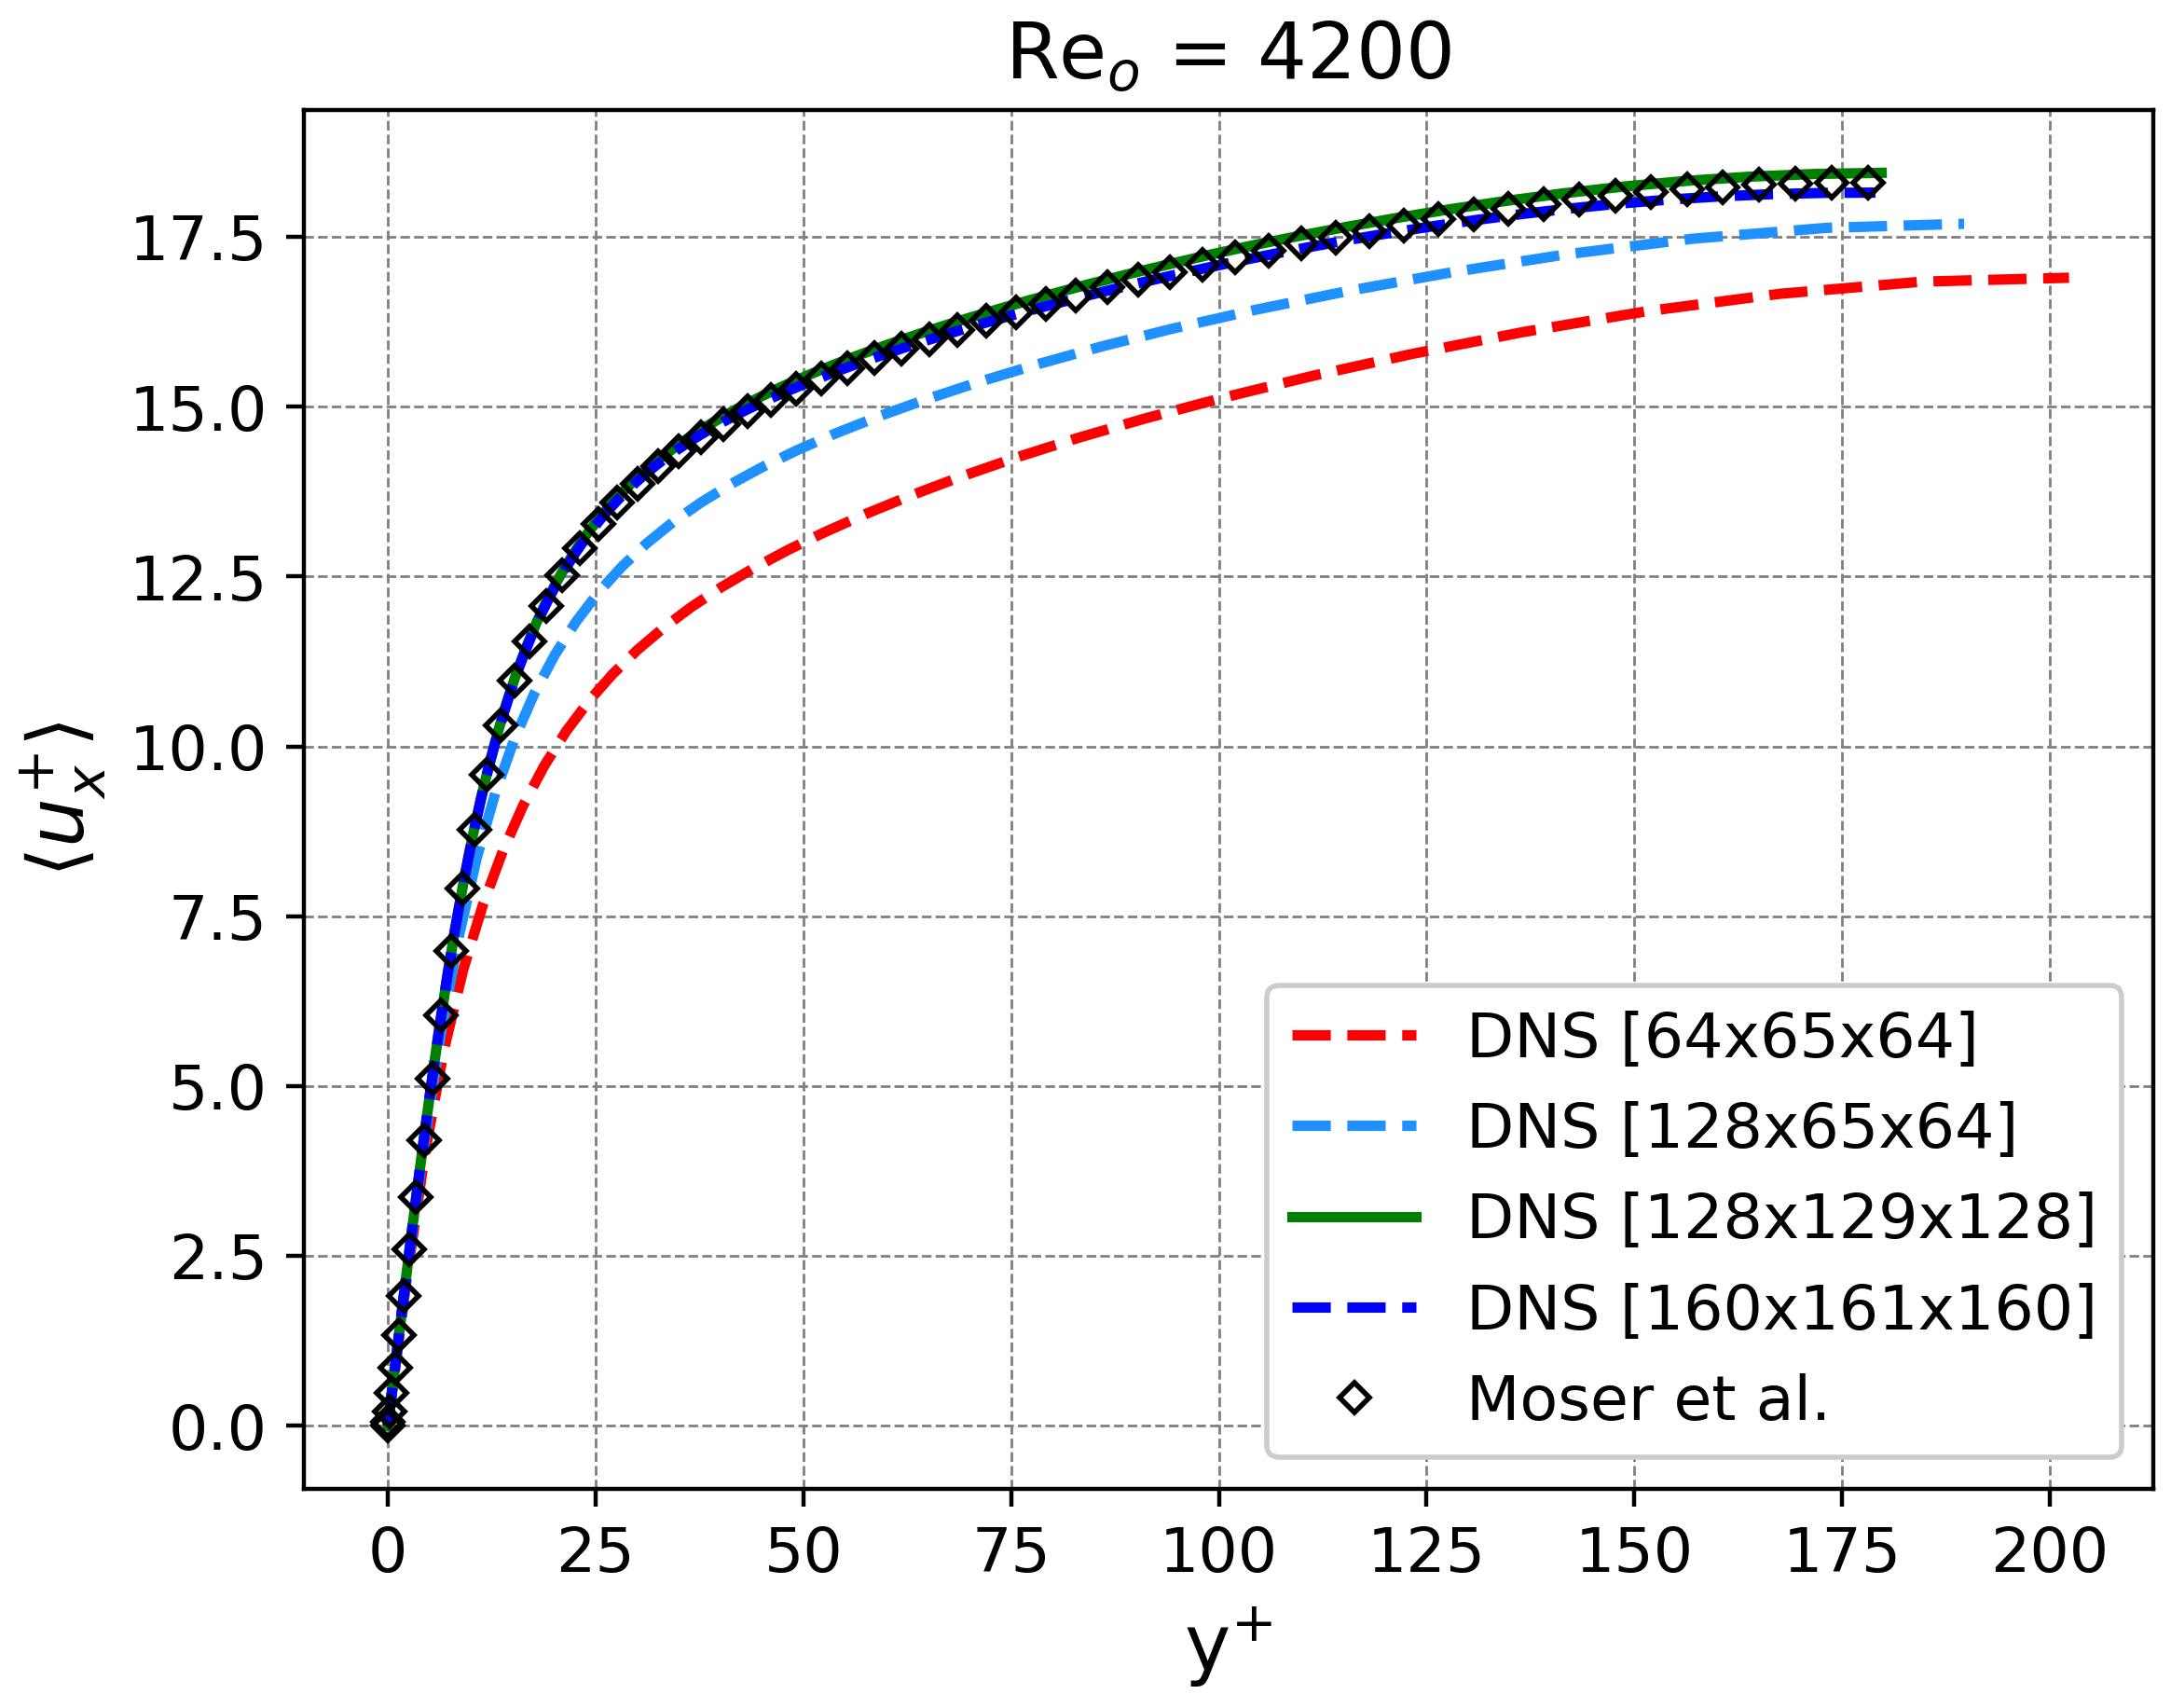
\includegraphics[width=0.49\textwidth]{figures/cap4/kim/ux_mean.png}
    	\label{fig:kim-ux}}  
    \subfloat[]{
    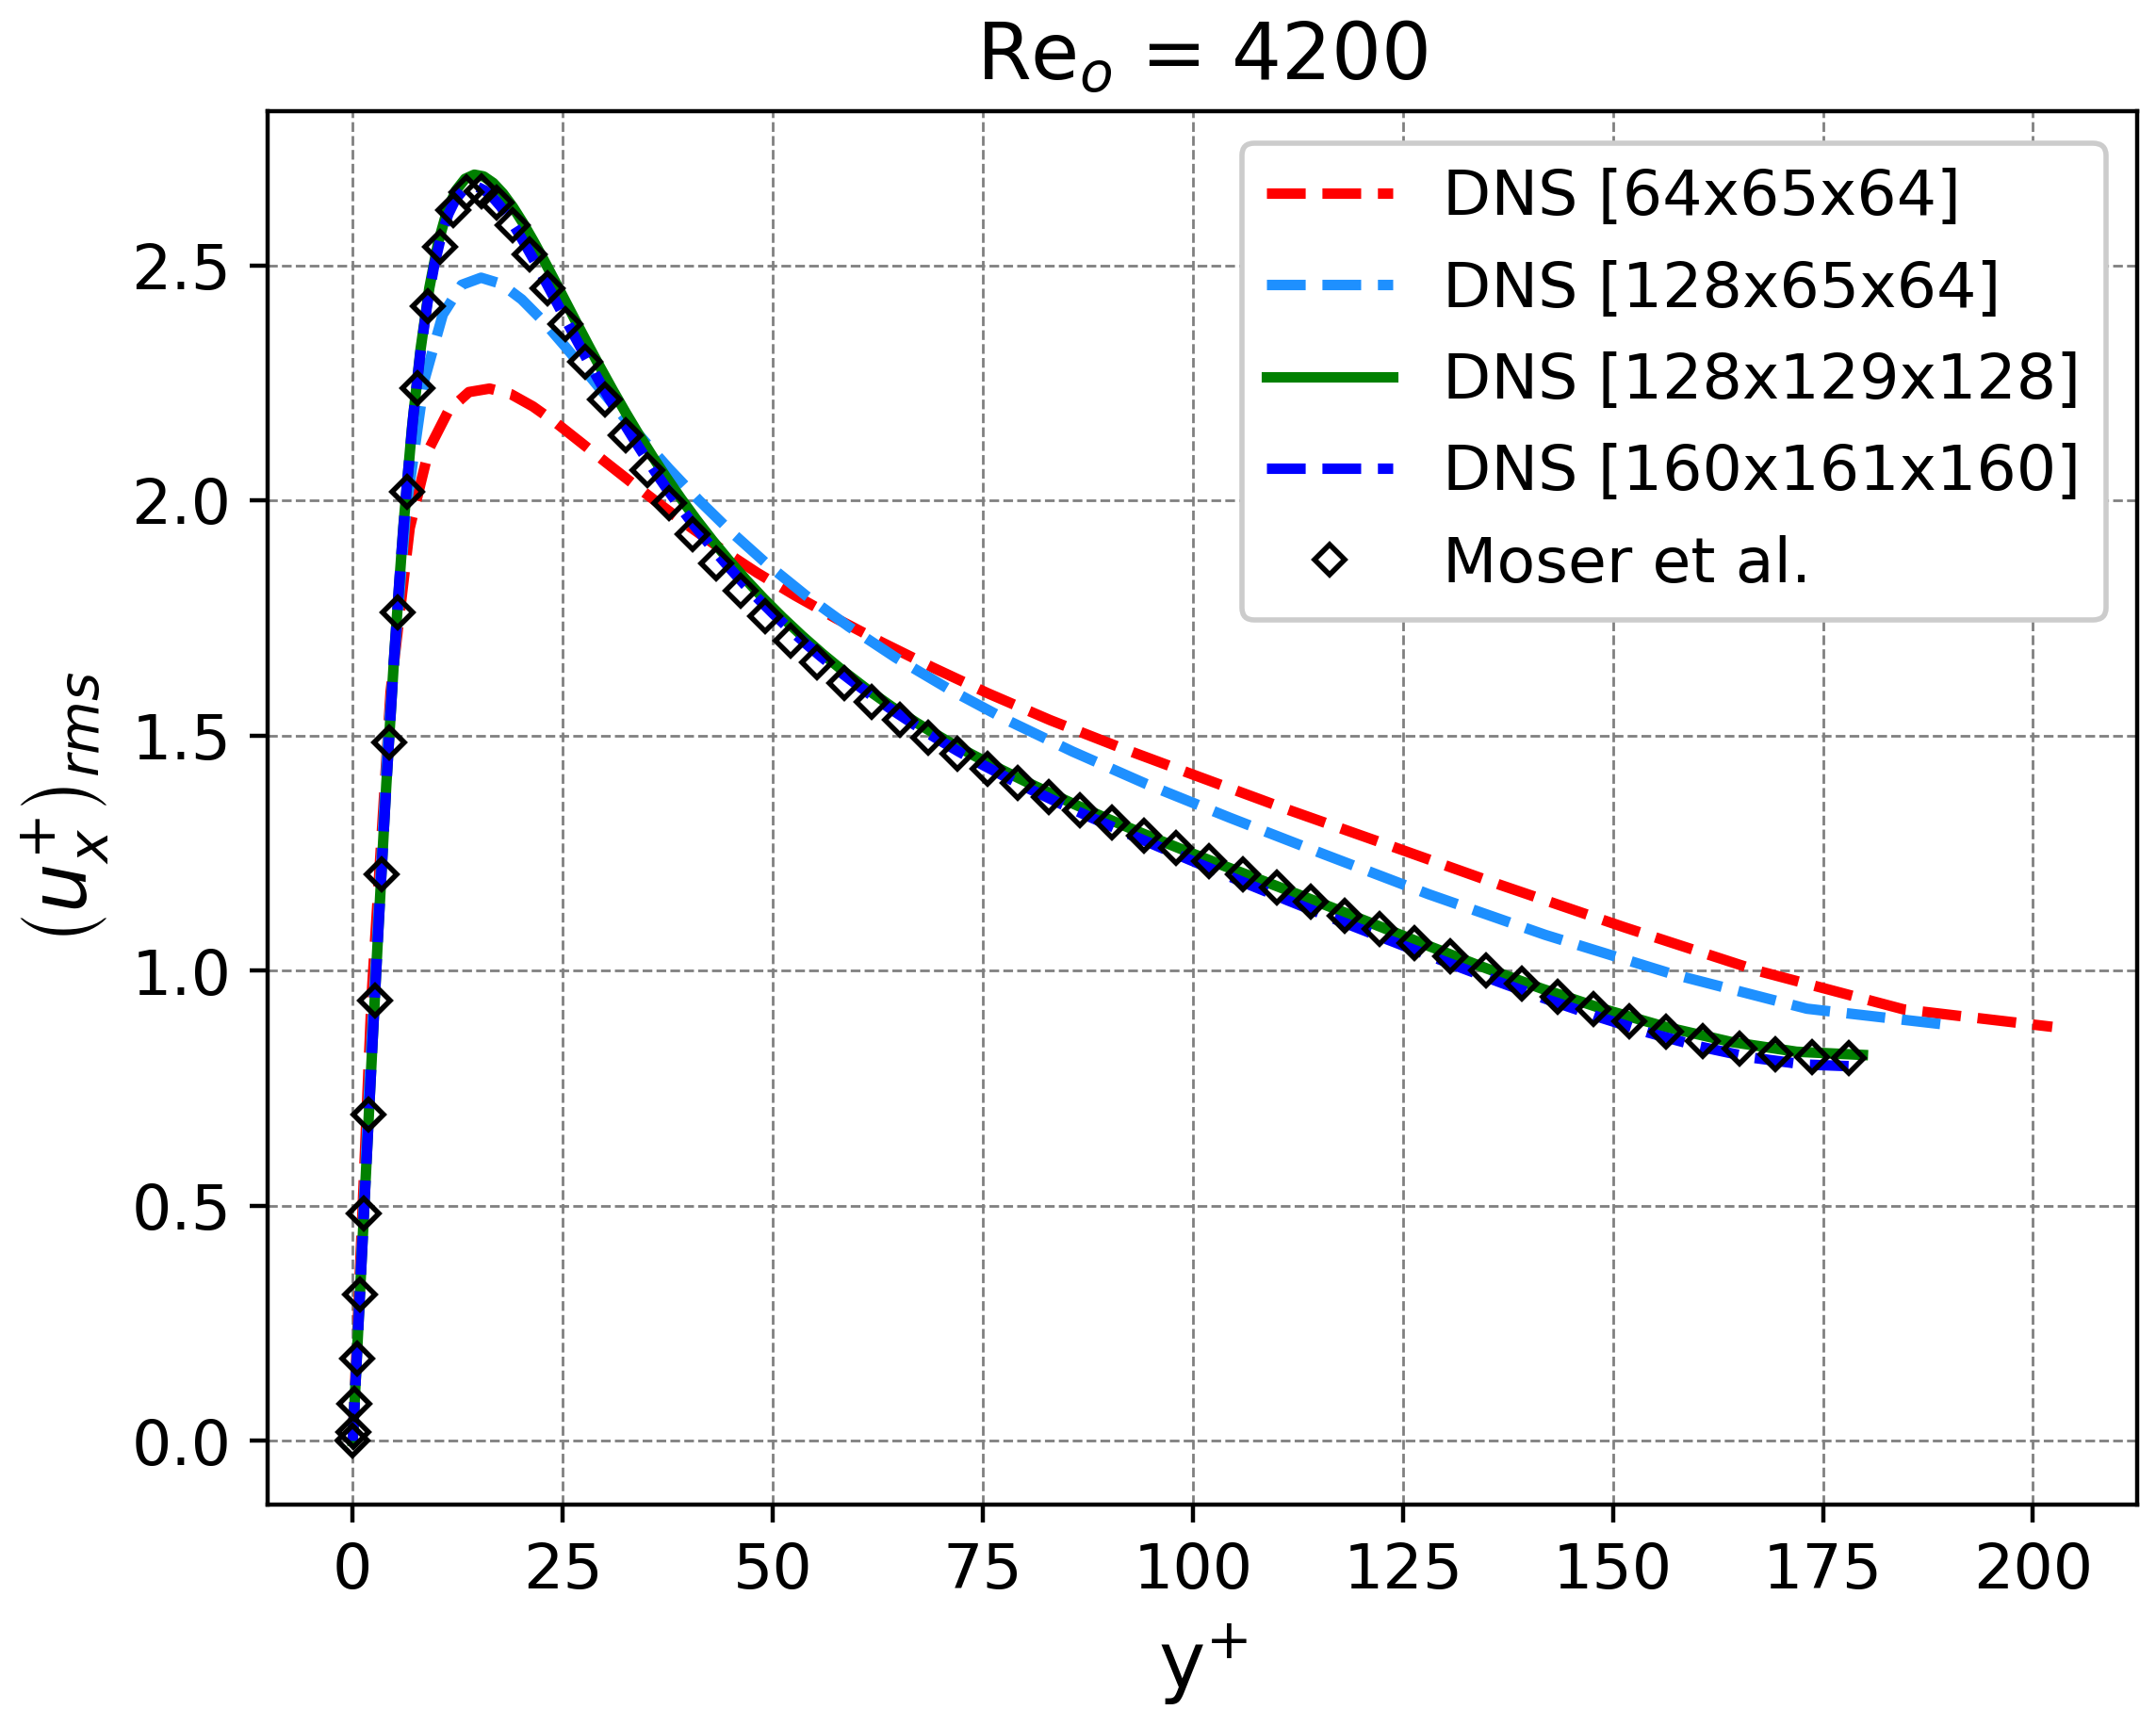
\includegraphics[width=0.49\textwidth]{figures/cap4/kim/ux_rms.png}
    	\label{fig:kim-ux-rms}}
    
    \subfloat[]{
    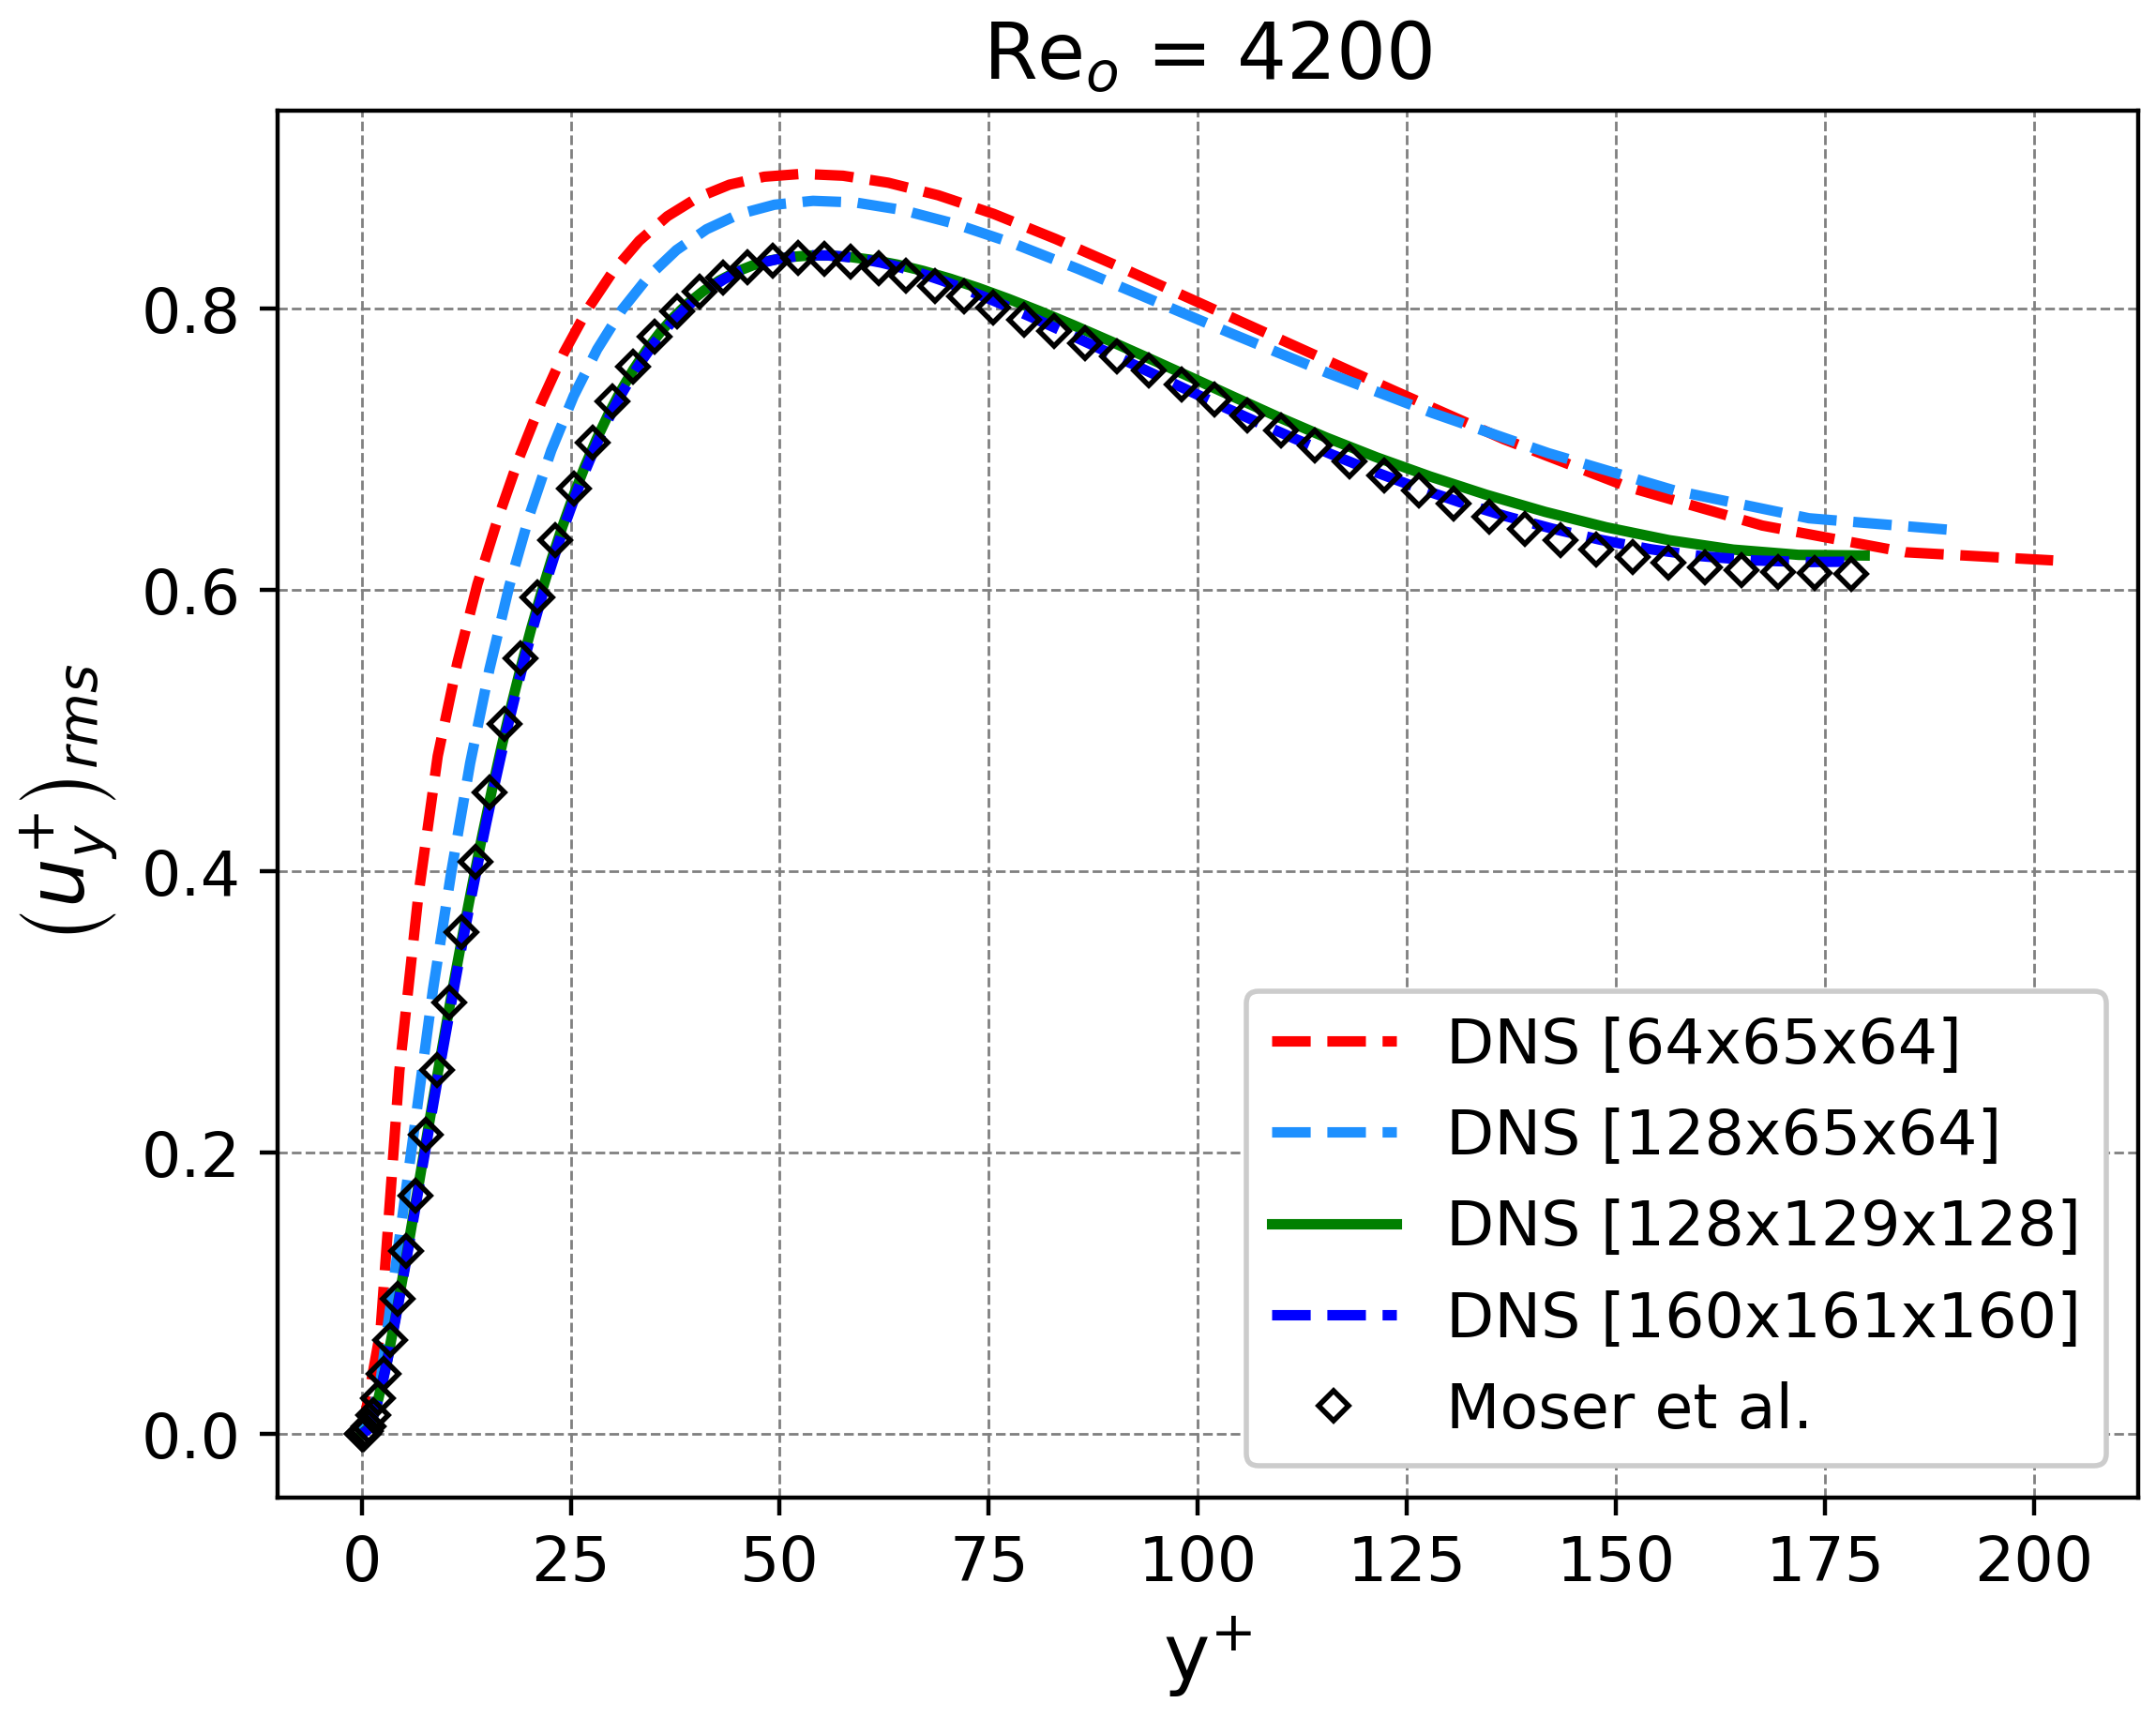
\includegraphics[width=0.49\textwidth]{figures/cap4/kim/uy_rms.png}
    	\label{fig:kim-uy}}  
    \subfloat[]{
    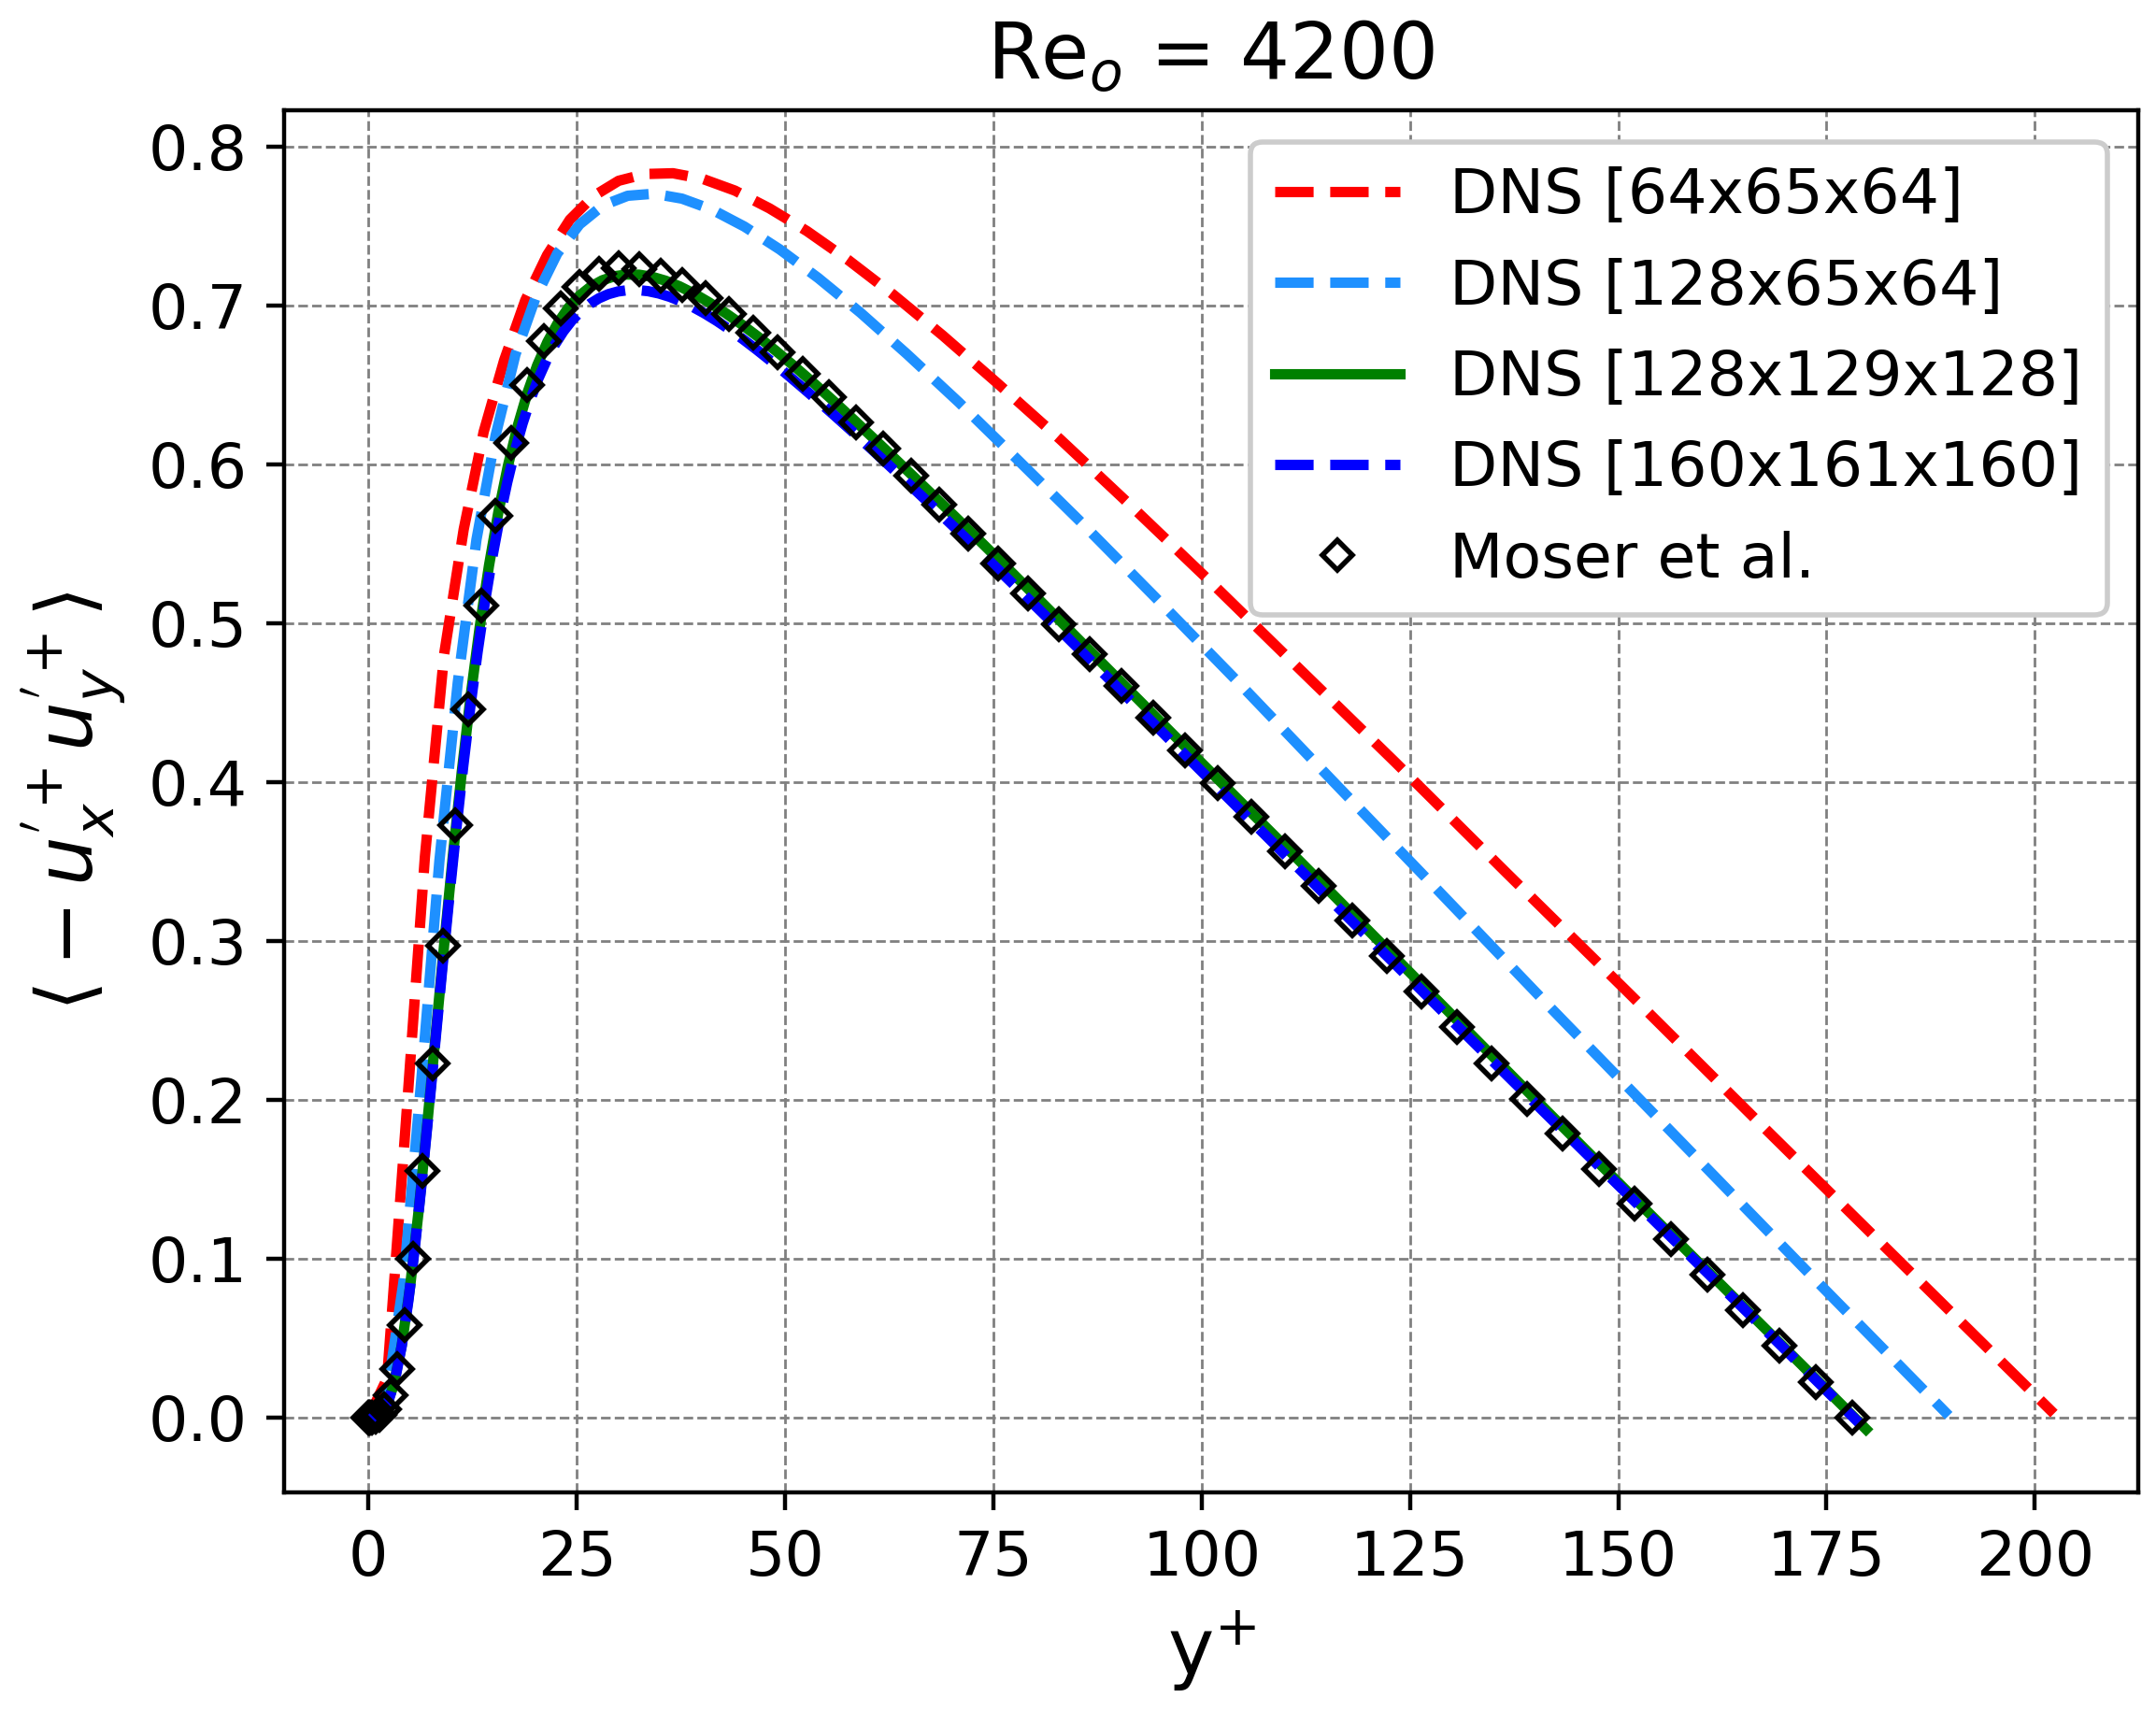
\includegraphics[width=0.49\textwidth]{figures/cap4/kim/up_vp.png}
    	\label{fig:kim-uxuy}} 
 \caption{Perfiles de \textbf{(a)} velocidad media \textit{streamwise}, \textbf{(b)} fluctuaciones RMS de la velocidad en $\langle u^+_x \rangle$, \textbf{(c)} fluctuaciones RMS de la velocidad $\langle u^+_y \rangle$ y \textbf{(d)} componente \textit{XY} del tensor de Reynolds. } 
 \label{fig:kim_1}
\end{figure}

En las Figuras \ref{fig:kim-ux} - \ref{fig:kim-uxuy} se presentan (respectivamente) algunas magnitudes de interés para este sistema: el perfil de velocidad \textit{streamwise} $\langle u^+_x \rangle$ y los perfiles de las componentes del tensor de Reynolds\footnote{La raíz cuadrada de una componente diagonal en una dirección \textit{i} arbitraria del tensor de Reynolds, es equivalente a la fluctuación de la velocidad en dicha dirección. Esto es, $(u_i)_{rms} = \sqrt{ \langle u^{\prime}_i u^{\prime}_i} \rangle $.} $\sqrt{\langle u^{+ \prime}_x u^{+ \prime}_x \rangle}$, $\sqrt{\langle u^{+ \prime}_y u^{+ \prime}_y \rangle}$ y $\langle u^{+ \prime}_x u^{+ \prime}_y \rangle$. En estas graficas se comparan las distintas mallas empleadas con el trabajo de Moser \textit{et al.} \cite{moser1999}. Por un lado es posible apreciar la convergencia en malla, y por el otro, se observa que los datos obtenidos mediante la simulación DNS con XC3D son completamente consistentes con aquellos datos de referencia.

\subsection{Situación II. Transporte de escalar pasivo en convección forzada con $q''_w$ constante}

En este caso se considera sólo el régimen de convección forzada, lo que equivale a suponer $\Pi=0$ en la ecuación de momento. De esta forma, las ecuaciones de continuidad y momento quedan desacopladas de la ecuación de energía (ecuaciones \ref{eq:gob_system_adim}). En este sentido, los campos solución de la velocidad son exactamente los mismos que en la \textbf{Situación I} y el campo de temperatura es un campo escalar que no interviene en el desarrollo hidrodinámico del sistema, sino únicamente en el aspecto térmico del flujo. Por ello, sólo se presentan magnitudes asociadas a la temperatura adimensional. Para las simulaciones asociadas a esta sub-sección, se considera el número de Reynolds Re$_o=4278$. 

\paragraph{Convergencia en Malla.}
En primer lugar, se analiza la respuesta del campo escalar solución frente a diferentes mallas, en concreto, se emplean aquellas mismas utilizadas en la \textbf{Situación I}.  Las Figuras \ref{fig:kmesh-theta} - \ref{fig:kmesh-uy-theta} presentan los perfiles de la temperatura adimensional, sus fluctuaciones y los flujos de calor turbulento en las direcciones X e Y, respectivamente. Las simulaciones propias se comparan con aquellas obtenidas en la referencia \textit{et al.} \cite{kawamura2000dns} para Pr=0.71. Además, en dichas gráficas se exponen los distintos resultados obtenidos por Kawamura \textit{et al.} para diferentes mallas empleadas en su trabajo. 

De la misma forma que ocurre en el caso anterior, es posible observar claramente la convergencia en malla, y como, a medida que aumenta la precisión en las simulaciones, los resultados obtenidos presentan un buen acuerdo con los aquellos de referencia. En particular, es posible observar que la malla M2 resulta suficiente para replicar los resultados de los trabajos \cite{moser1999, kawamura2000dns}.

\begin{figure}[H]
 \centering
    \subfloat[]{
    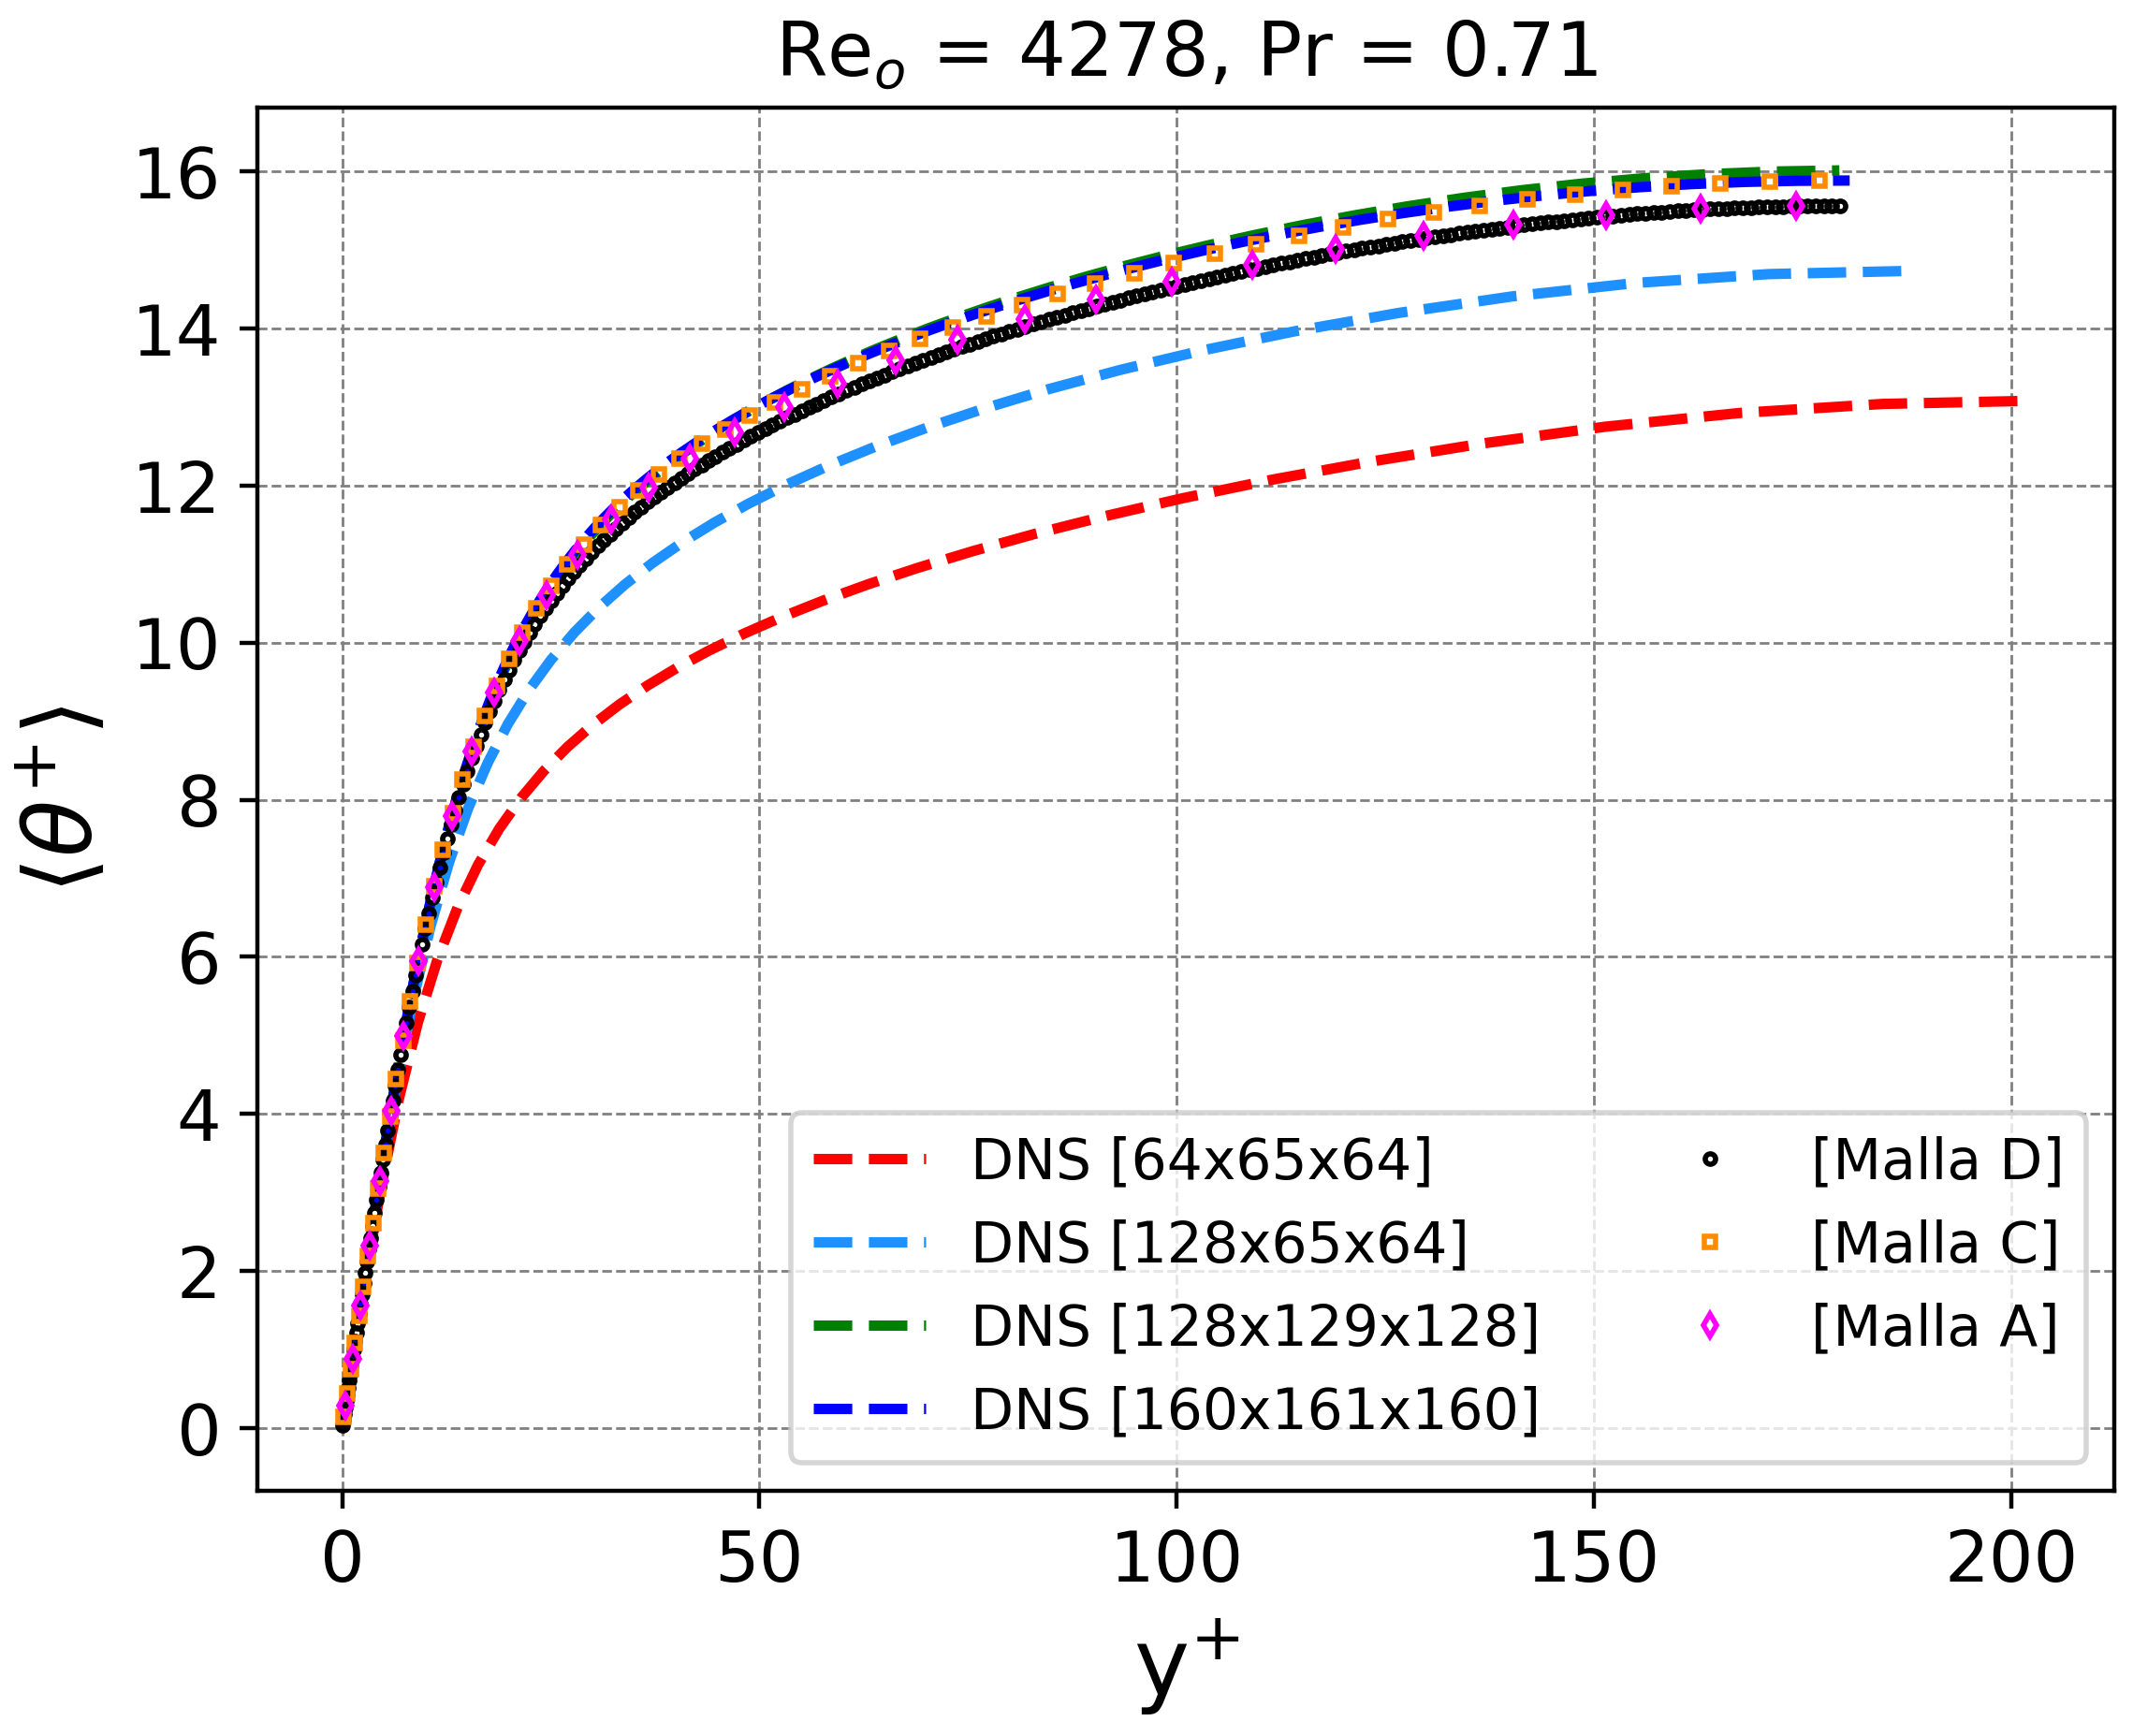
\includegraphics[width=0.49\textwidth]{figures/cap4/kawamura_mesh/tep_theta.png}
    	\label{fig:kmesh-theta}}  
    \subfloat[]{
    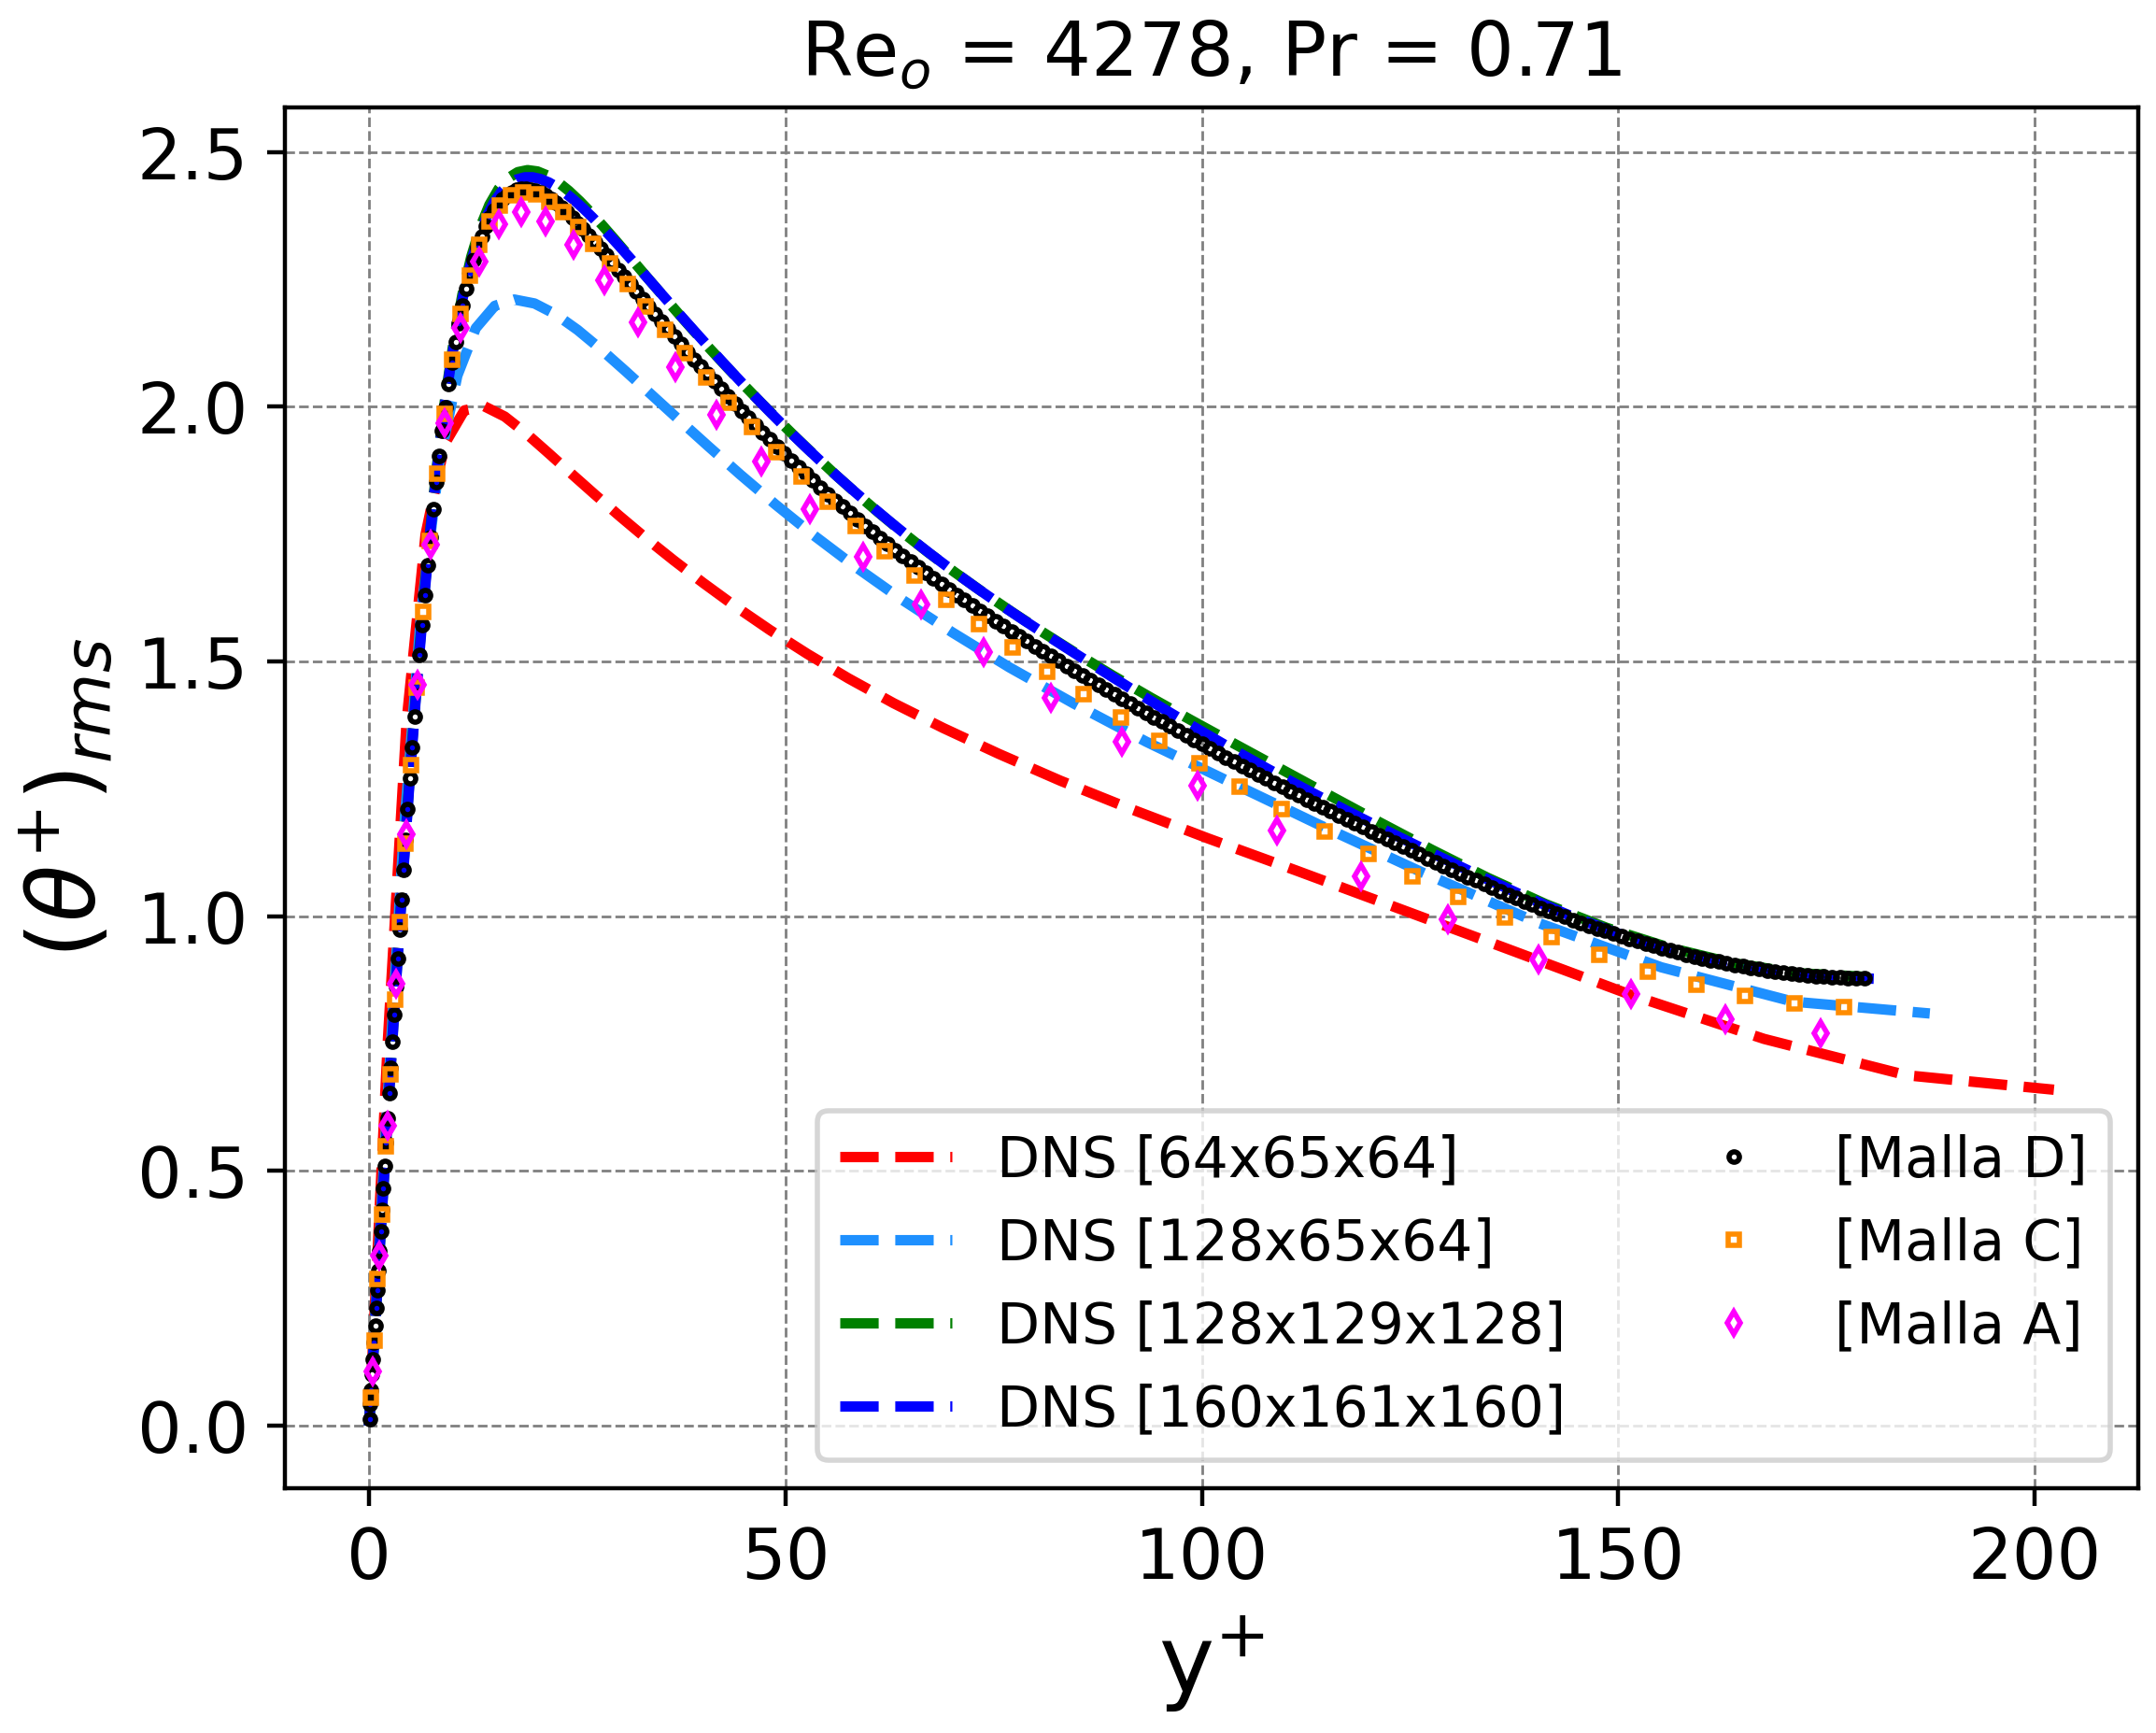
\includegraphics[width=0.49\textwidth]{figures/cap4/kawamura_mesh/tep_thetap_rms.png}
    	\label{fig:kmesh-theta-rms}}  

    \subfloat[]{
    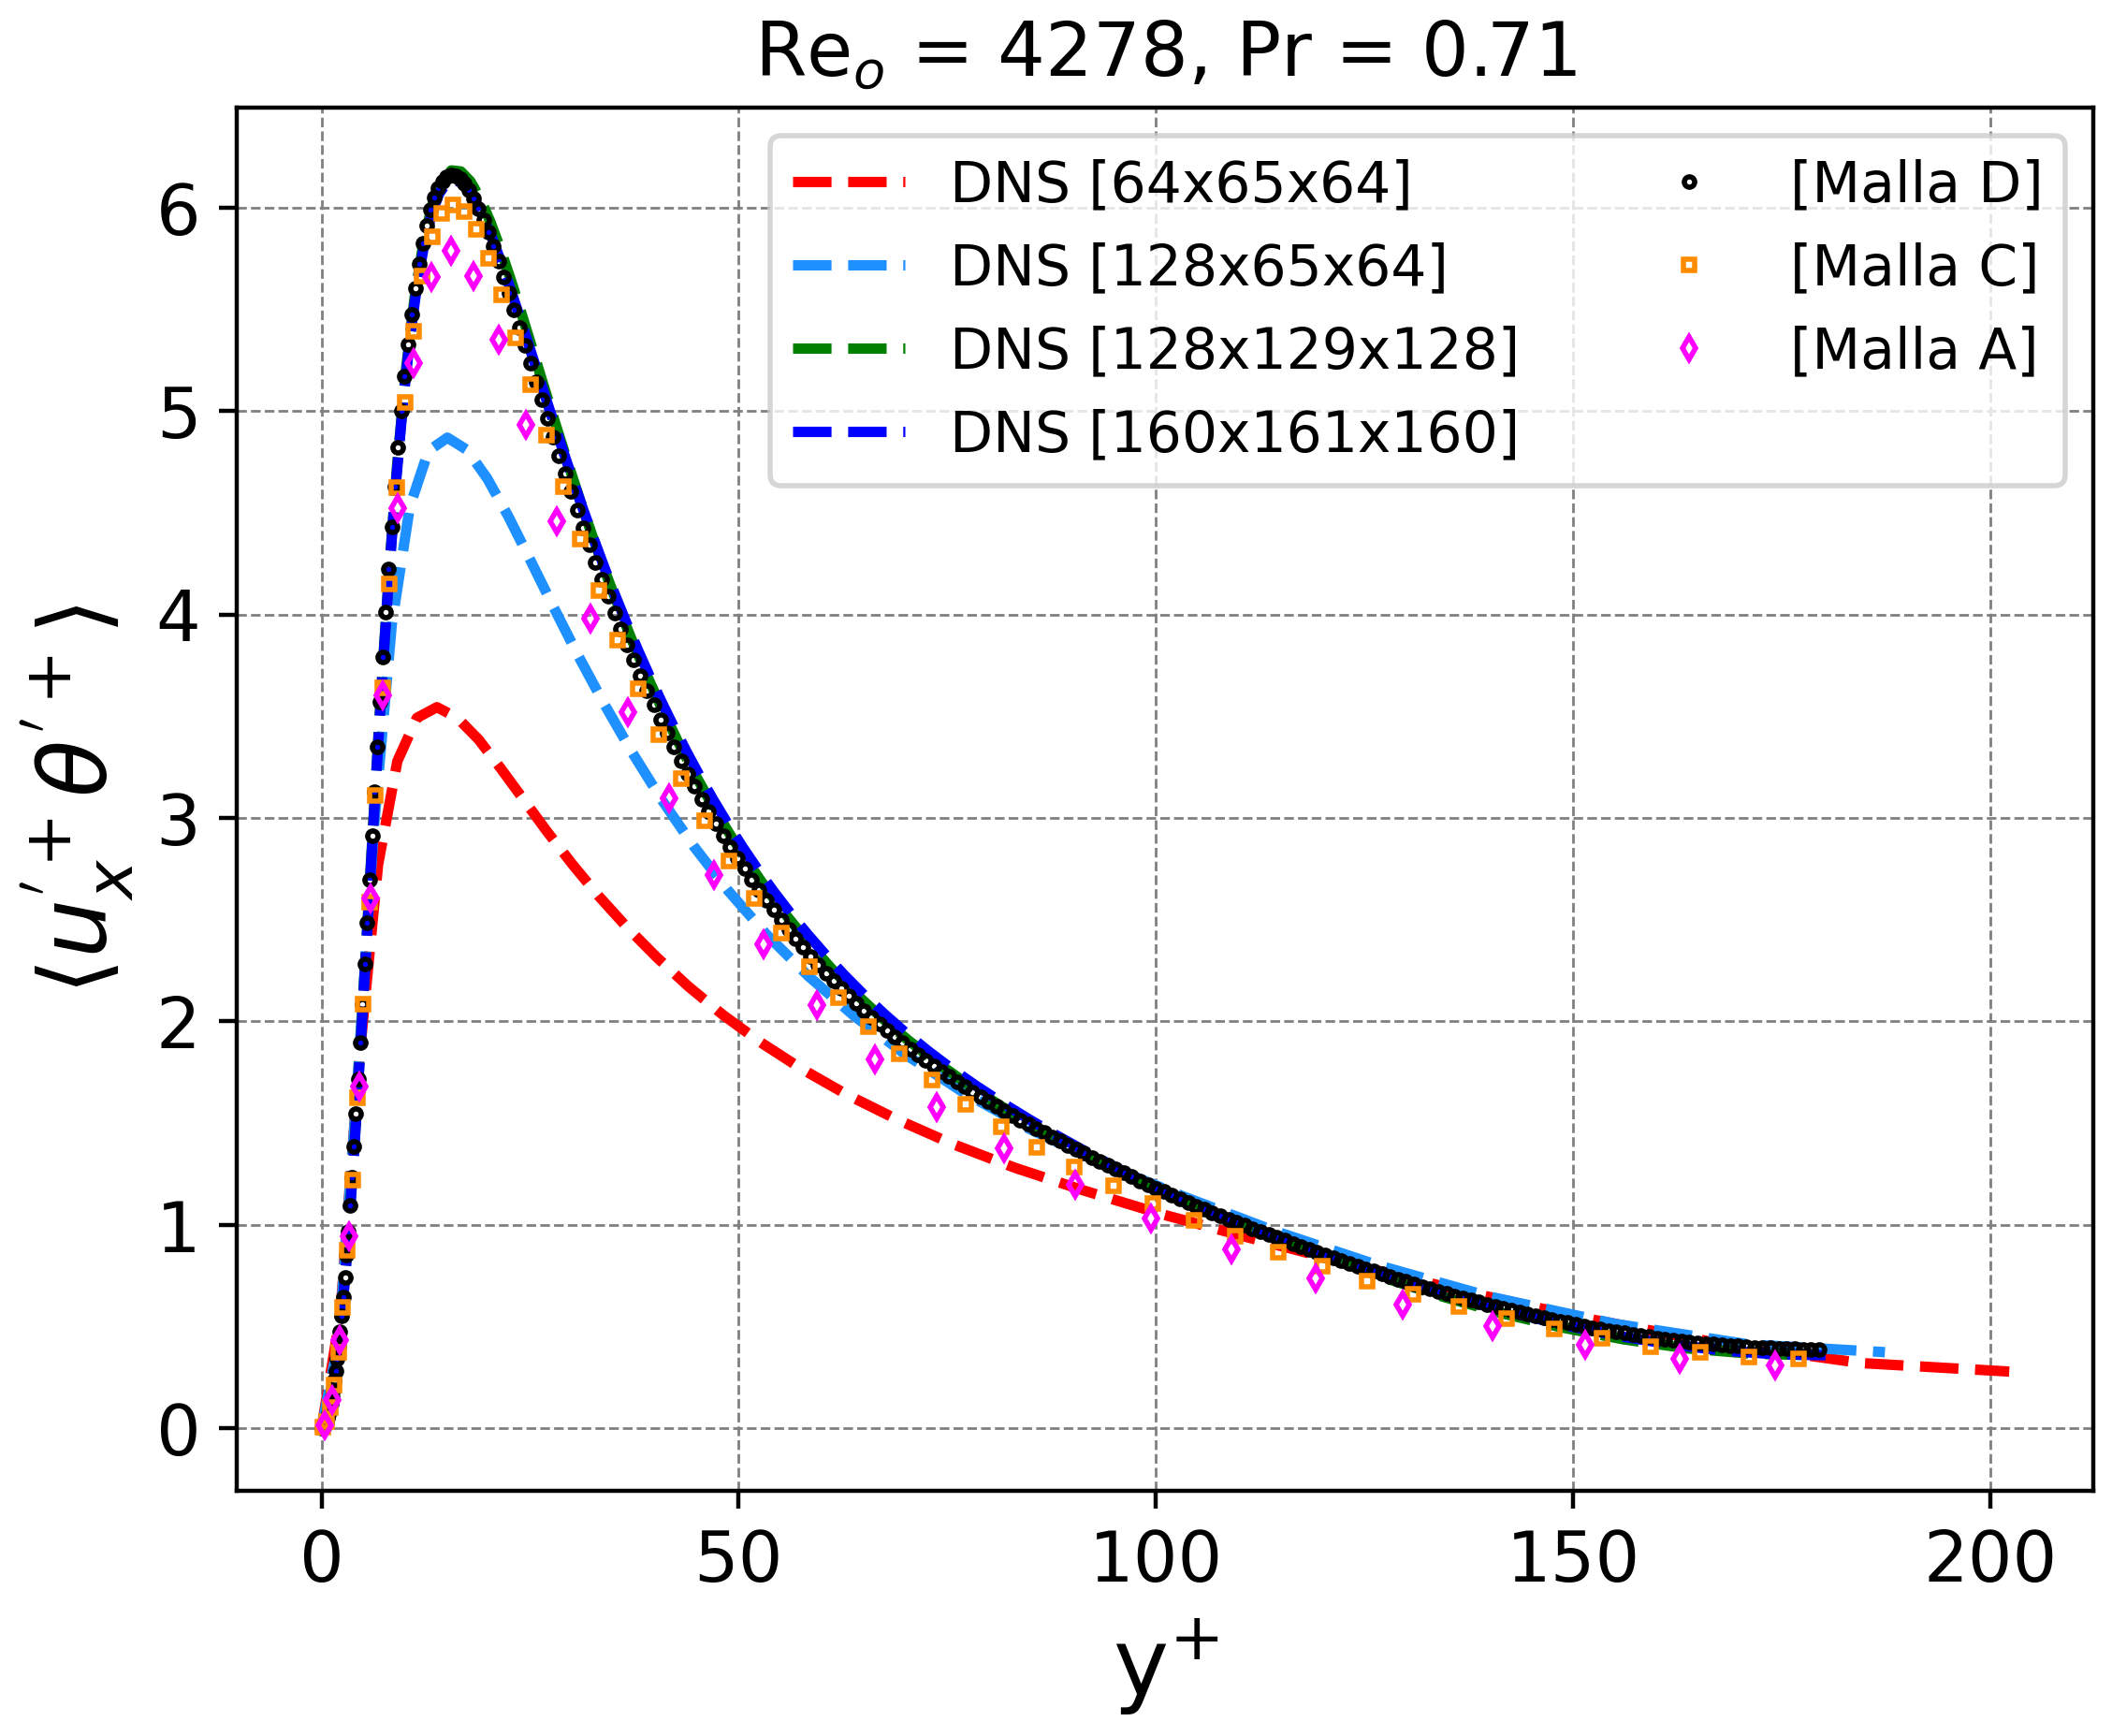
\includegraphics[width=0.49\textwidth]{figures/cap4/kawamura_mesh/tep_up_thetap.png}
    	\label{fig:kmesh-ux-theta}}  
    \subfloat[]{
    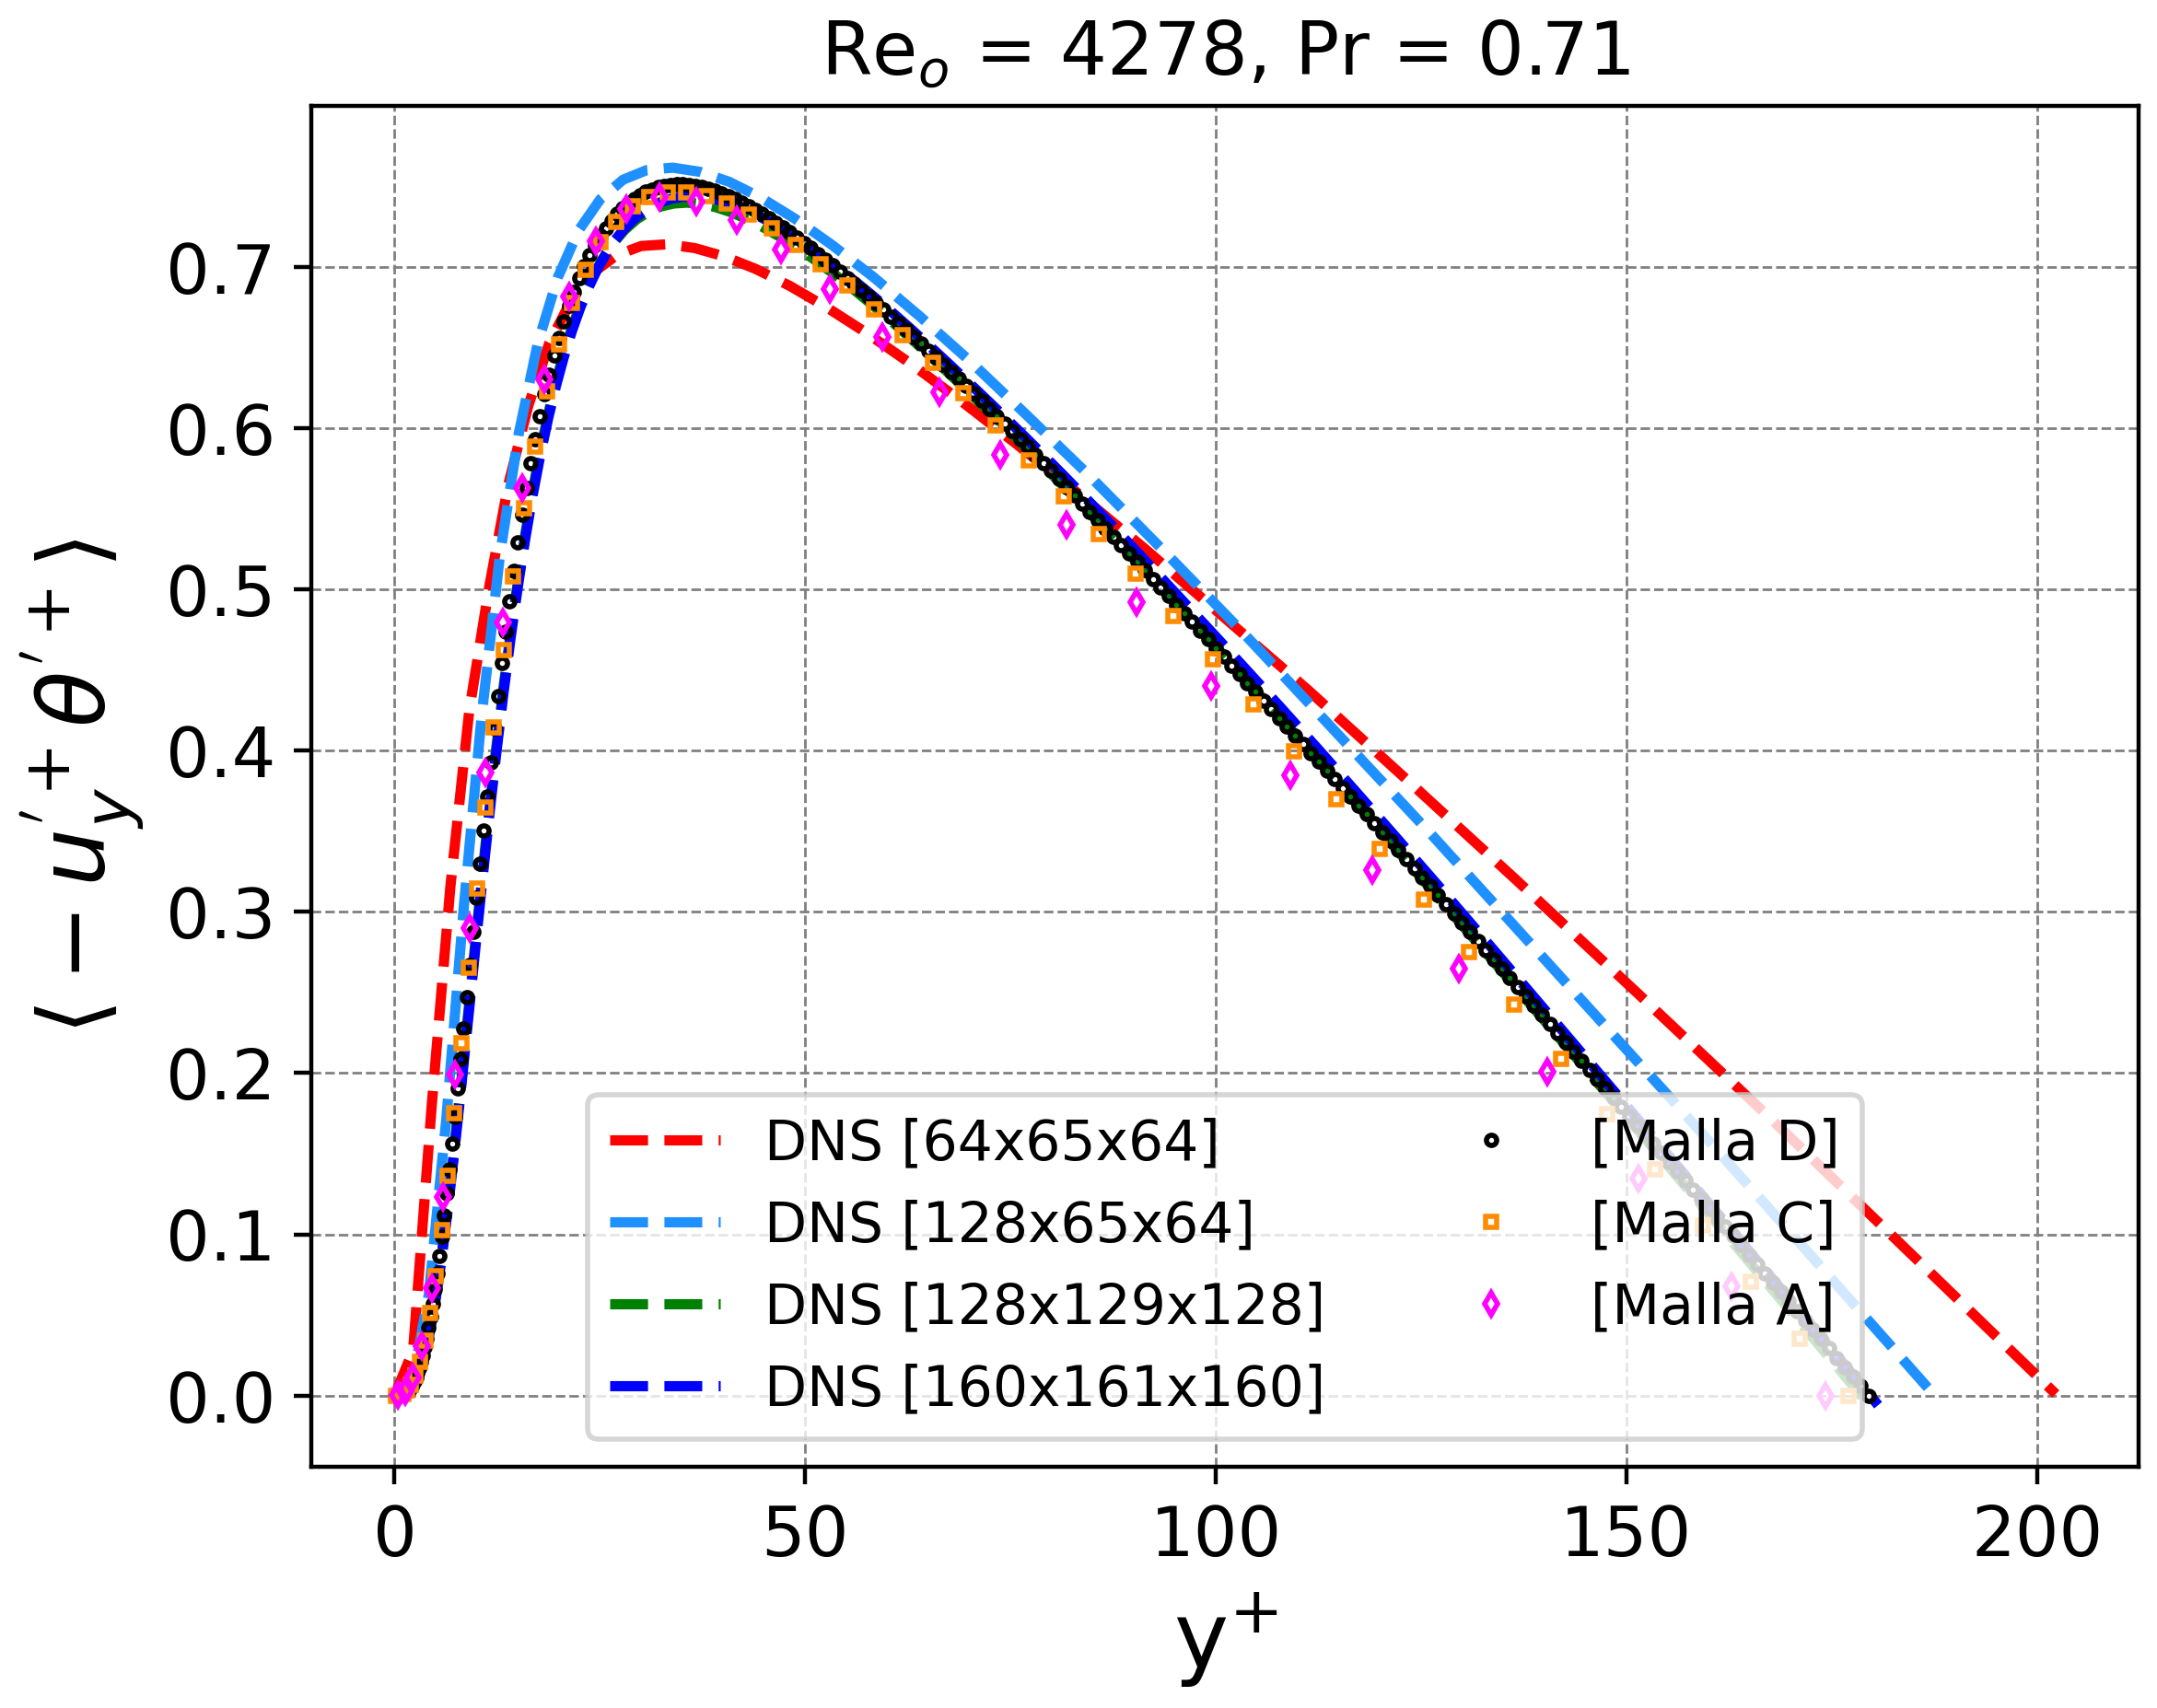
\includegraphics[width=0.49\textwidth]{figures/cap4/kawamura_mesh/tep_vp_thetap.png}
    	\label{fig:kmesh-uy-theta}}  
 \caption{Perfiles de \textbf{(a)} temperatura adimensional media, \textbf{(b)} fluctuaciones RMS de la temperatura adimensional, \textbf{(c)} flujo de calor turbulento en la dirección X, $\langle u^+_x \theta^+ \rangle$, y \textbf{(d)} flujo de calor turbulento en la dirección Y, $\langle u^+_y \theta^+ \rangle$.} 
 \label{fig:kmesh_1}
\end{figure}

\paragraph{Variación del número de Prandtl.}
La segunda parte consiste en emplear la malla M2 para distintos números de Prandtl, en particular, aquellos empleados en el trabajo de Kawamura \textit{et al.}: Pr= 0.025, 0.71, 1 y 7. De igual forma que para la convergencia en malla, en las Figuras \ref{fig:kpr-theta} - \ref{fig:kpr-uy-theta} se muestran los perfiles de las magnitudes $\langle \theta^+ \rangle$, $(\theta^+)_{rms}$, $\langle u^{+ \prime}_x \theta^{+ \prime} \rangle$ y $\langle - u^{+ \prime}_y \theta^{+ \prime} \rangle$, respectivamente. Se observa que la malla M2 resulta suficiente para replicar con bastante fidelidad las simulaciones de Kawamura \textit{et al.}; sin embargo, a medida que se aumenta el número de Pr, es requerido emplear un rango de evolución temporal mayor para alcanzar el estado estadísticamente estacionario antes de poder colectar estadística.

\begin{figure}[H]
 \centering
  \subfloat[]{
    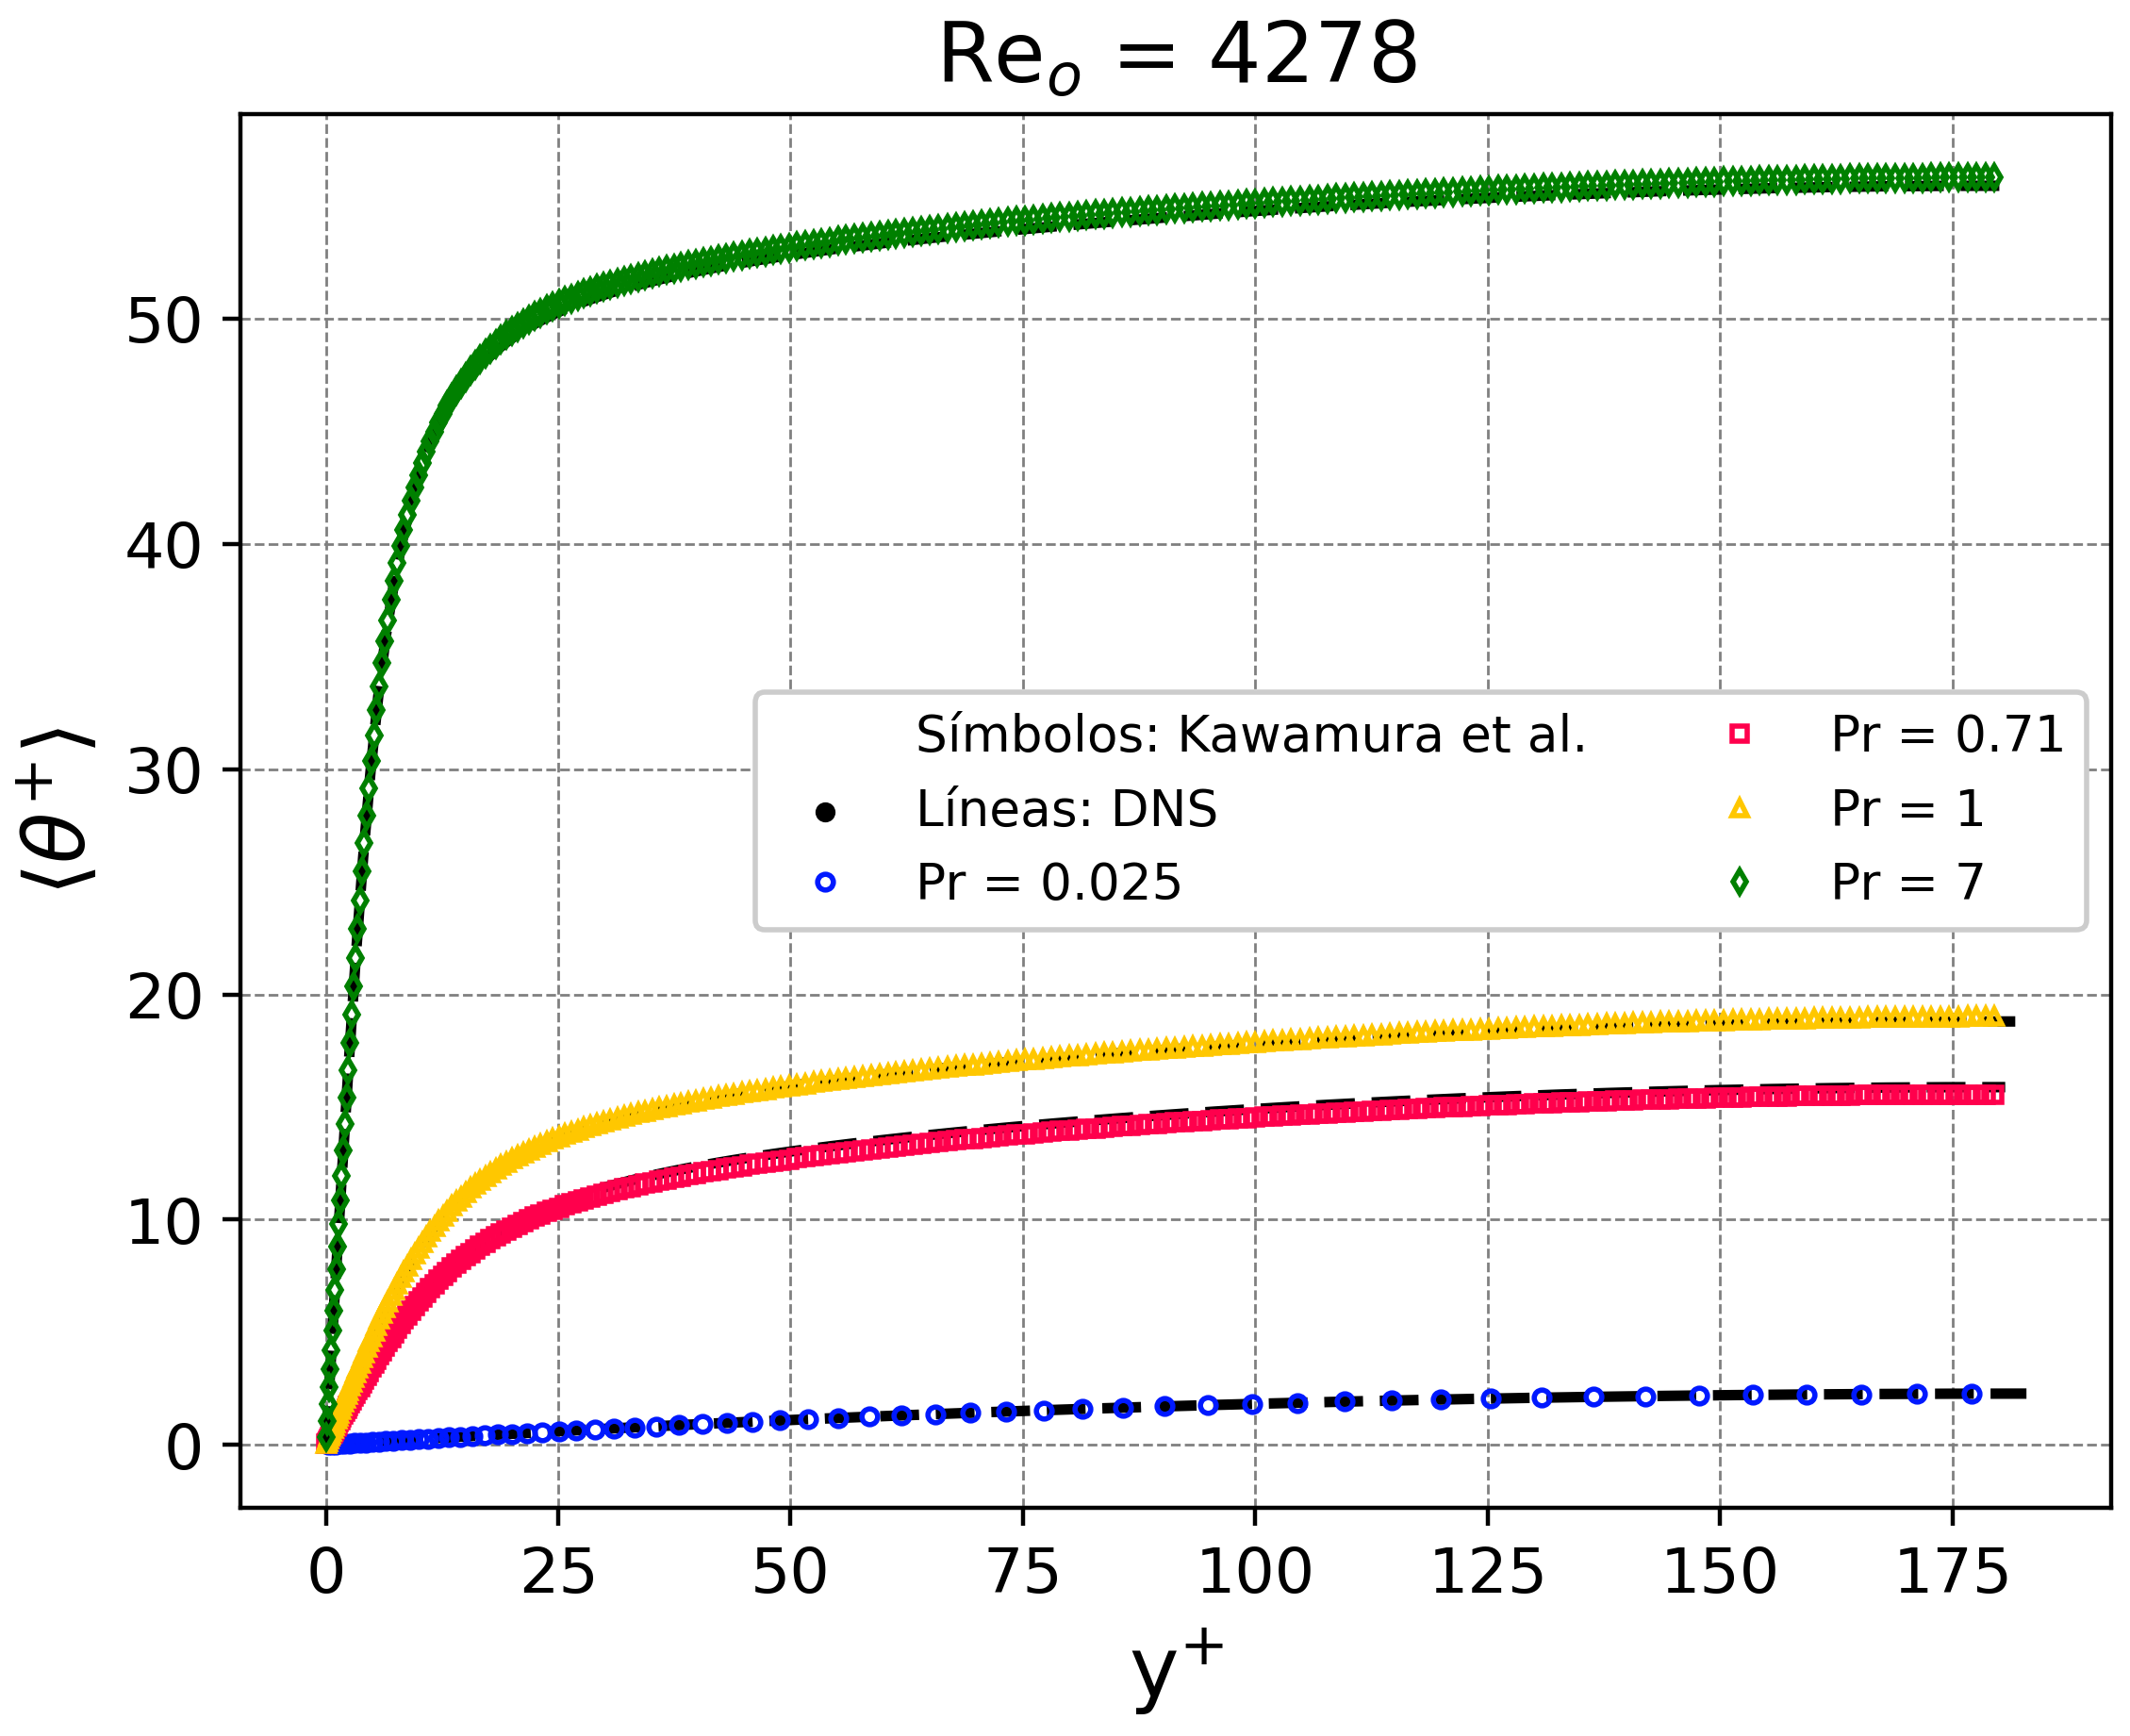
\includegraphics[width=0.49\textwidth]{figures/cap4/kawamura_prs/tep_theta.png}
    \label{fig:kpr-theta}}  
    \subfloat[]{
    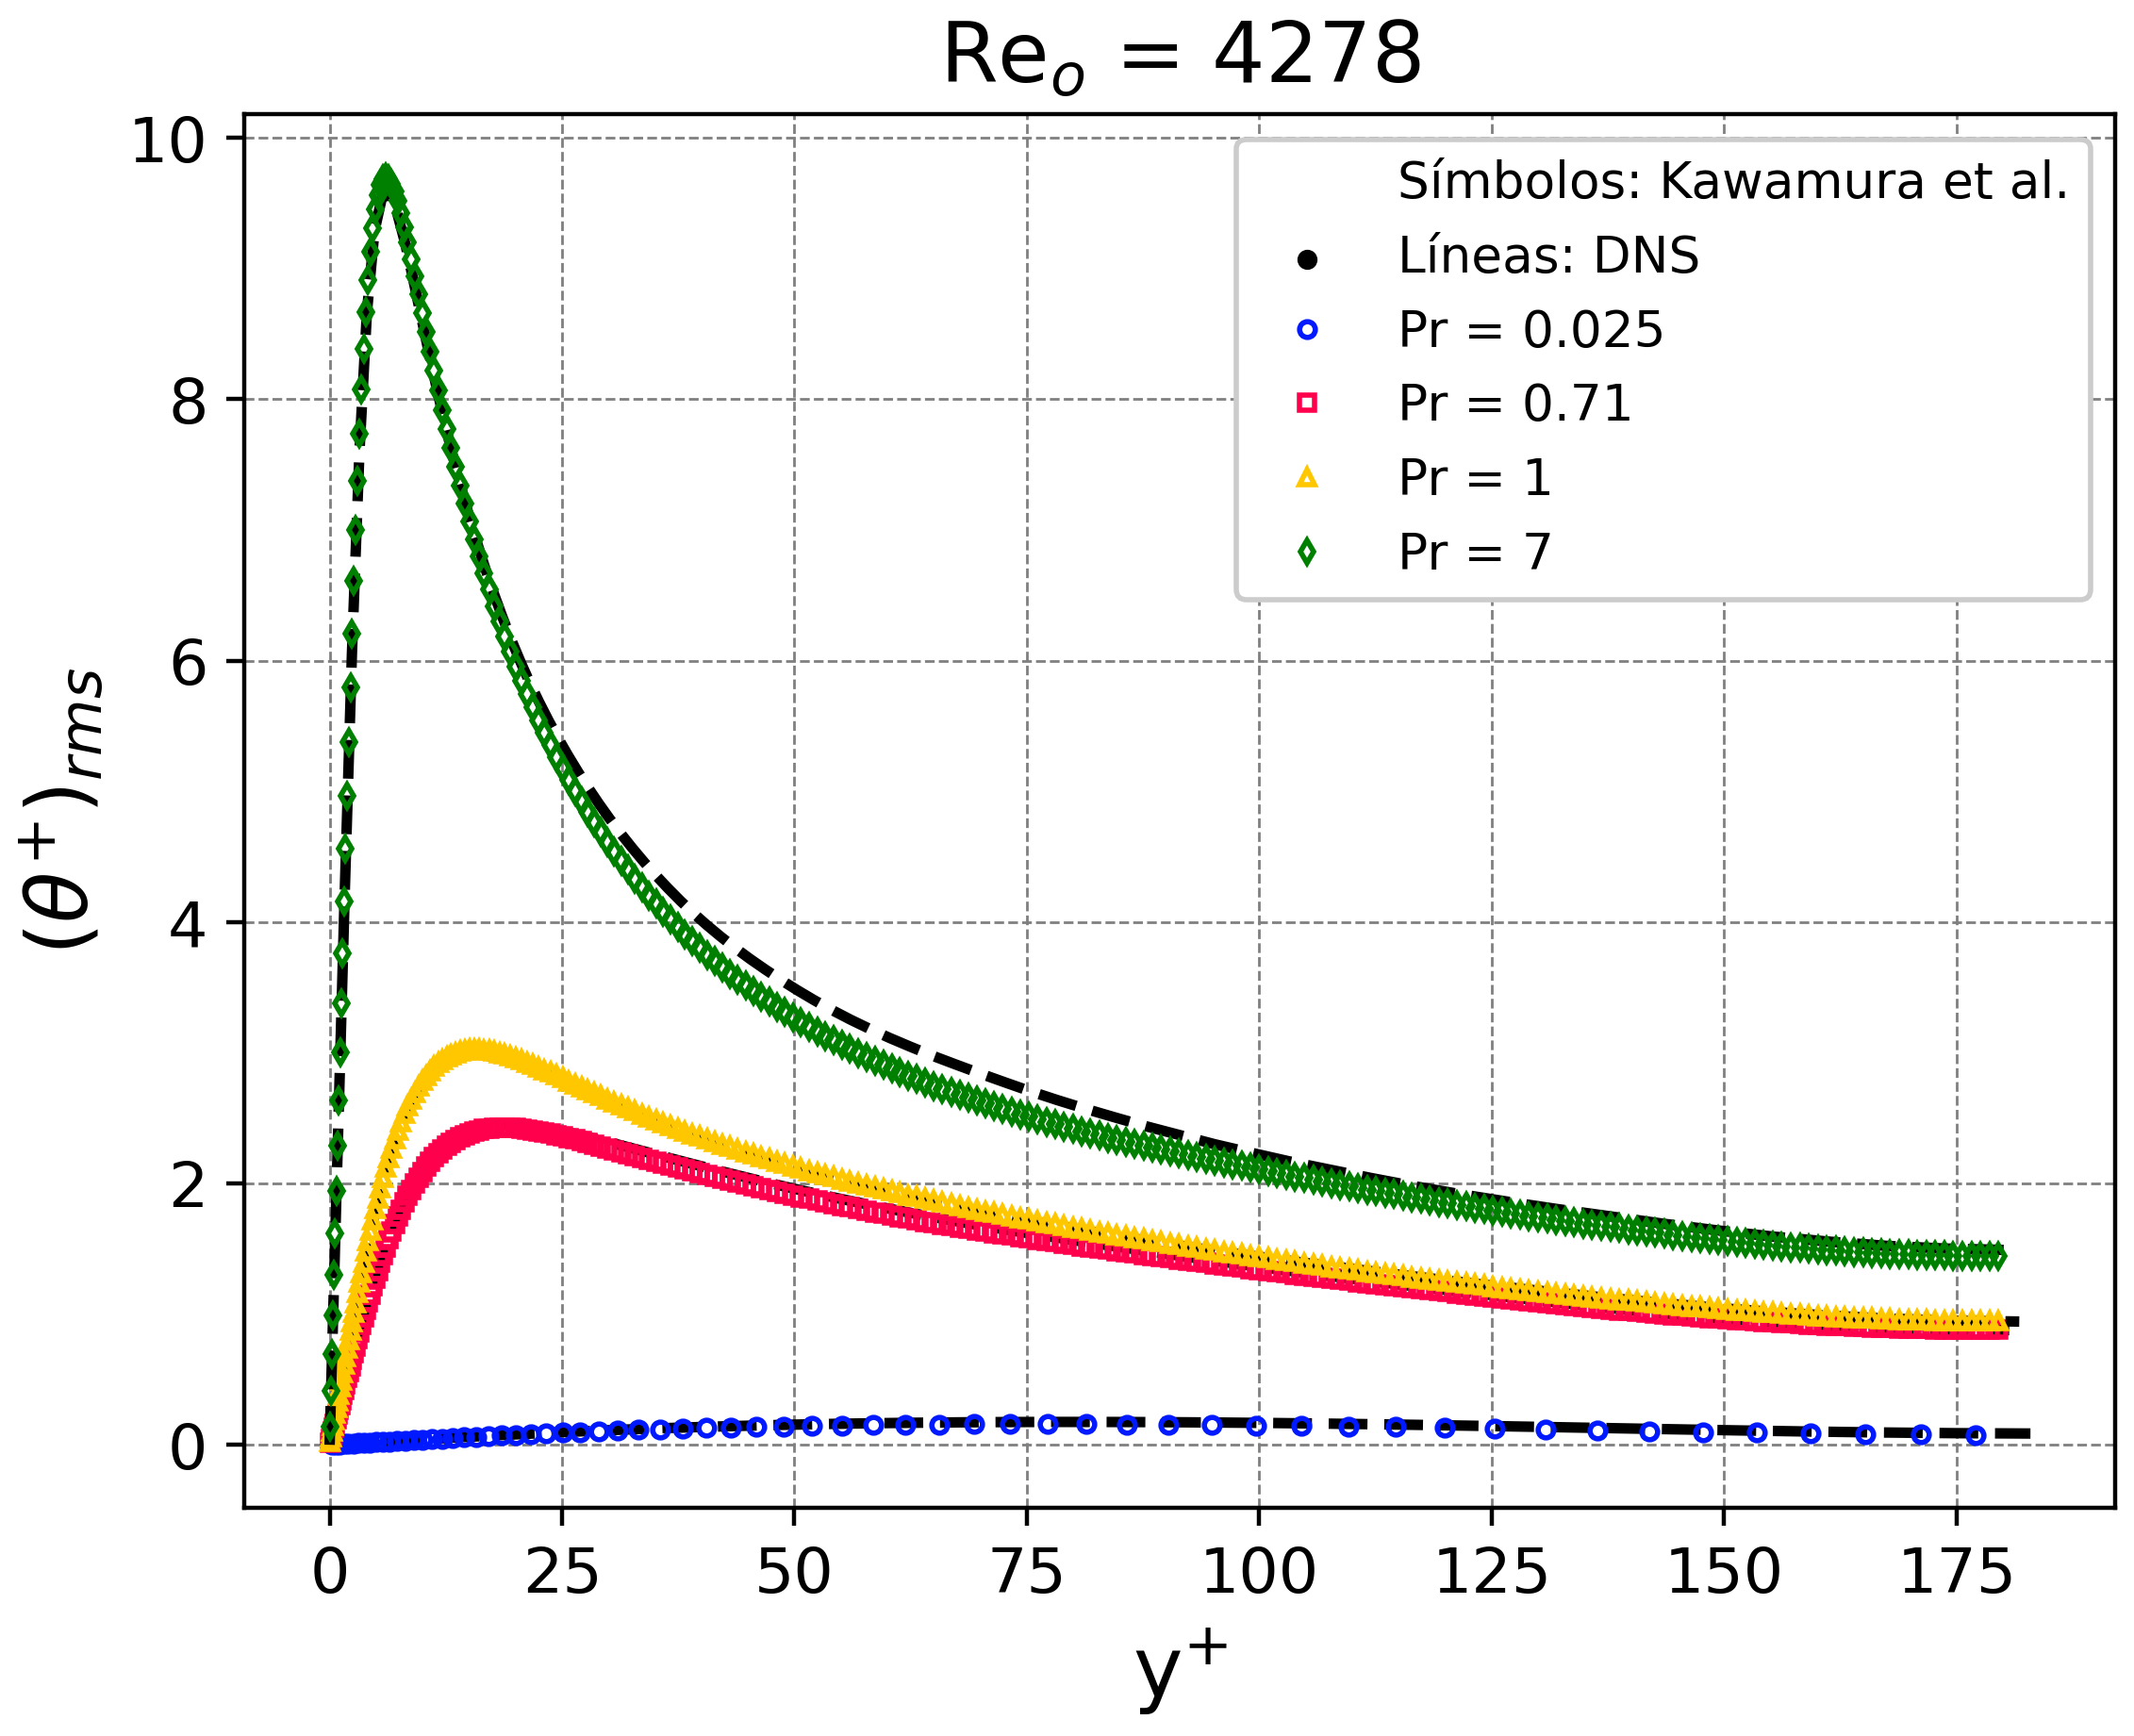
\includegraphics[width=0.49\textwidth]{figures/cap4/kawamura_prs/tep_thetap_rms.png}
    \label{fig:kpr-theta-rms}}  
 
  \subfloat[]{
    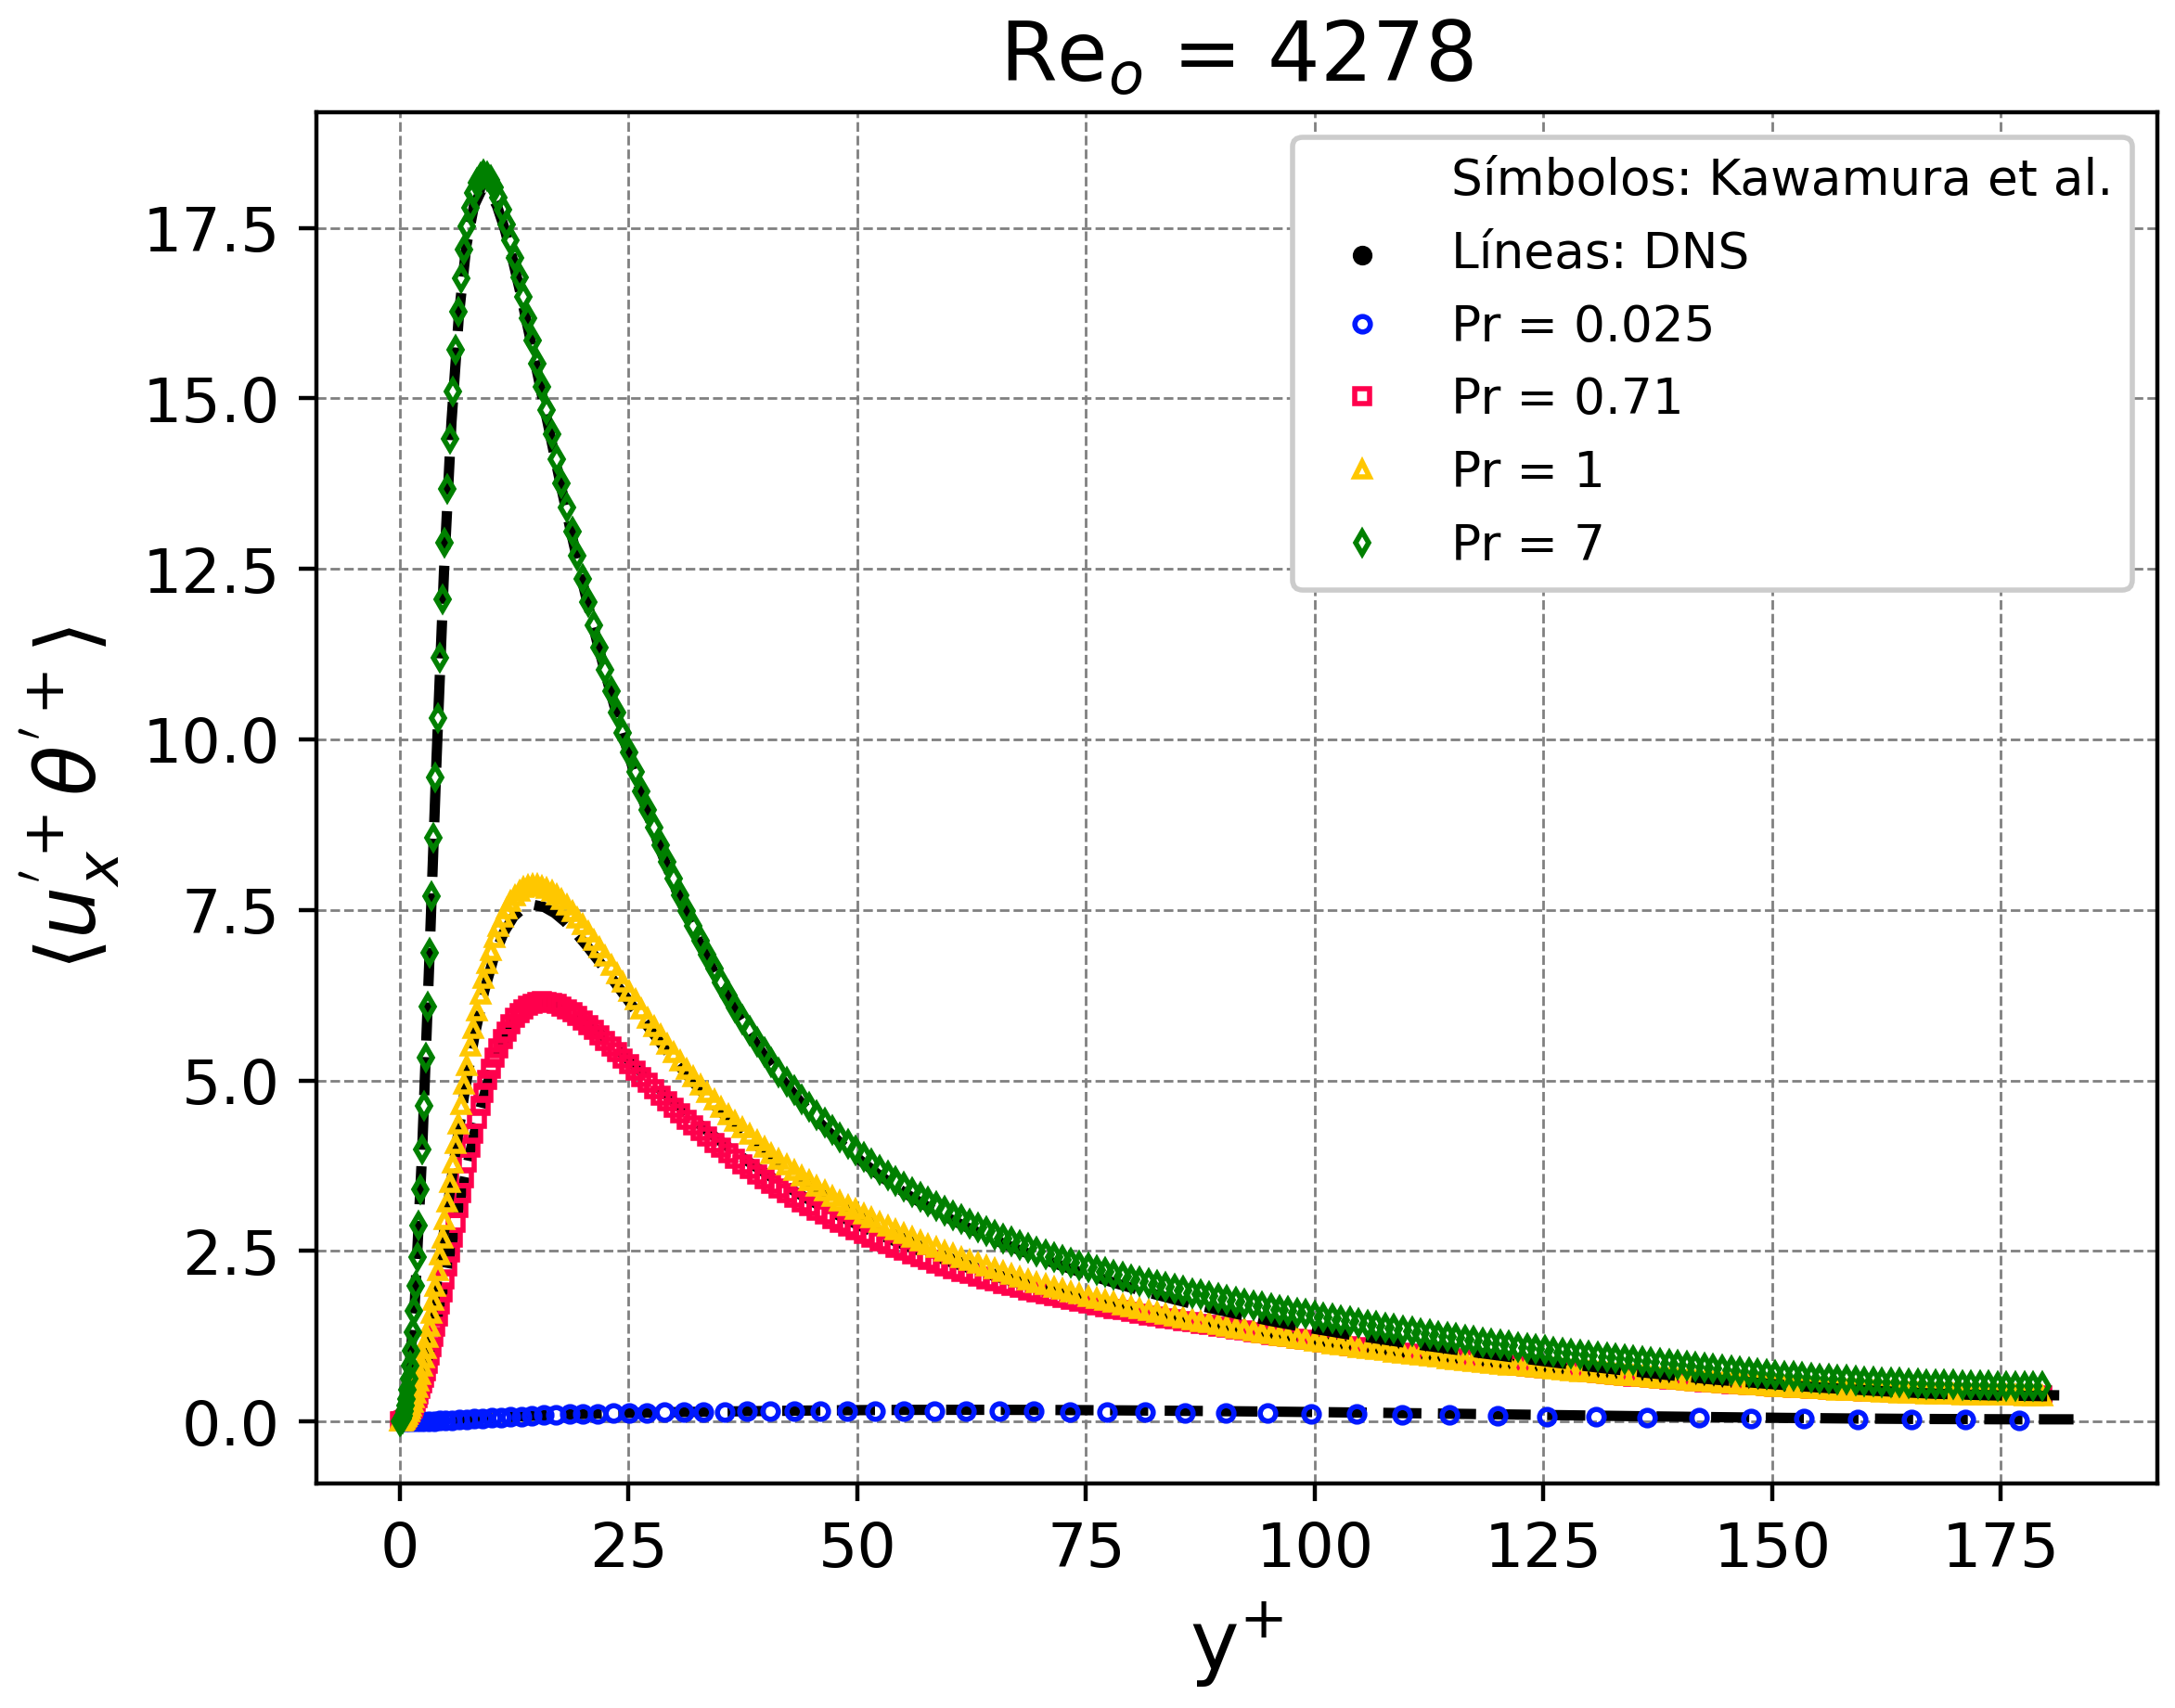
\includegraphics[width=0.49\textwidth]{figures/cap4/kawamura_prs/tep_up_thetap.png}
    \label{fig:kpr-ux-theta}}  
    \subfloat[]{
    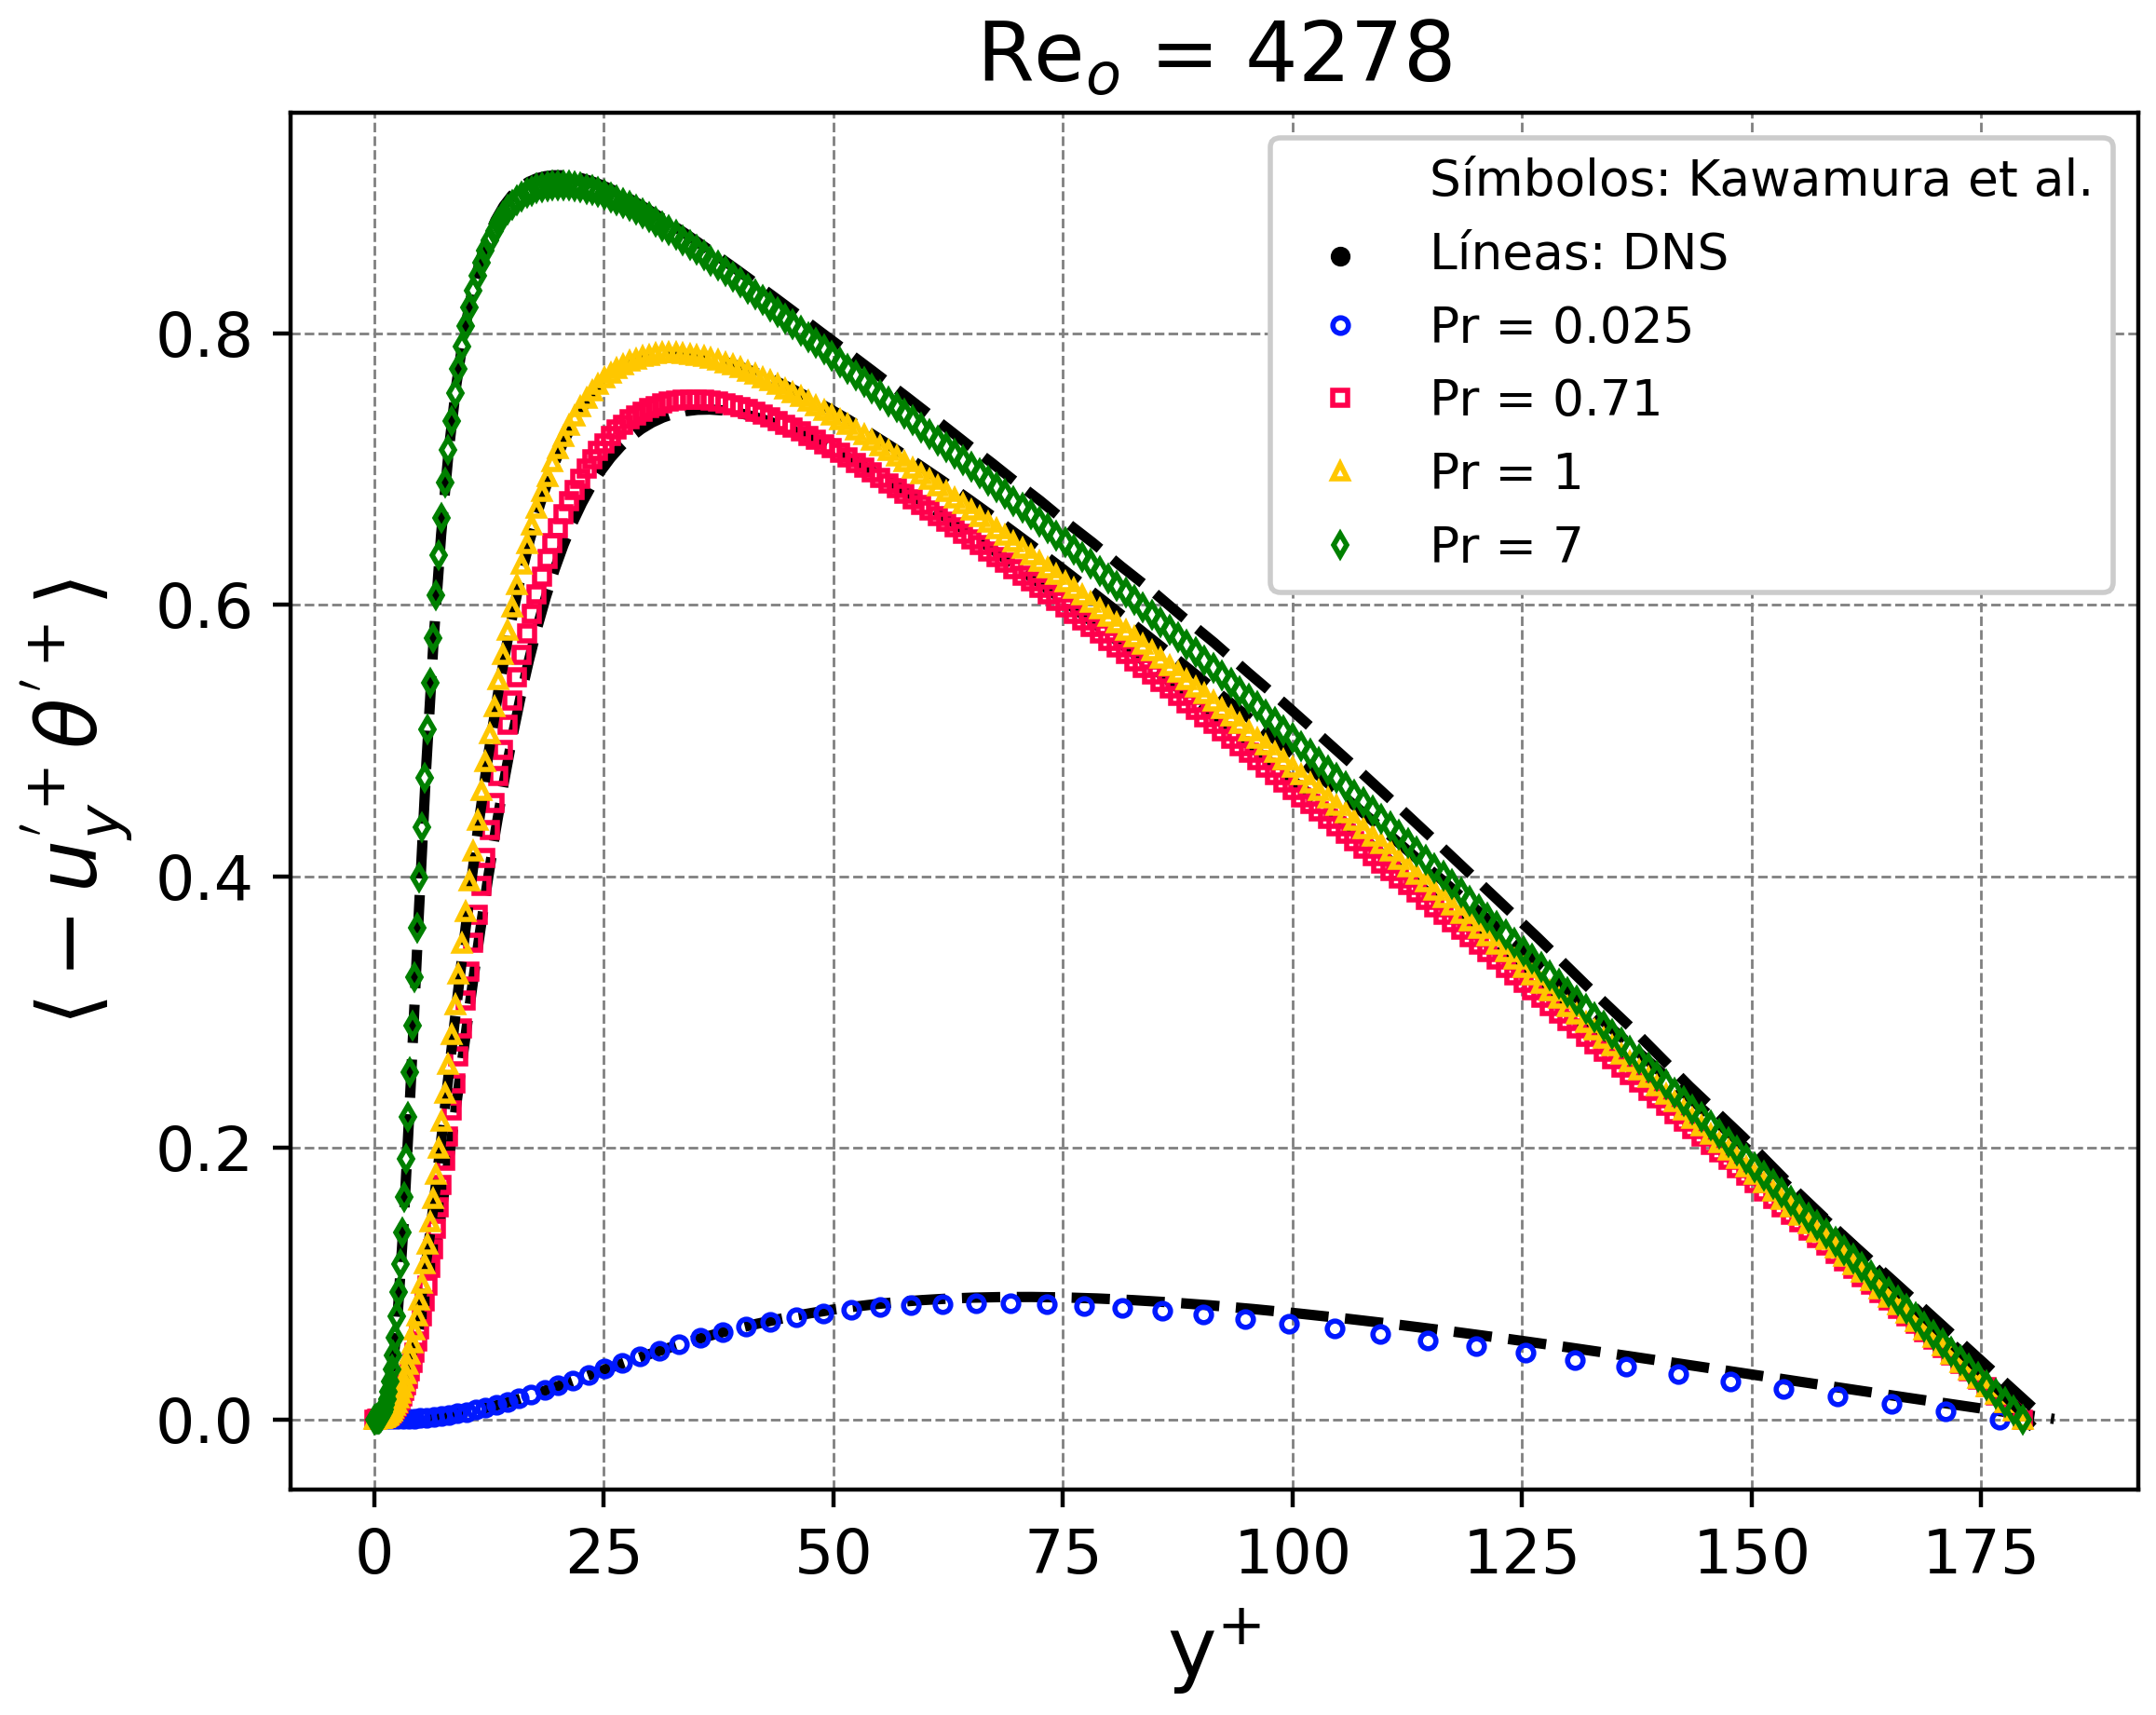
\includegraphics[width=0.49\textwidth]{figures/cap4/kawamura_prs/tep_vp_thetap.png}
    \label{fig:kpr-uy-theta}}  
 \caption{Para diferentes números de Pr se tiene los perfiles de \textbf{(a)} temperatura adimensional media, \textbf{(b)} fluctuaciones RMS de la temperatura adimensional, \textbf{(c)} flujo de calor turbulento en la dirección X, $\langle u^+_x \theta^+ \rangle$, y \textbf{(d)} flujo de calor turbulento en la dirección Y, $\langle u^+_y \theta^+ \rangle$.} 
 \label{fig:kpr_1}
\end{figure}


\subsection{Situación III. Canal turbulento en régimen laminar con convección mixta y $q''_w$ constante} \label{sec:mix-laminar}

Hasta aquí, la herramienta numérica XC3D se ha validado en aspectos hidrodinámicos y térmicos bajo convección forzada. Como punto de partida hacia el régimen de convección mixta, se realizan simulaciones considerando un régimen laminar con Re$_o$=100, Pr=1 y distintos números de Rayleigh (Ra = -25, -100, 75, 150, 250) a fin de evaluar el desempeño de XC3D frente a la influencia de la fuerza boyante. En todas las simulaciones se utiliza la malla M0. A diferencia de los apartados anteriores, en estas simulaciones no se impone ninguna condición adicional en el flujo con la intención de acelerar el paso al régimen turbulento ya que estamos tratando con soluciones laminares.

Se comparan los perfiles de velocidad \textit{streamwise} y de temperatura adimensional con las soluciones analíticas de Chen y Chung \cite{chen1996linear}, dadas por las ecuaciones \ref{eq:vel_asist_boyant} - \ref{eq:theta_opo_boyant}. Los mismos se encuentran en la forma adimensional descrita en el Capítulo \ref{cap:modelo}. En las Figuras \ref{fig:chen-ux} y \ref{fig:chen-theta}, las soluciones analíticas se muestran con anillos negros; asimismo, se incluye el caso con $\text{Ra}=0$ ($\Pi=0$) como referencia (linea azul a trazos). Se aprecia una excelente concordancia entre las soluciones analíticas y las simulaciones DNS, tanto para flujo descendente ($\text{Ra}<0$) como para flujo ascendente ($\text{Ra}>0$). En consecuencia, la malla M0 (la opción computacionalmente más económica) reproduce con alta fidelidad la soluciones laminares de Chen y Chung. 

\begin{figure}[H]
 \centering
  \subfloat[]{
    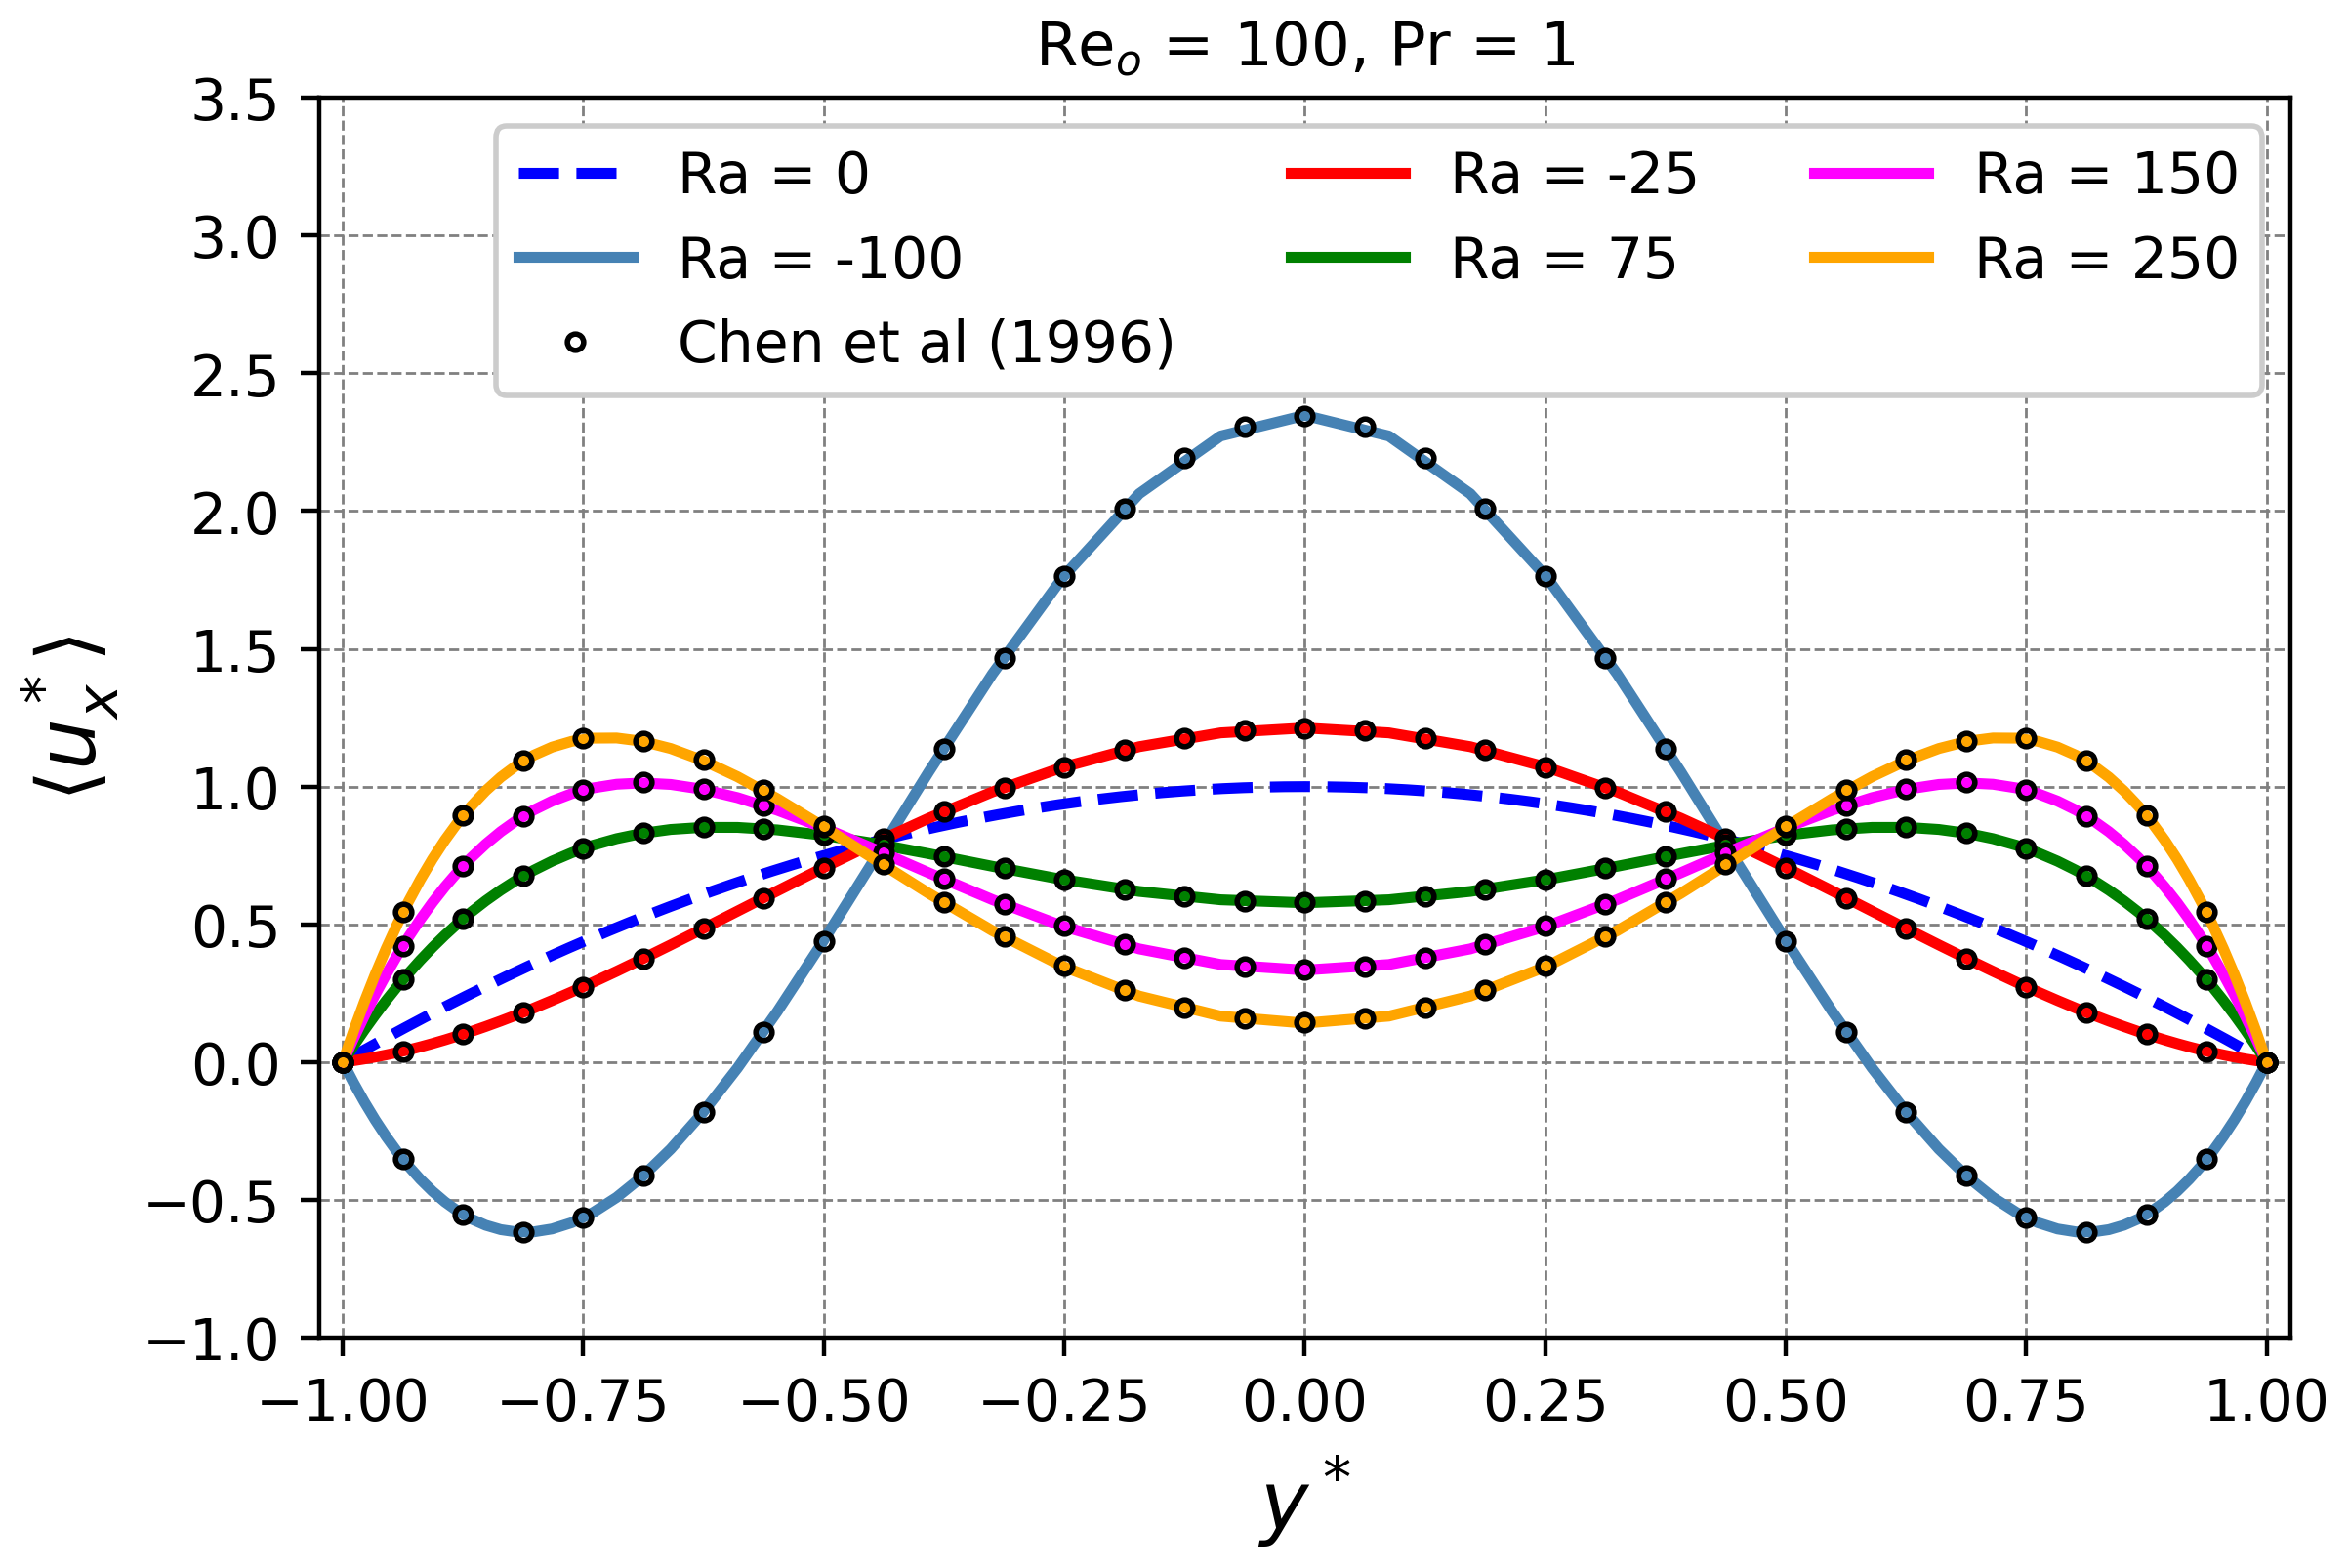
\includegraphics[width=0.5\textwidth]{figures/cap4/laminar/ux_mean.png}
    \label{fig:chen-ux}}  
    \subfloat[]{
    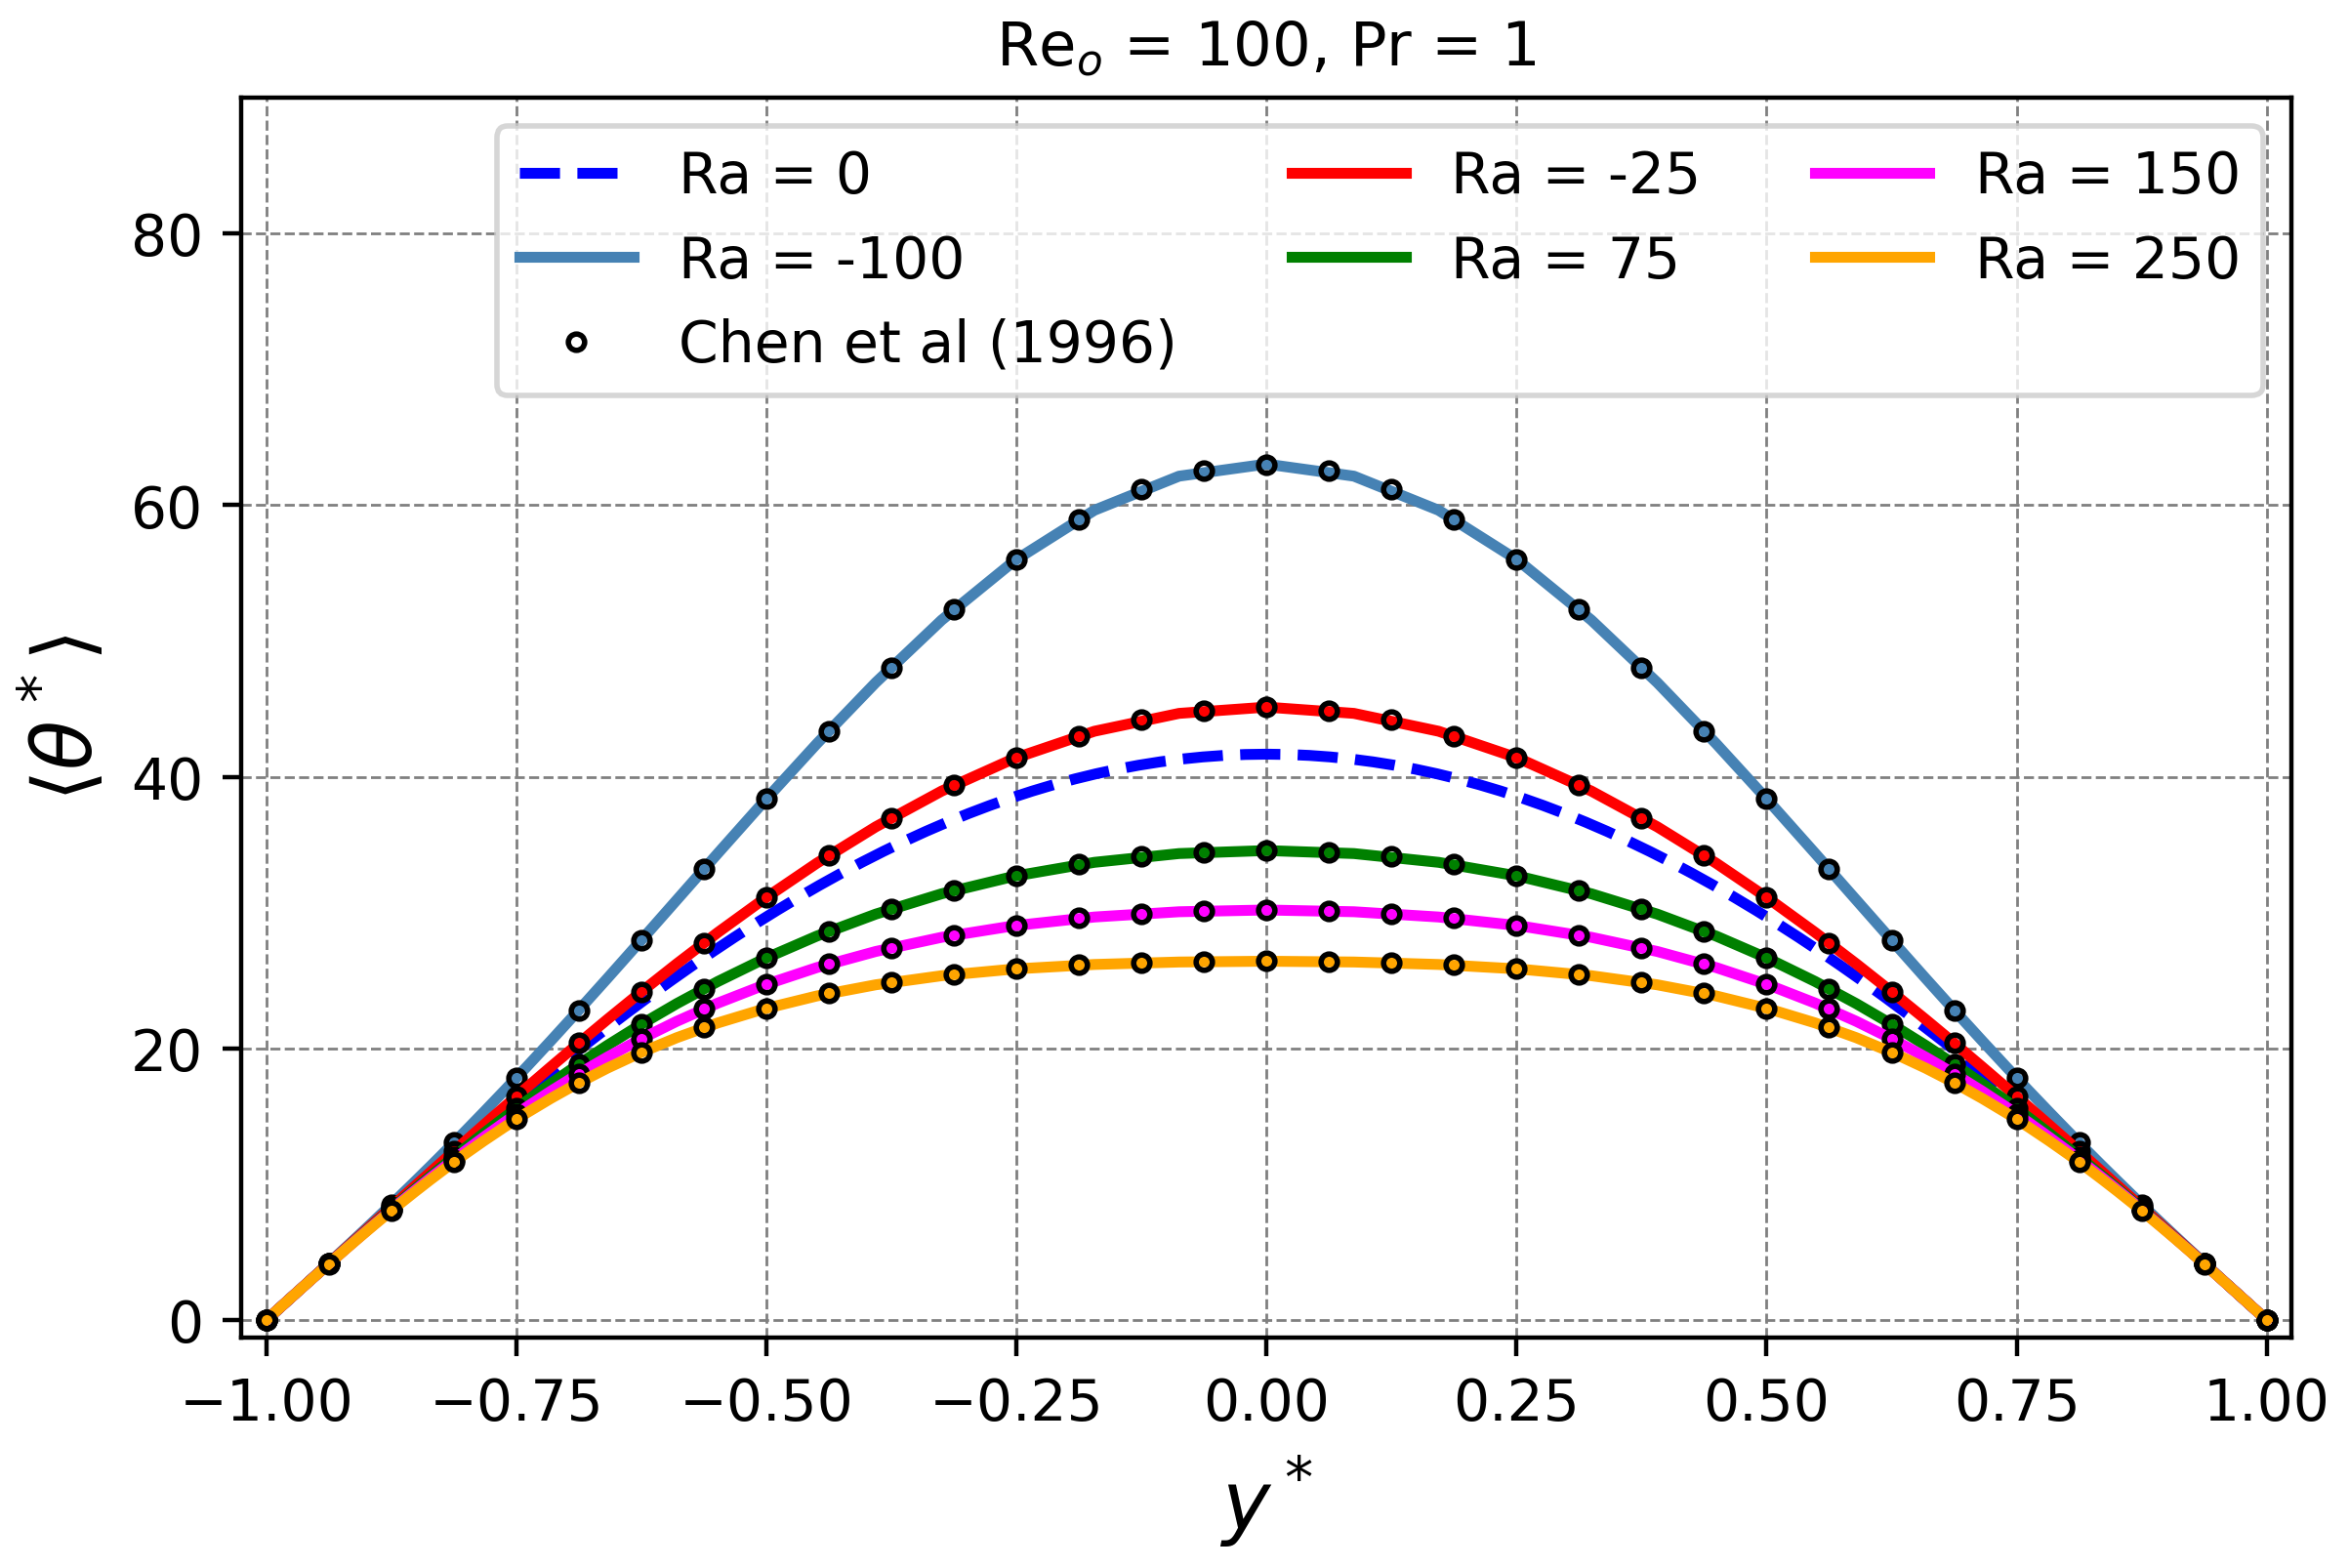
\includegraphics[width=0.5\textwidth]{figures/cap4/laminar/theta_mean.png}
    \label{fig:chen-theta}}  
 \caption{Perfiles de velocidad y temperatura para distintos casos en régimen laminar con convección mixta.} 
 \label{fig:chen-profiles}
\end{figure}


\subsection{Situación IV. Canal turbulento en convección mixta con $\Delta T$ constante entre paredes.}

\textit{Observación inicial: en el momento que se realizaron las simulaciones para validar la implementación del término de fuerza boyante en XC3D, no se encontraba disponible en la bibliografía de ese momento, datos de referencia en canales rectangulares para flujo turbulento con régimen de convección mixta ascendente (o descendente) con flujo de calor impuesto en las paredes. La única alternativa disponible era el trabajo de Guo \textit{et al.} \cite{guo2022direct} basado en un sistema físico conceptualmente diferente, con paredes isotérmicas a distinta temperatura en lugar de flujo de calor impuesto. Más recientemente, en 2024, Zhou \textit{et al.} publicaron un \textit{paper} \cite{zhou2024direct} con datos de simulaciones DNS para del mismo sistema físico considerado en este trabajo.} 



\begin{figure}[H]
 \centering
  \subfloat[]{
    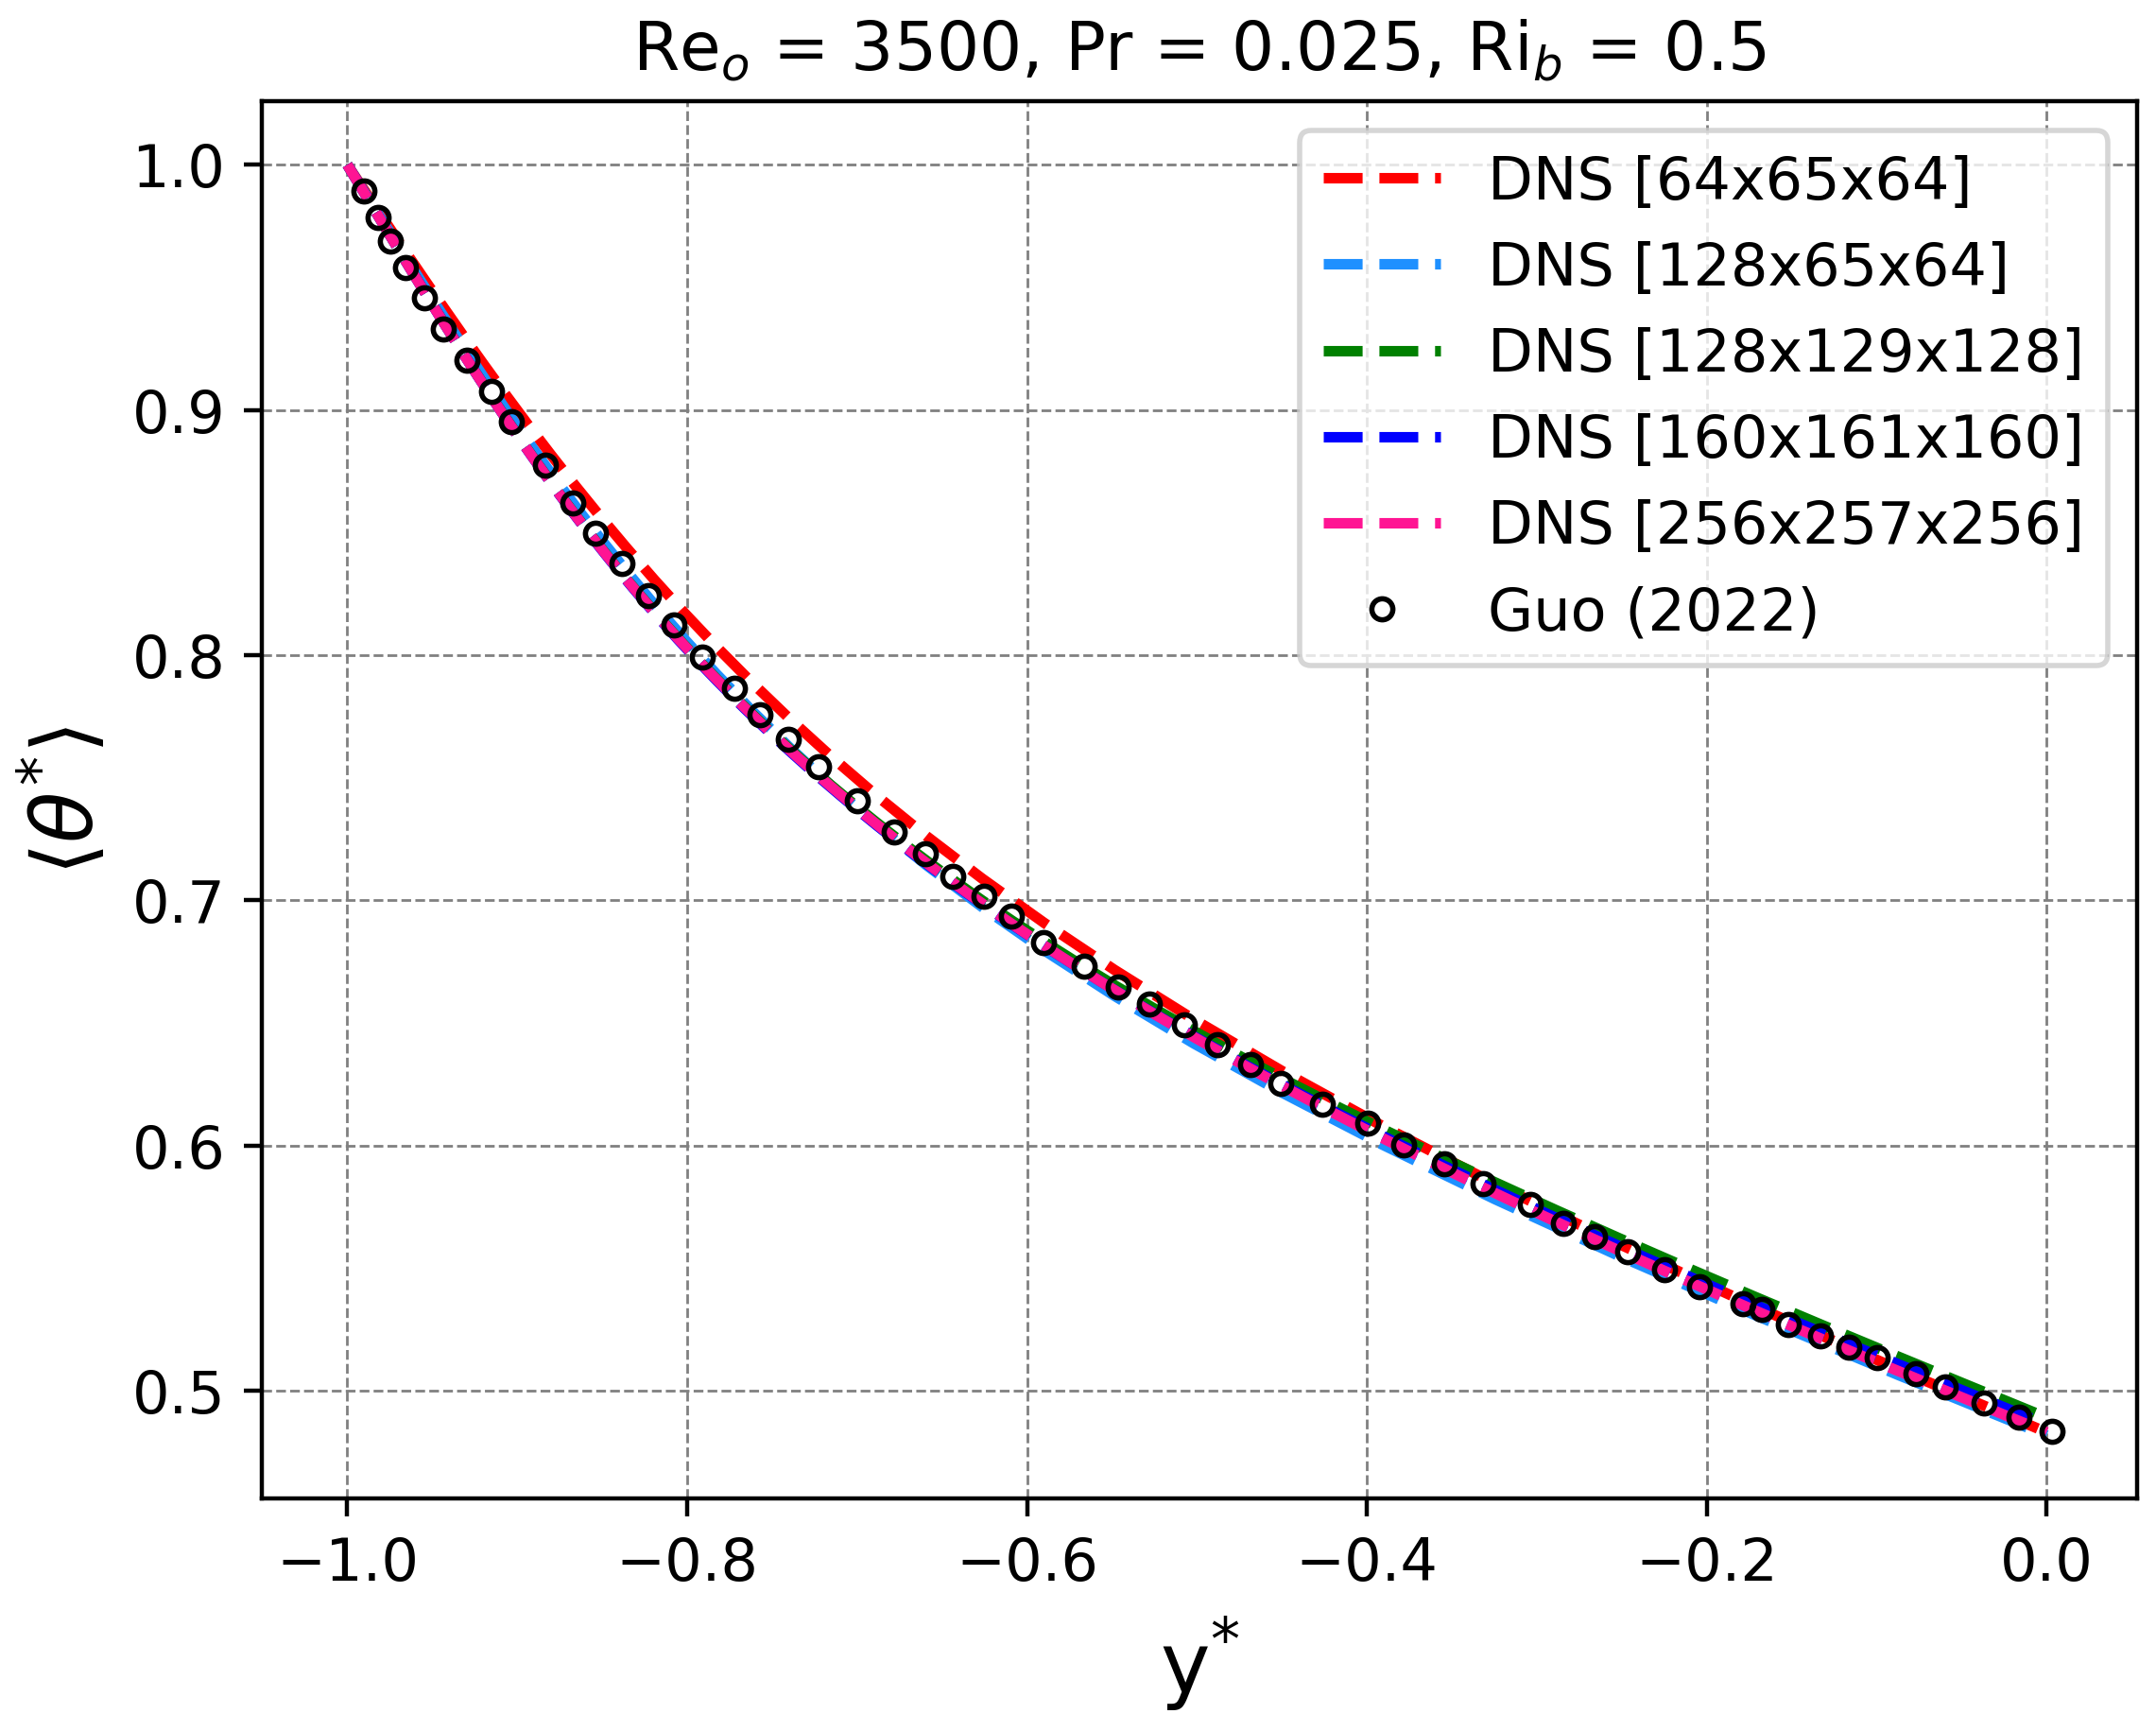
\includegraphics[width=0.49\textwidth]{figures/cap4/guo/Rib05/mct_theta.png}
   		\label{fig:guo-05-theta}}  
    \subfloat[]{
    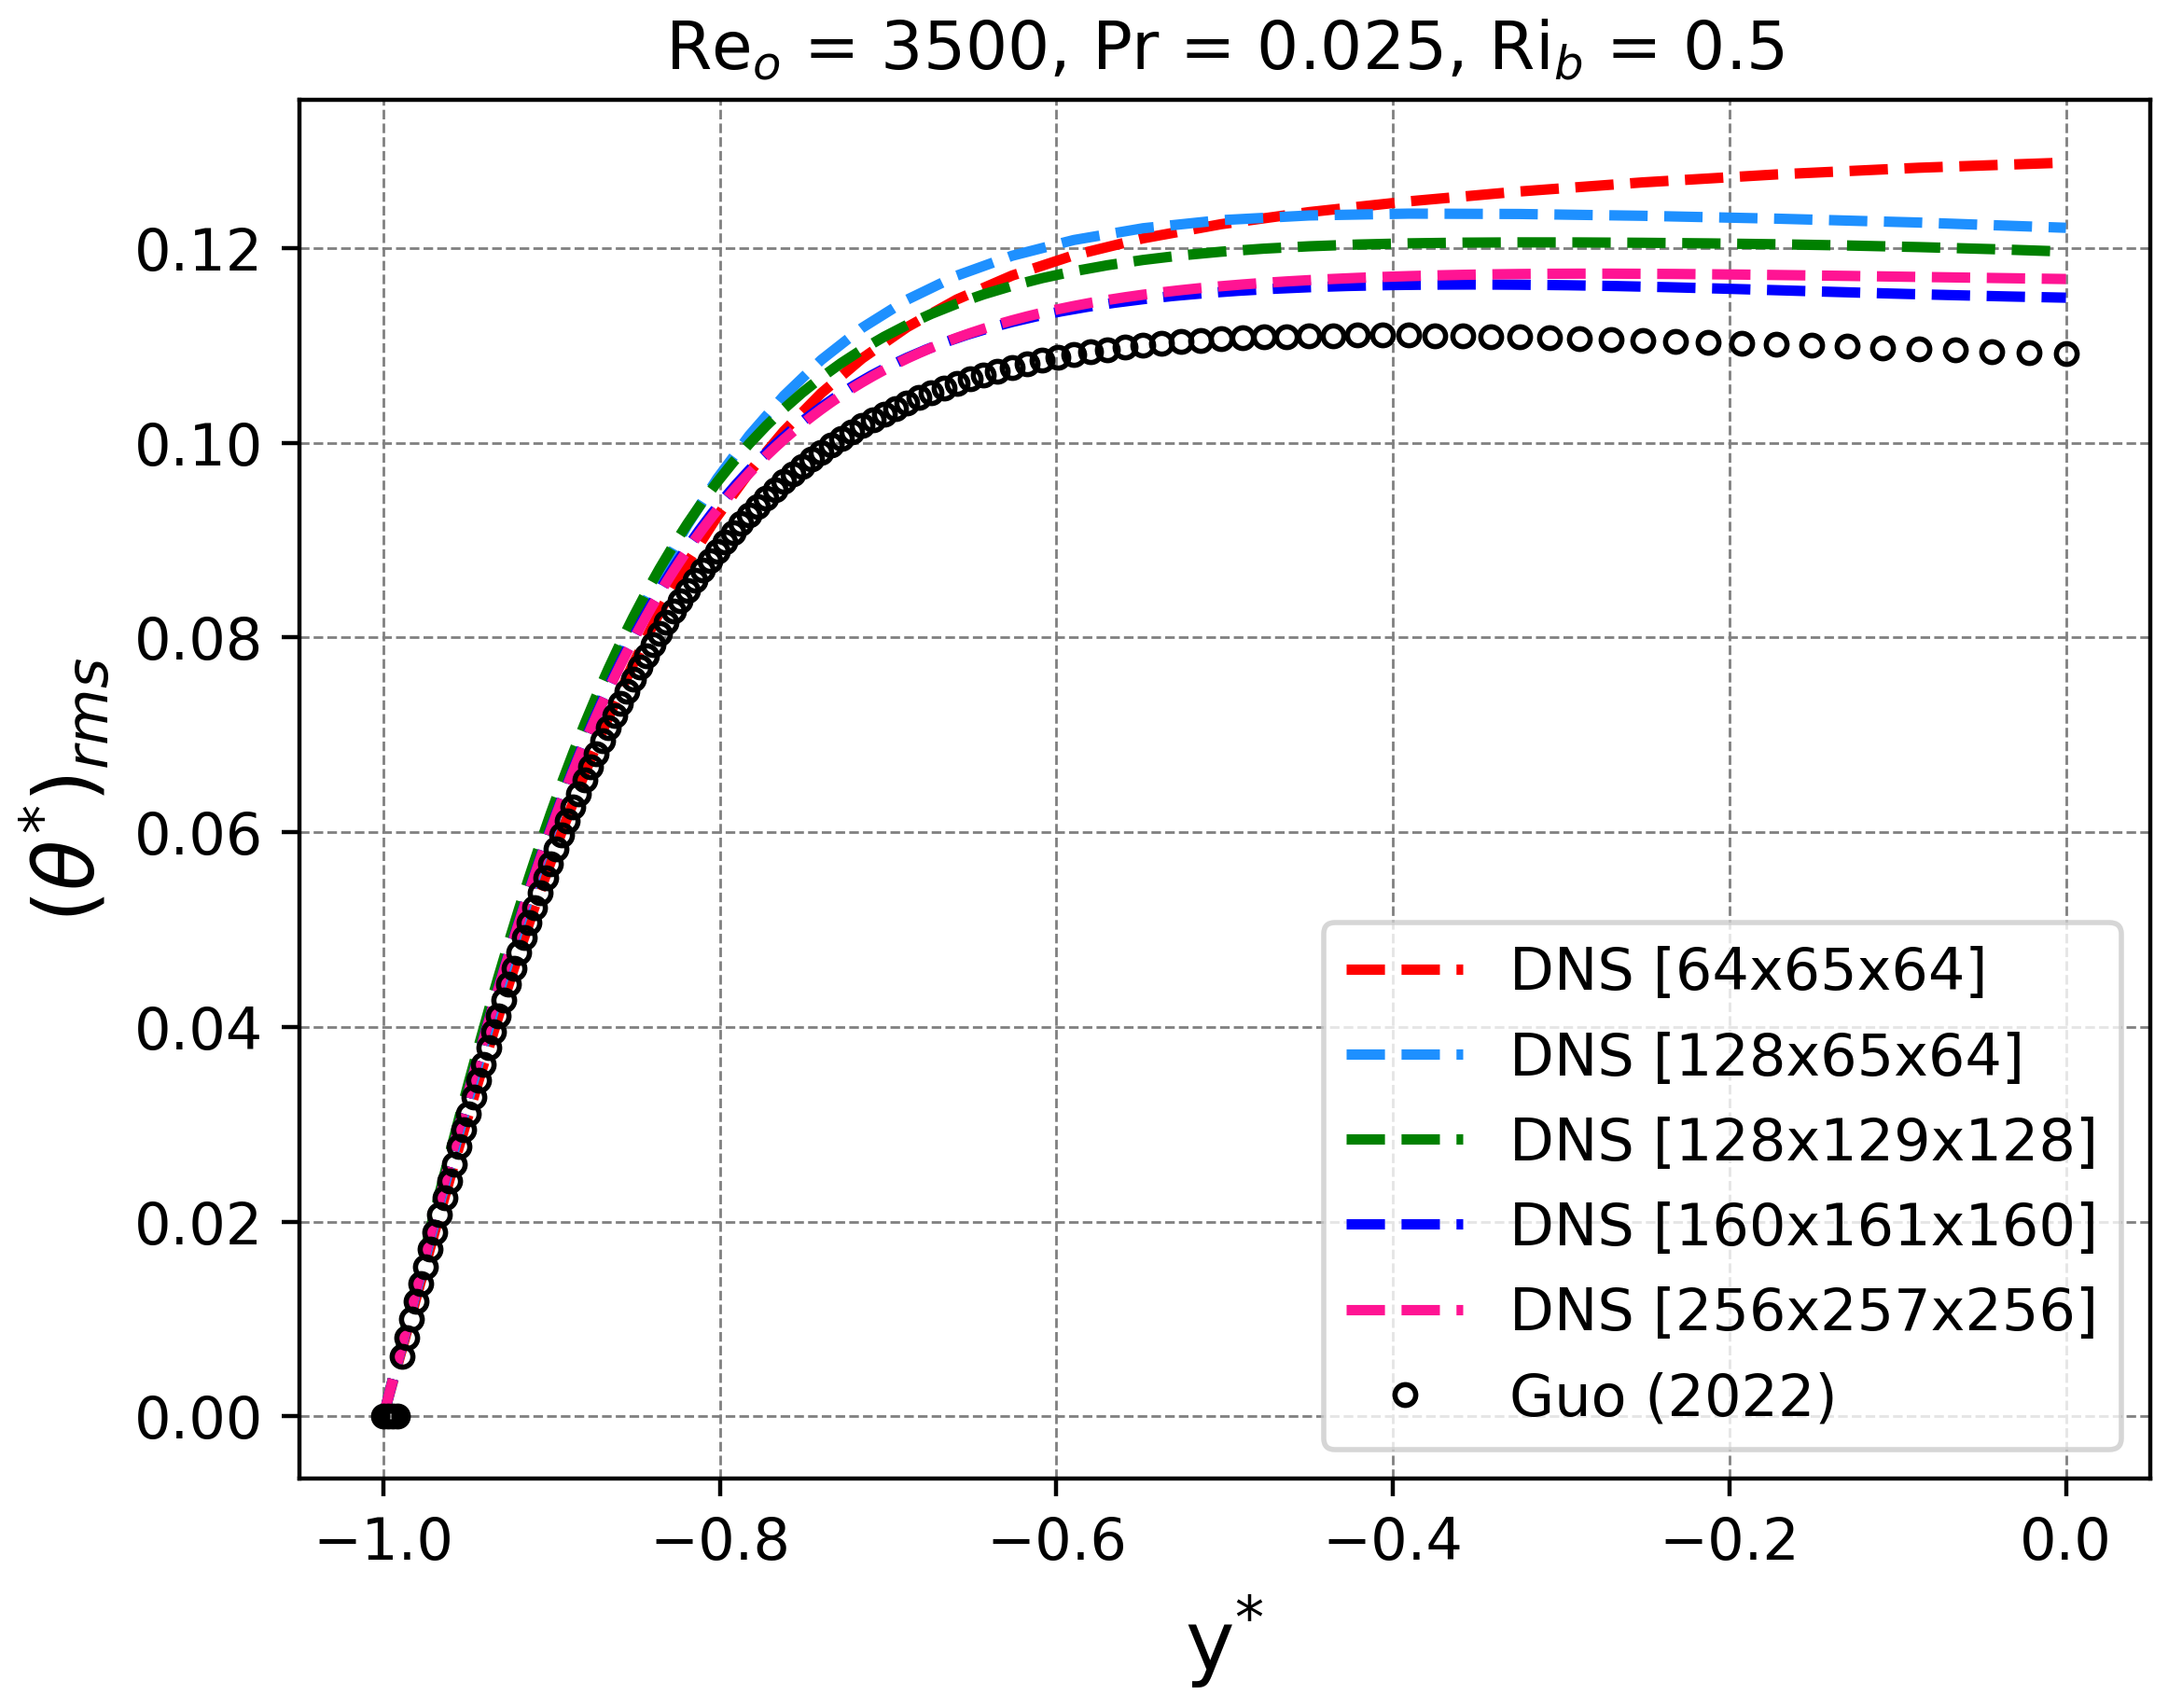
\includegraphics[width=0.49\textwidth]{figures/cap4/guo/Rib05/mct_thetap_rms.png}
  		\label{fig:guo-05-theta-rms}}  

  \subfloat[]{
    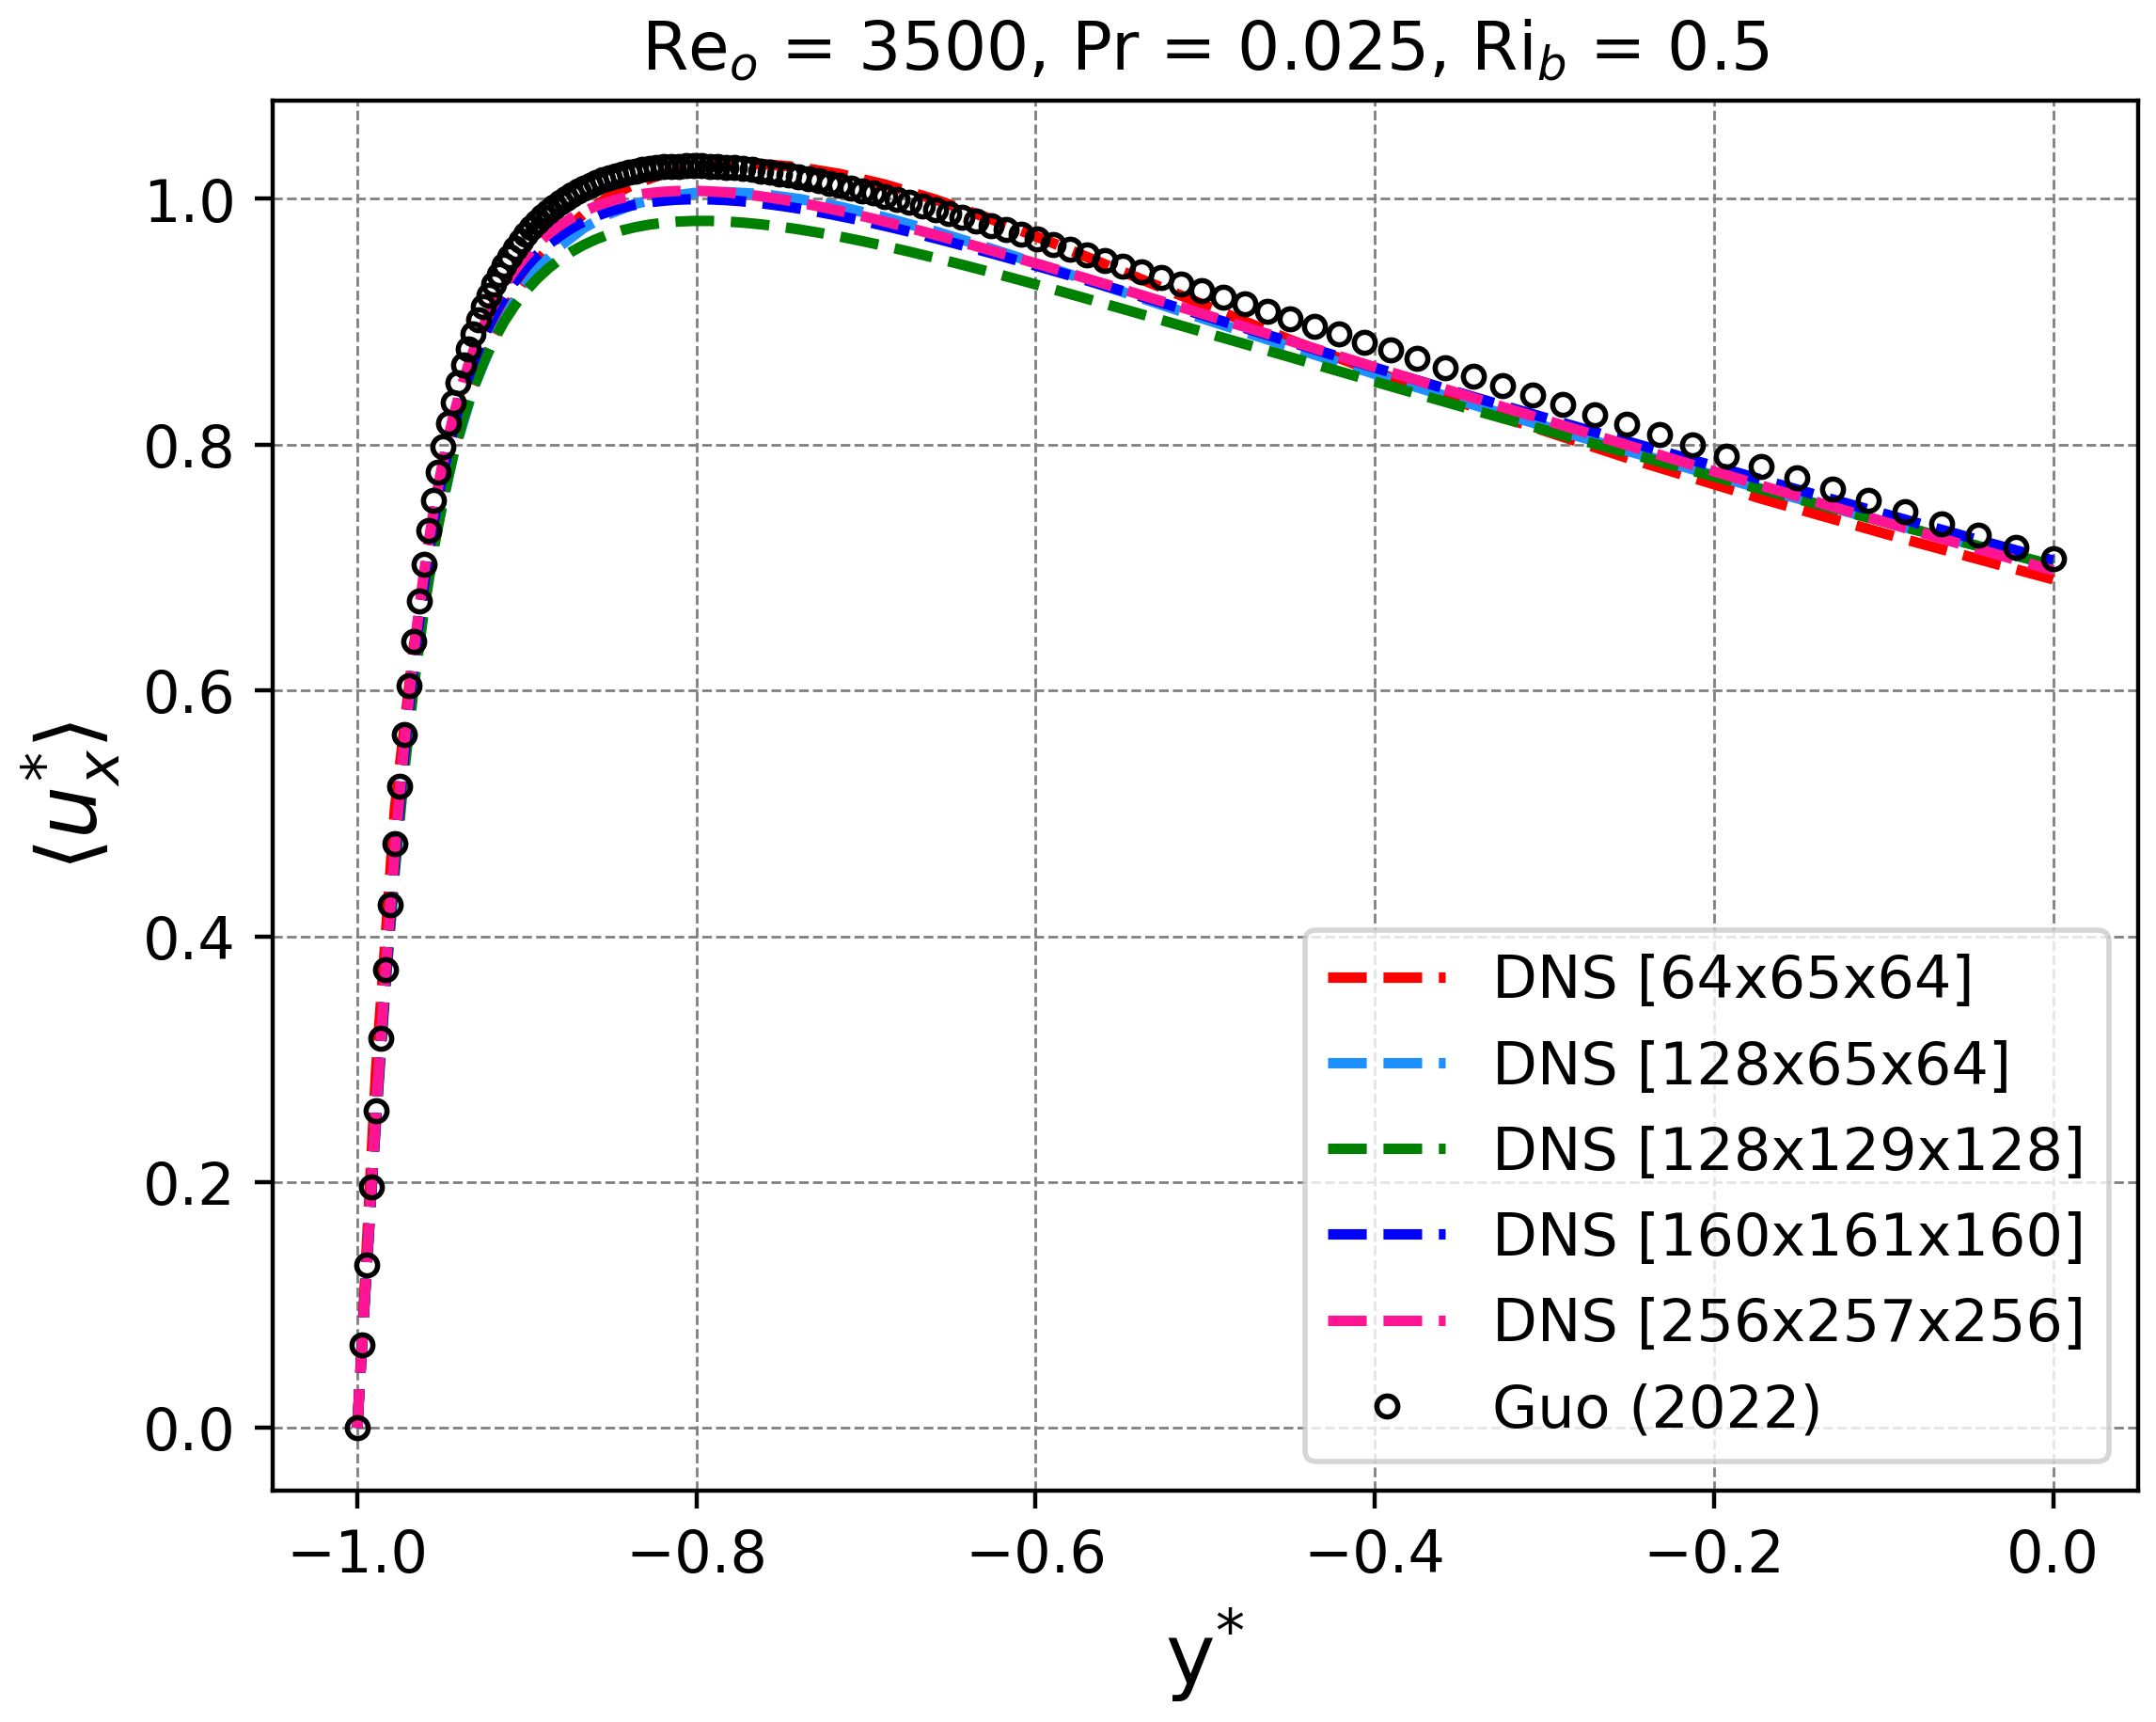
\includegraphics[width=0.49\textwidth]{figures/cap4/guo/Rib05/mct_upmean.png}
   		\label{fig:guo-05-ux}}  
    \subfloat[]{
    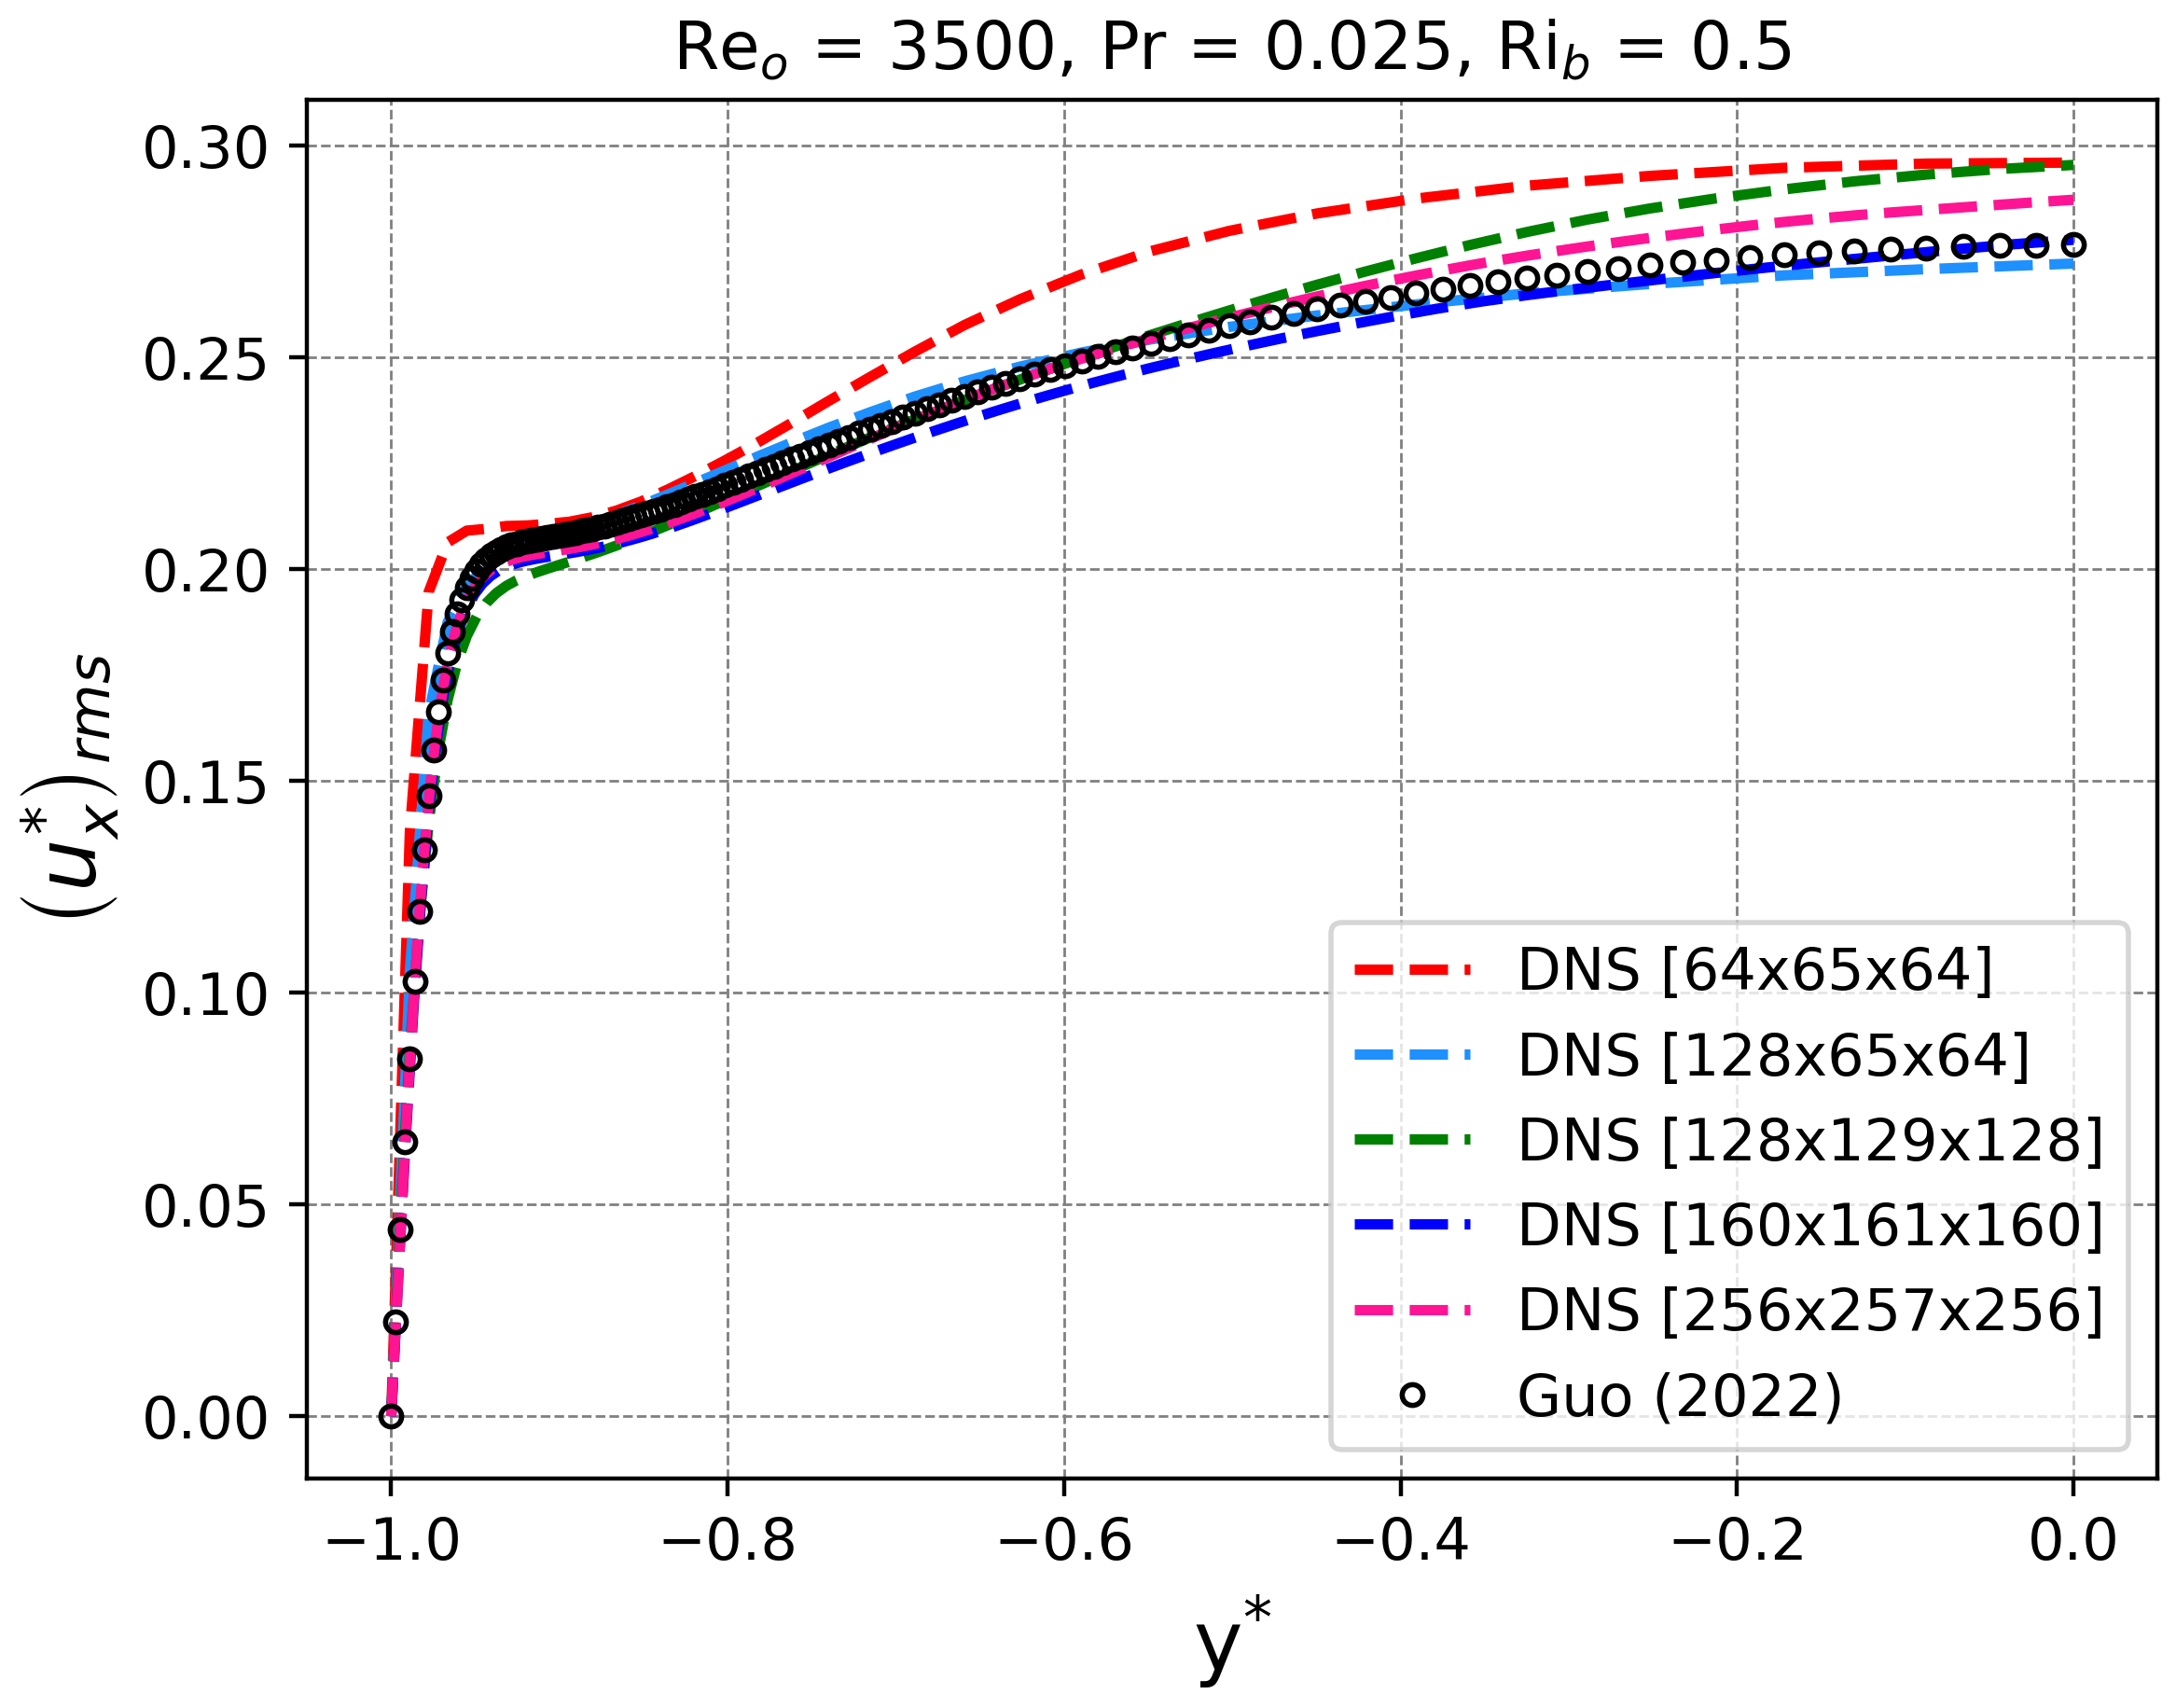
\includegraphics[width=0.49\textwidth]{figures/cap4/guo/Rib05/mct_uprms.png}
    	\label{fig:guo-05-ux-rms}}  

  \subfloat[]{
    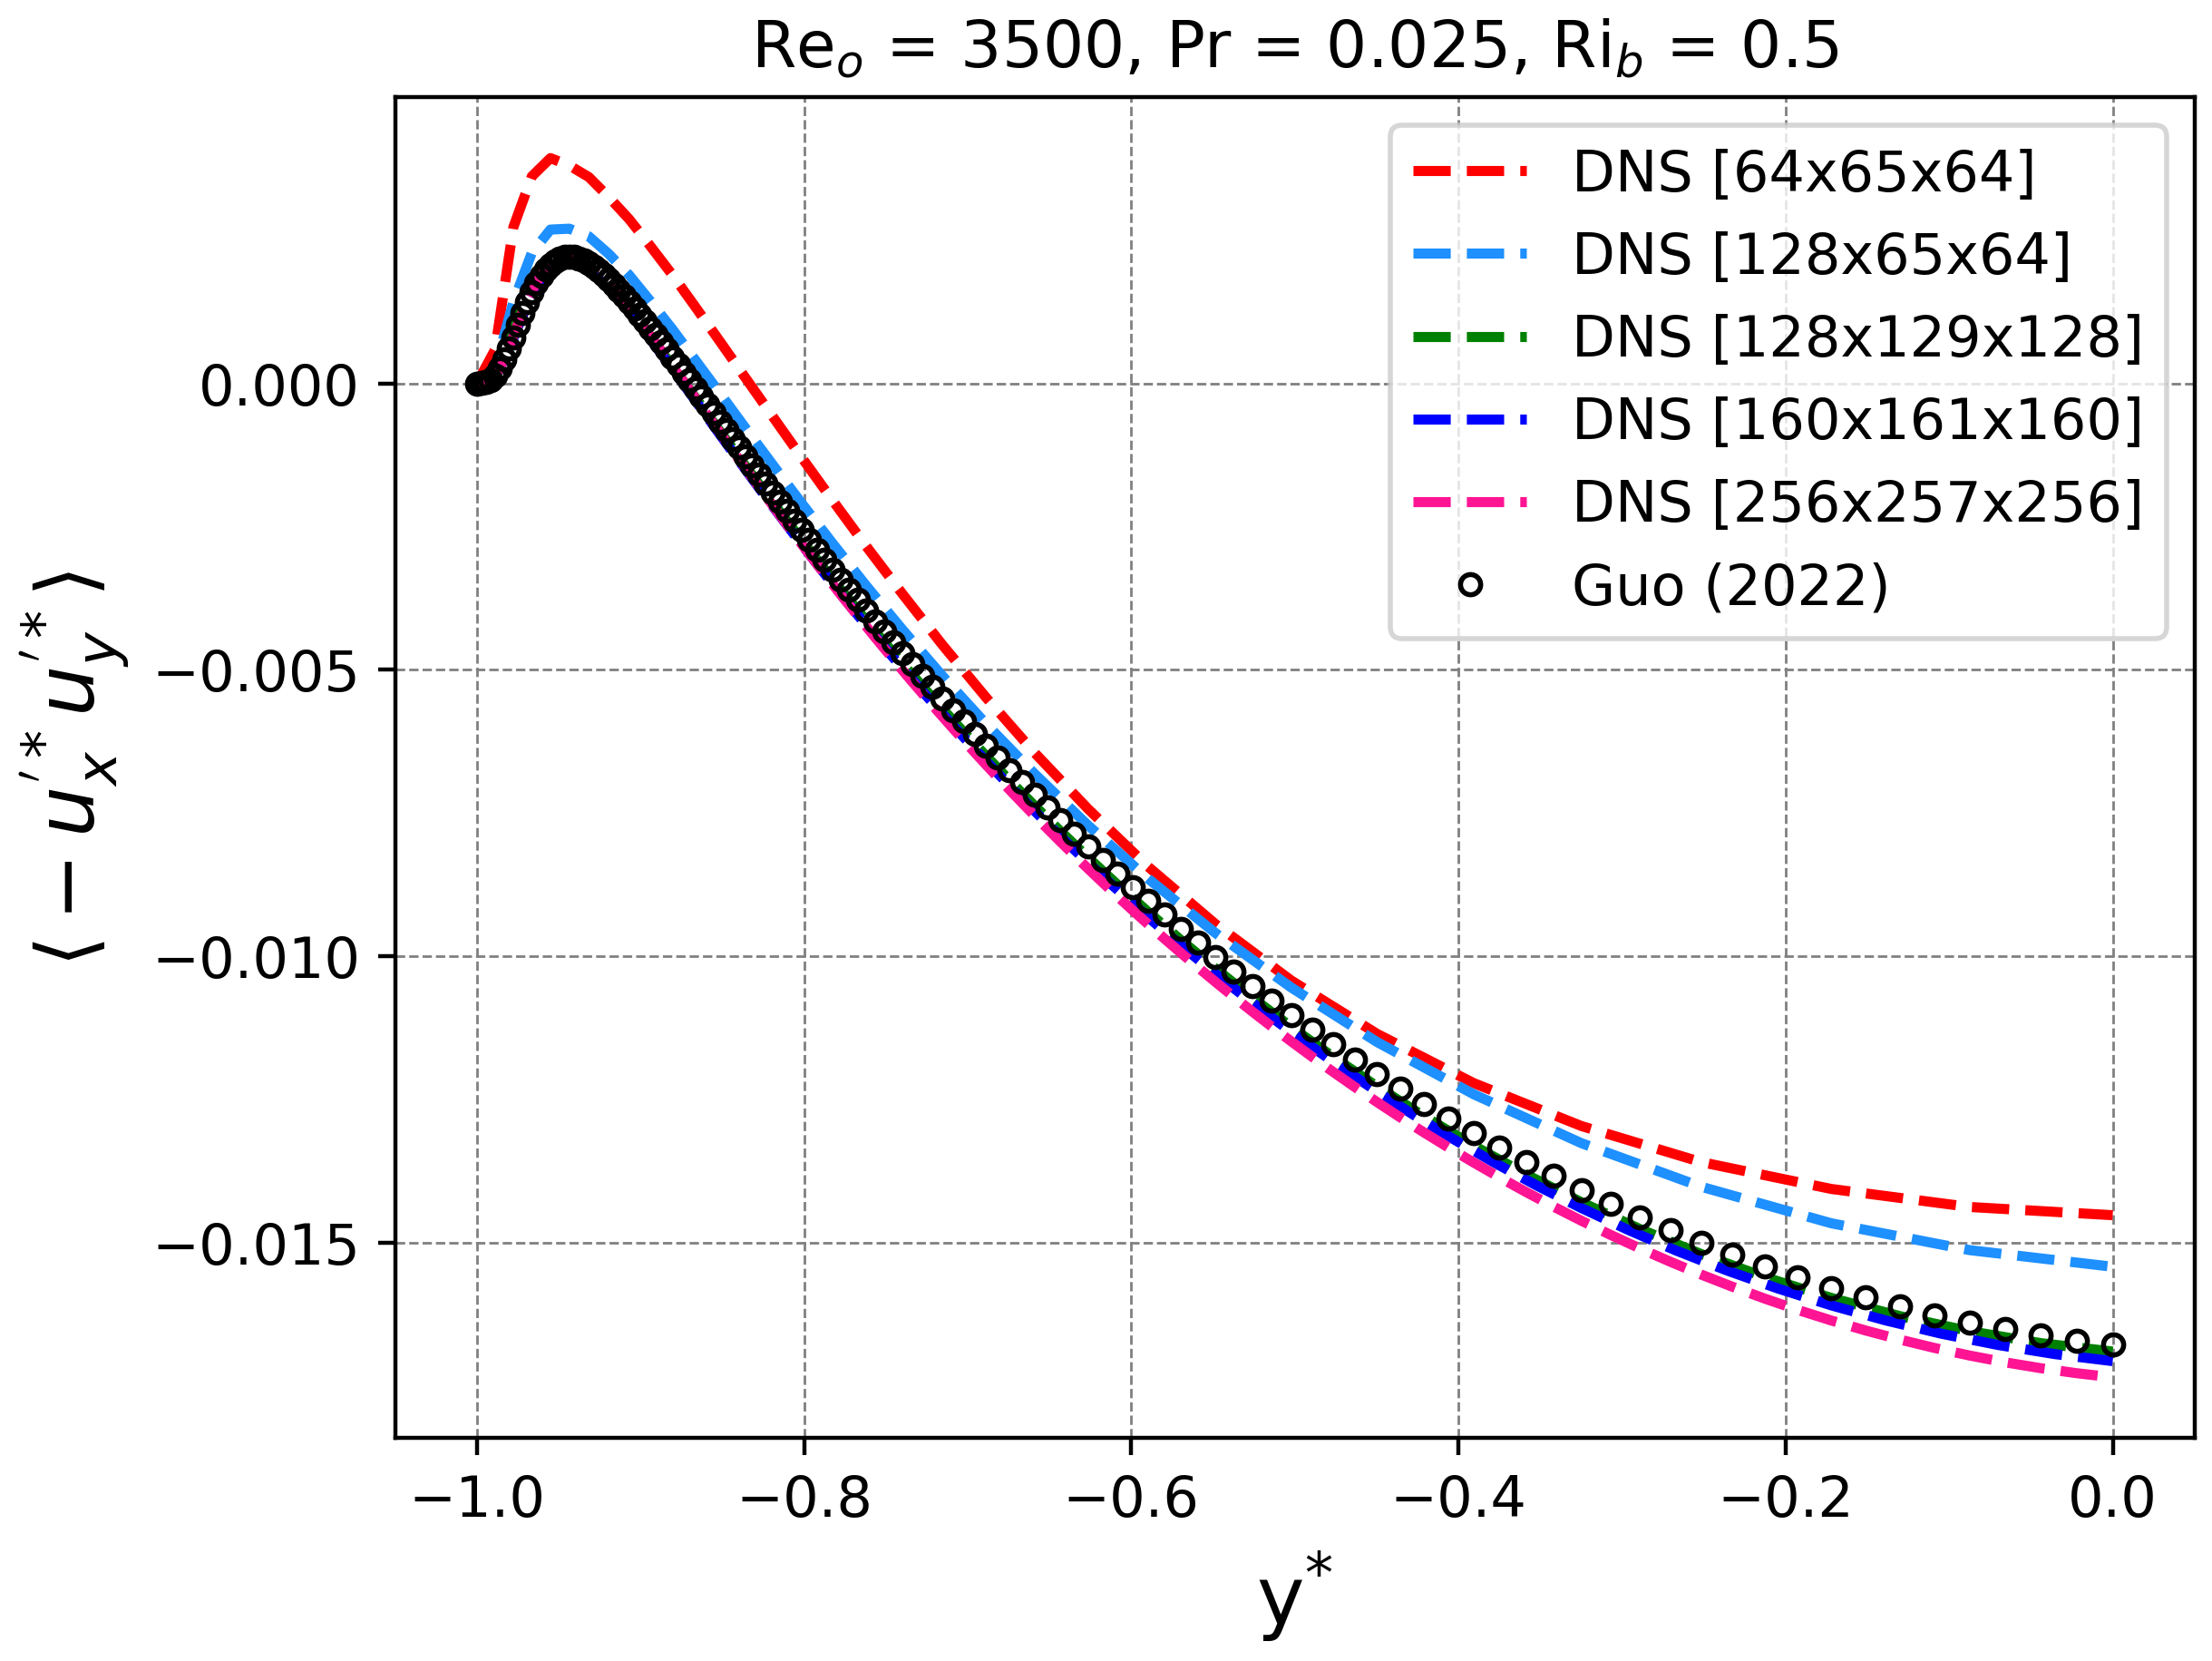
\includegraphics[width=0.49\textwidth]{figures/cap4/guo/Rib05/mct_up_vp.png}
    	\label{fig:guo-05-uxuy}}  
    \subfloat[]{
    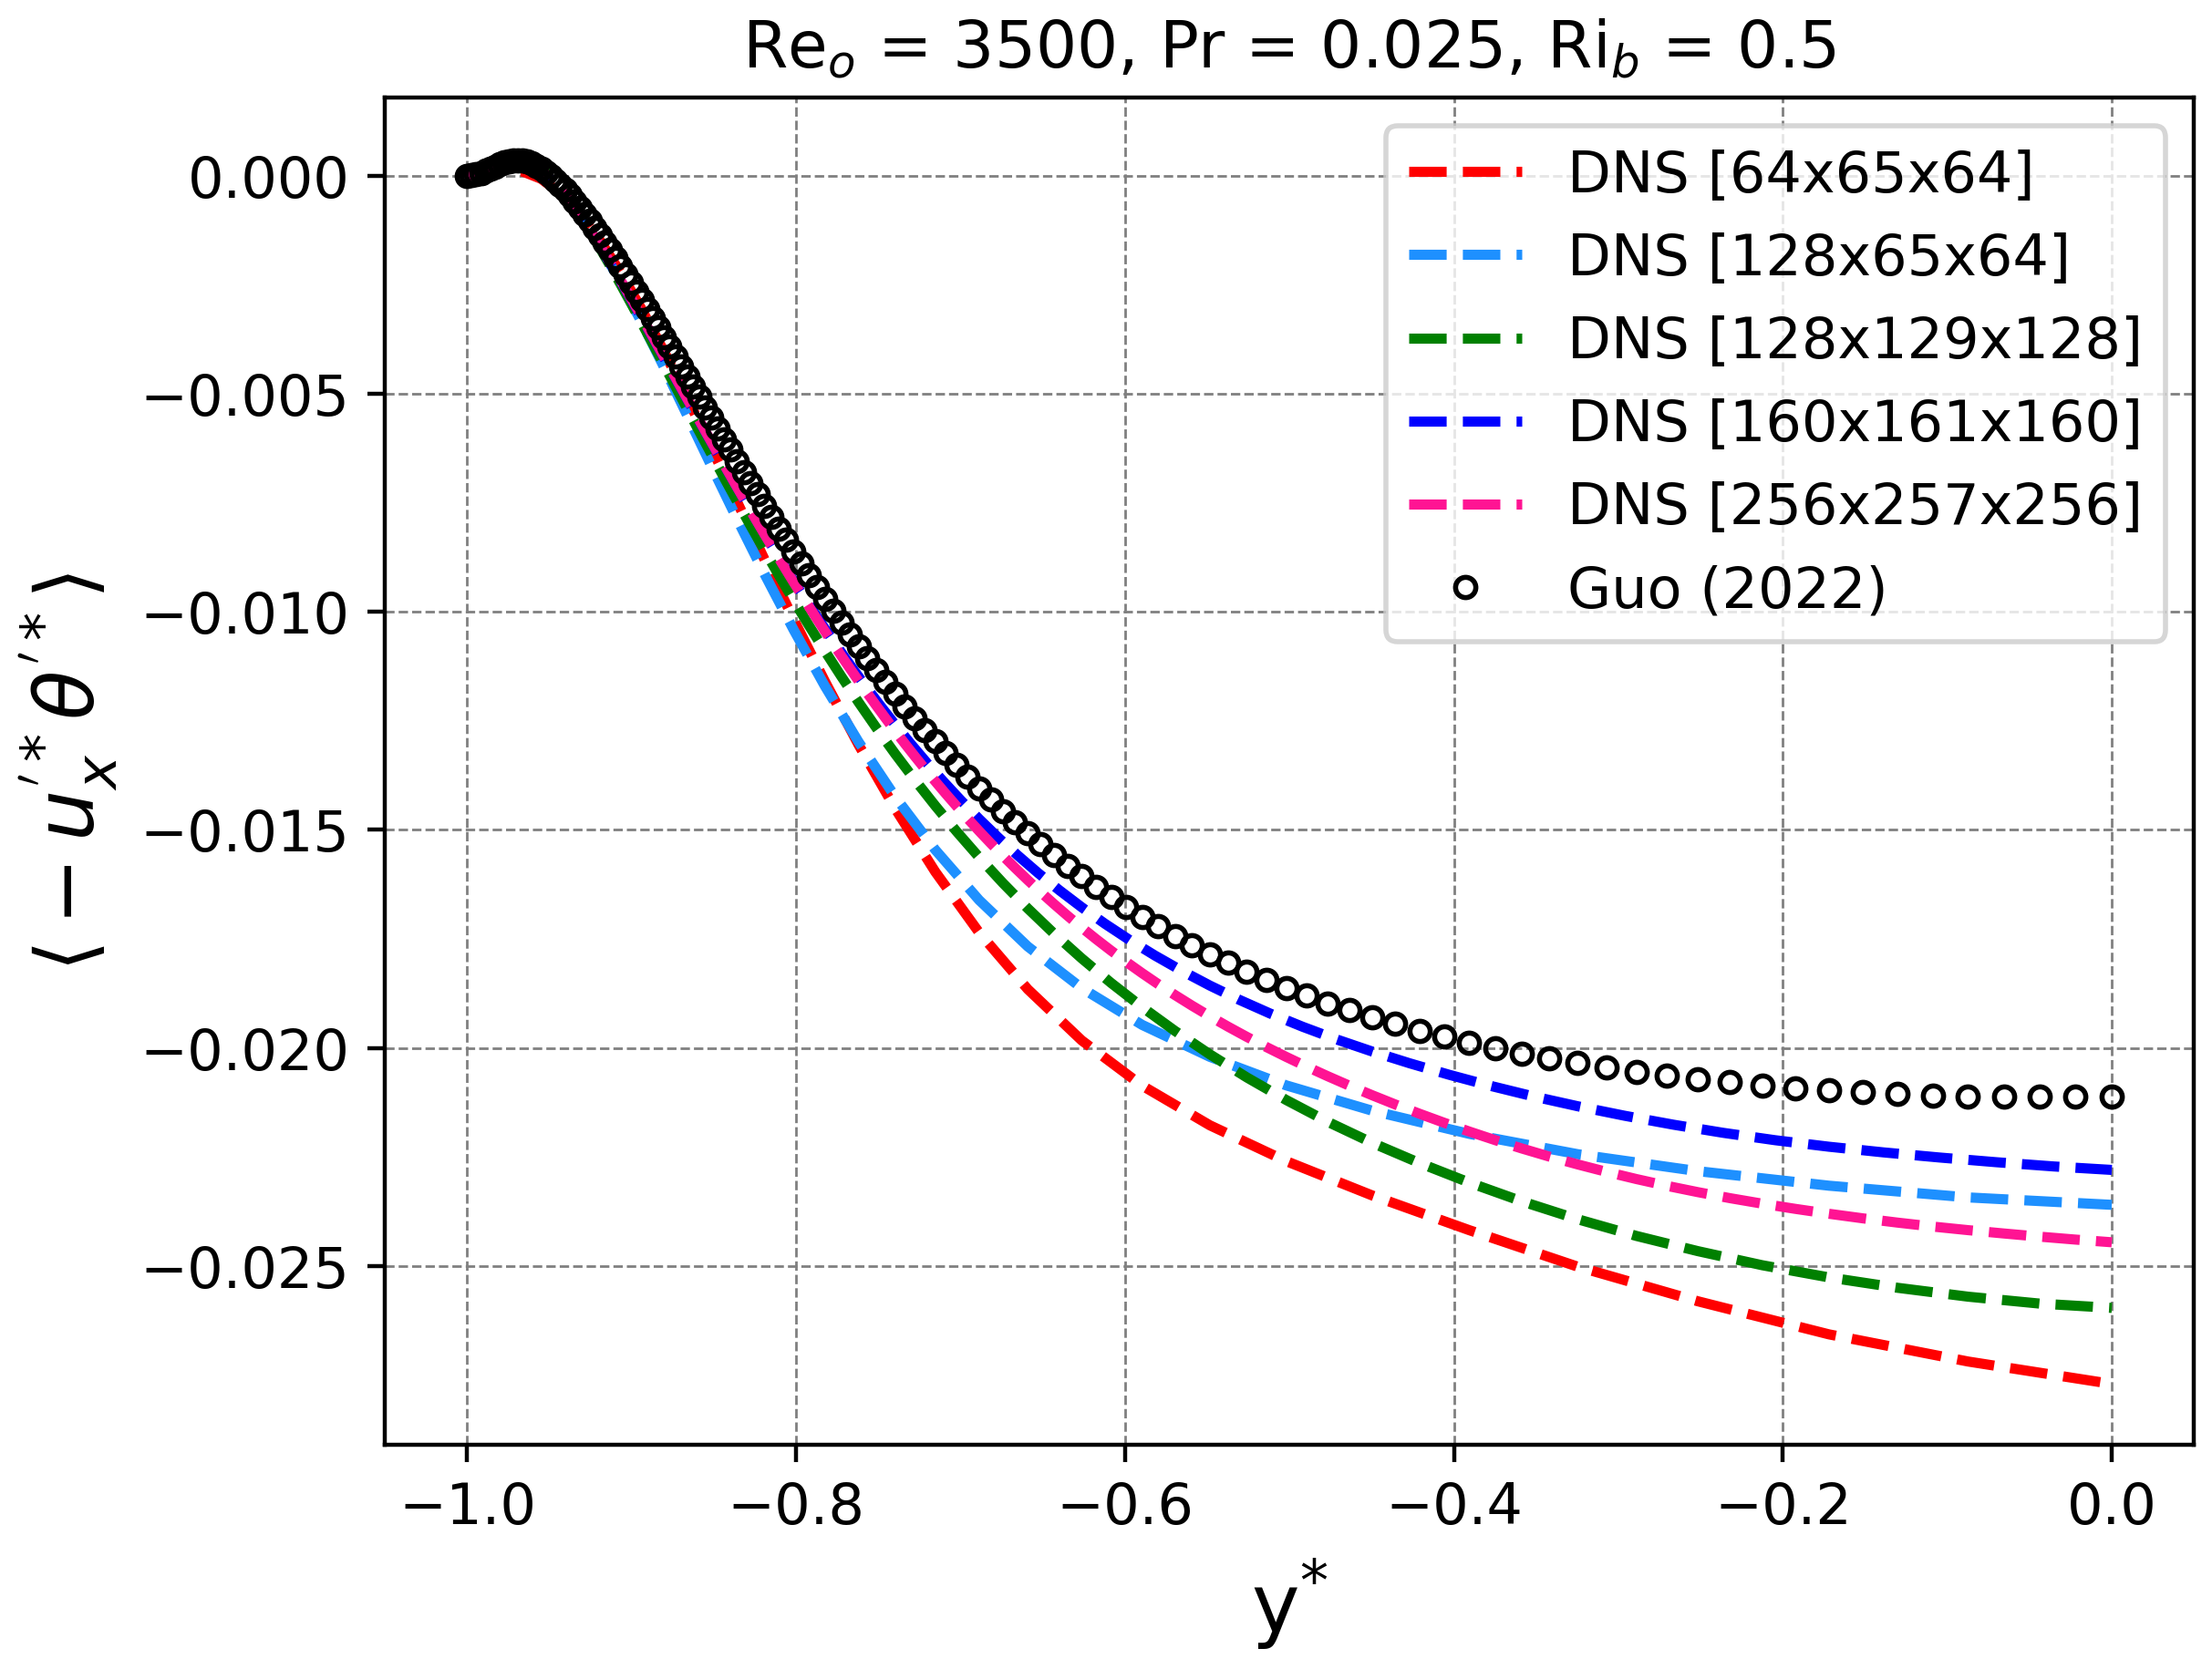
\includegraphics[width=0.49\textwidth]{figures/cap4/guo/Rib05/mct_up_thetap.png}
    	\label{fig:guo-05-ux-theta}}  
 \caption{Perfiles de \textbf{(a)} temperatura adimensional media, \textbf{(b)} fluctuaciones RMS de la temperatura adimensional, \textbf{(c)} velocidad media \textit{streamwise}, \textbf{(d)} fluctuaciones RMS de la velocidad \textit{streamwise}, \textbf{(e)} componente XY del tensor de Reyndols, $\langle -u^+_x u^+_y \rangle$, y \textbf{(f)} flujo de calor turbulento en la dirección X, $\langle -u^+_x \theta^+ \rangle$.} 
 \label{fig:guo-05}
\end{figure}

Cuando se tiene en cuenta la fuerza boyante, es decir $\Pi \neq 0$, el término asociada a ella en la ecuación de momento produce un acople entre las tres ecuaciones de conservación (ecuaciones \ref{eq:gob_system_adim}) y por lo tanto, la parte hidrodinámica del flujo influye en la parte térmica del mismo y visceversa. 

Se realizan simulaciones empleando las mallas M0 - M4 para analizar su convergencia en malla. En este sentido, se consideran los números adimensionales Re$_o$=3500, Pr=0.025 y Ri$_b$=0.5 para tal fin. Las Figuras \ref{fig:guo-05-theta} - \ref{fig:guo-05-ux-theta} exponen, respectivamente, los perfiles de las siguientes magnitudes: temperatura adimensional, fluctuaciones de temperatura, velocidad \textit{streamwise}, fluctuaciones de velocidad, componente XY del tensor de Reynolds y flujo de calor turbulento en dirección X. Los datos de magnitudes propias se comparan con aquellos datos obtenidos por Guo \textit{et al.} \cite{guo2022direct}. Las mismas se encuentran expresadas en la forma adimnesional: $\mathbf{u^*} = \mathbf{u} / U_b$ y $\theta^* = \theta / \Delta T_{hc}$, siendo $\Delta T_{hc}$ la diferencia de temperatura entre las paredes.

Se aprecia que las magnitudes de primer order, es decir, perfiles de velocidad media y temperatura media, convergen en malla. Por su parte, al comparar magnitudes de segundo orden asociadas a la temperatura adimensional, como la fluctuación de temperatura o el flujo de calor turbulento, se observa una mayor discrepancia entre resultados; por otro lado, aquellas magnitudes de segundo orden relacionadas con la velocidad, como la fluctuacion de velocidad o la tensión $\langle -u^+_x u^+_y \rangle$, la similitud entre resultados mejora. 

No obstante, la tendencia general de nuestros resultados se encuentra en relativa sintonía con los aquellos de Guo \textit{et al.}, con algunas magnitudes en mejor acuerdo que otras. La diferencia reside en que los autores utilizan un dominio ampliamente mayor ($L_x \times L_y \times L_z = 31\text{.}42 \times 2 \times 12\text{.}57$) que el empleado en este trabajo; en ese sentido, por ejemplo, los puntos de la cara del dominio normal a la dirección del flujo, X=0, se encuentran parcialmente influidas por los puntos de la otra cara, X=L$_x$, de forma que los mismos no se encuentran descorrelacionados y su efecto no es despreciable y modifica la física del sistema. Otra cuestión adicional es que Guo \textit{et al.} emplea una resolución similar en la dirección X y mayor en Y y Z: $(\Delta x^*,\Delta y^*,\Delta z^*)$ = (0.061, 7.81$\times 10^{-3}$, 0.024).

De acuerdo a los resultados obtenidos a lo largo de toda esta sección la malla elegida para las simulaciones realizadas en el Capitulo \ref{cap:desarrollado} es la M2. Dicha elección se toma en base a que aquellos parámetros físicos de interés como el número de Nusselt o el coeficiente de fricción de Darcy, se calculan a partir de magnitudes de primer orden. La malla M2 es la opción computacionalmente más ecocómica que produce resultados coherentes con aquellos de la referencia. 





\section{Segunda Parte: OSMC}

En esta segunda parte se exponen los resultados obtenidos con la herramienta OSMC, la cuál genera autovalores y autofunciones basados en teoría de estabilidad lineal presentada en el Capítulo \ref{cap:modelo}. La validación de la herramienta se realiza en tres etapas: 

\begin{itemize}
	\item \textbf{1.} se valida la fiabilidad de los autovalores calculados;
	\item \textbf{2.} se comparan autofunciones obtenidas con casos de referencia;
	\item \textbf{3.} se realizan simulaciones DNS para un canal de placas paralelas, con flujo de calor constante en las paredes, cuya condición inicial se construye utilizando el autovalor más inestable y su autofunción asociada. Se compara su evolución temporal con aquella obtenida por análisis de estabilidad lineal.
\end{itemize}

\subsection{Autovalores}

%Basados en el trabajo de Pablo Szuban \cite{szuban2023}, se utiliza la variación de la parte imaginaria (del autovalor más inestable) con el número de onda $\alpha$ como vía para la validación de los autovalores obtenidos por la herramienta OSMC. En la Figura \ref{fig:eigenval_alpha} se expone la variación de la parte imaginaria del autovalor más inestable $c_i$ en funcion de $\alpha$, para dos valores distintos de Reynolds, $\text{Re}_o=322$ y $\text{Re}_o=750$; además, se considera $\beta=0$ y Pr=0.7. Los valores de Ra asociados a dichos números de Reynolds se eligen de forma tal que para algún valor de $\alpha$ dentro del rango de graficación, $c_i$ tome un valor nulo. Se elige $\text{Ra}=$32.65    
%para $\text{Re}_o=322$ y $\text{Ra}=$37.6 para $\text{Re}_o=750$. Las datos resultantes se comparan con aquellos valores obtenidos por Chen y Chung \cite{chen1996linear}. Se observa un muy buen acuerdo entre resultados propios y de referencia.

Basados en el proyecto integrador de Szuban \cite{szuban2023}, se emplea la variación de la parte imaginaria del autovalor más inestable, $c_i$, en función del número de onda $\alpha$ para validar los autovalores obtenidos con OSMC. La Figura \ref{fig:eigenval_alpha} muestra $c_i(\alpha)$ para $\mathrm{Re}_o=322$ y $\mathrm{Re}_o=750$, con $\beta=0$ y Pr = 0.7. Los valores de $\mathrm{Ra}$ se seleccionan de modo que $c_i=0$ para algún $\alpha$ dentro del intervalo considerado: $\mathrm{Ra}=32$.$65$ para $\mathrm{Re}_o=322$ y $\mathrm{Ra}=37$.$6$ para $\mathrm{Re}_o=750$. Los resultados se comparan con los de Chen y Chung \cite{chen1996linear}, observándose un muy buen acuerdo.

\begin{figure}[H]
	 \centering
    	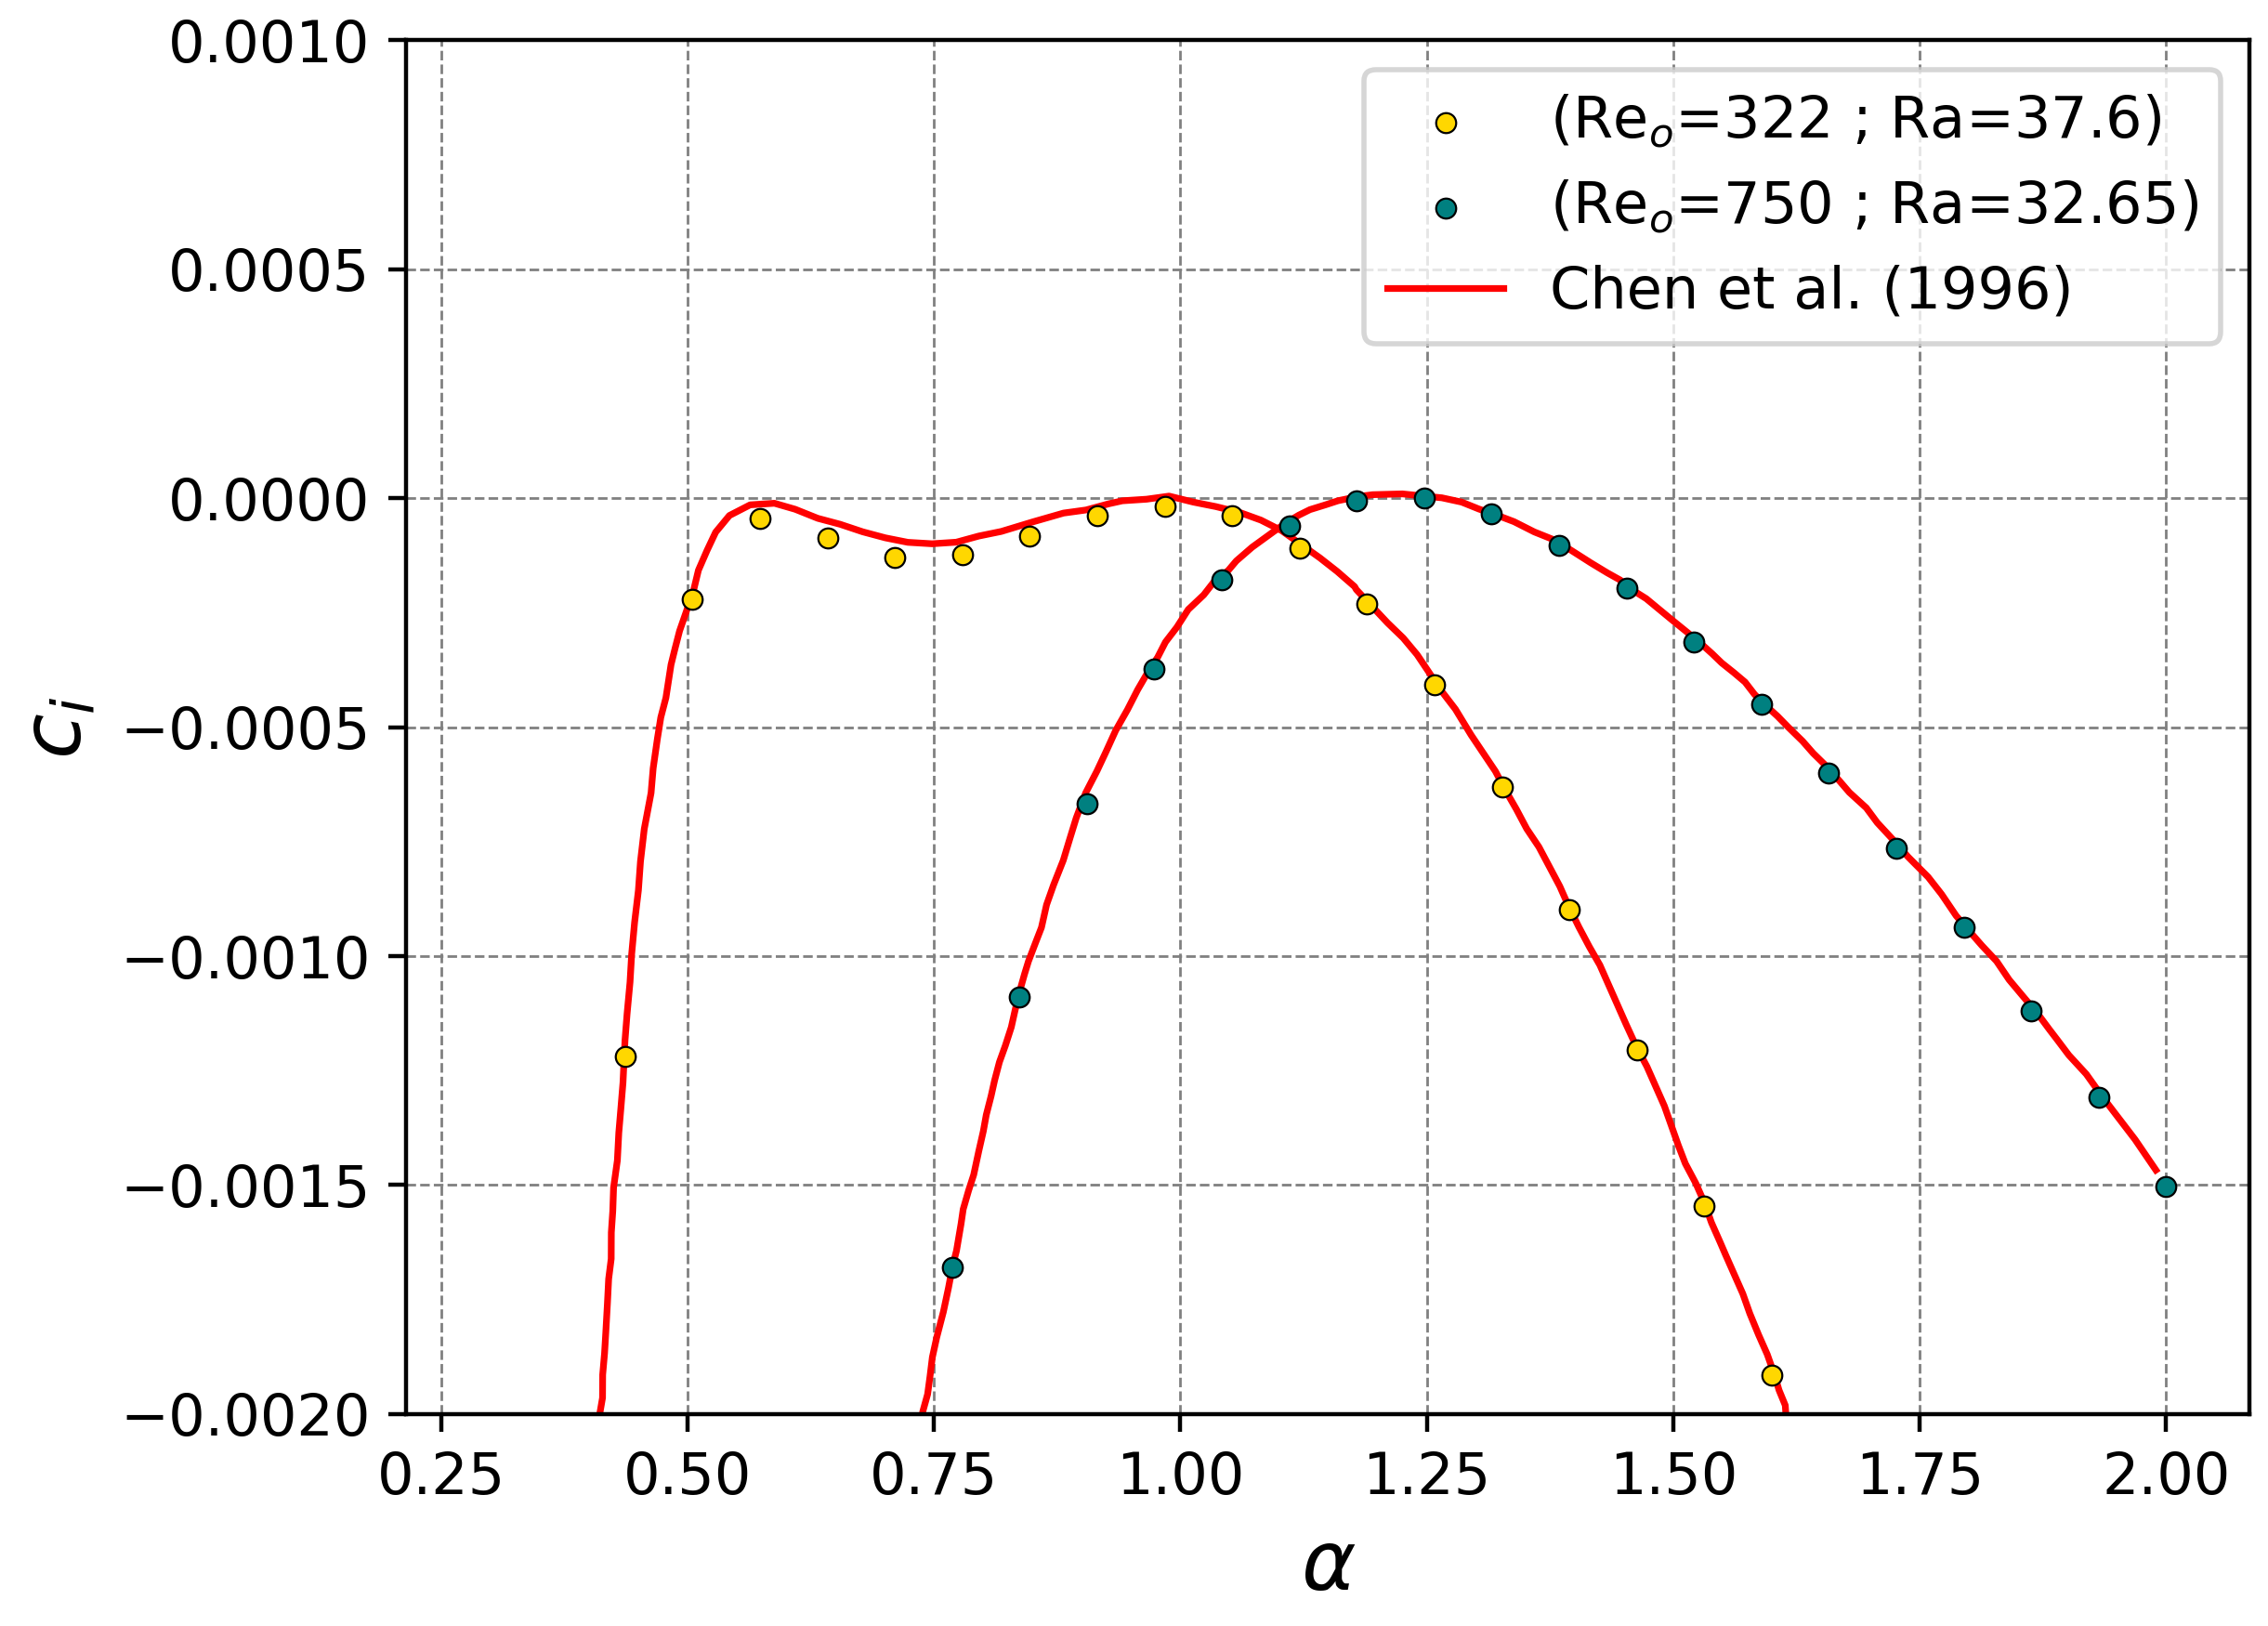
\includegraphics[width=0.6\textwidth]{figures/cap4/osmc/eigenvalues.png}
	 \caption{Variación de $c_i$ con $\alpha$ para diferentes valores de Re$_o$, a sus respectivos Ra.} 
 \label{fig:eigenval_alpha}
\end{figure}


\subsection{Autofunciones}

\paragraph{Normalización.}
Las autofunciones $\left\lbrace \widehat{v_x}(y),\widehat{v_y}(y),\widehat{v_z}(y), \widehat{\theta}(y) \right\rbrace_n$ se normalizan localizando el valor $y_i$ donde la norma de la autofunción $\widehat{v_x}$ es máxima, esto es: $\lVert \widehat{v_x} (y_i) \rVert = \max_{y} \lVert \widehat{v_x}(y) \rVert$; luego se elige un factor $c\in\mathbb{C}$ tal que $\operatorname{Re}\!\big[c\,\widehat{v_x}(y_i)\big]=1$ y $\operatorname{Im}\!\big[c\,\widehat{v_x}(y_i)\big]=0$. Con ese mismo factor $c$ se escalan todas las autofunciones: $\boldsymbol{\widehat{v}}_{\mathrm{norm}}=c\,\boldsymbol{\widehat{v}}$ y $\widehat{\theta}_{\mathrm{norm}}=c\,\widehat{\theta}$.

En la Figura \ref{fig:eigenfun_valid} se presentan las autofunciones correspondientes al autovalor más inestable asociado a los parámetros $\text{Re}_o=1125$, $\text{Ra}=2500$ y Pr = 0.7. La Figura \ref{fig:eigenfun_2d} expone la autofunción de la velocidad \textit{streamwise} y de la temperatura para el caso de una onda 2D al considerar $\alpha=1$ y $\beta=0$. Por su parte, la Figura \ref{fig:eigenfun_3d} presenta las autofunciones de las mismas magnitudes para una onda 3D ahora considerando $\alpha=1$ y $\beta=1$. Ambos casos se comparan con las autofunciones calculadas por Chen y Chung \cite{chen2003direct}. Aquí, los autores emplean una normalización distinta: cada una de las autofunciones $\left\lbrace \widehat{v_x}(y), \widehat{v_y}(y), \widehat{v_z}(y), \widehat{\theta}(y) \right\rbrace$ se normalizan de modo que el máximo de la parte real sea igual a uno y su fase sea nula. Al considerar esto y comparar las autofunciones obtenidas a partir OSMC, con aquellos obtenidos por Chen y Chung, es posible apreciar un excelente acuerdo.

\begin{figure}[H]
 \centering
  \subfloat[]{
    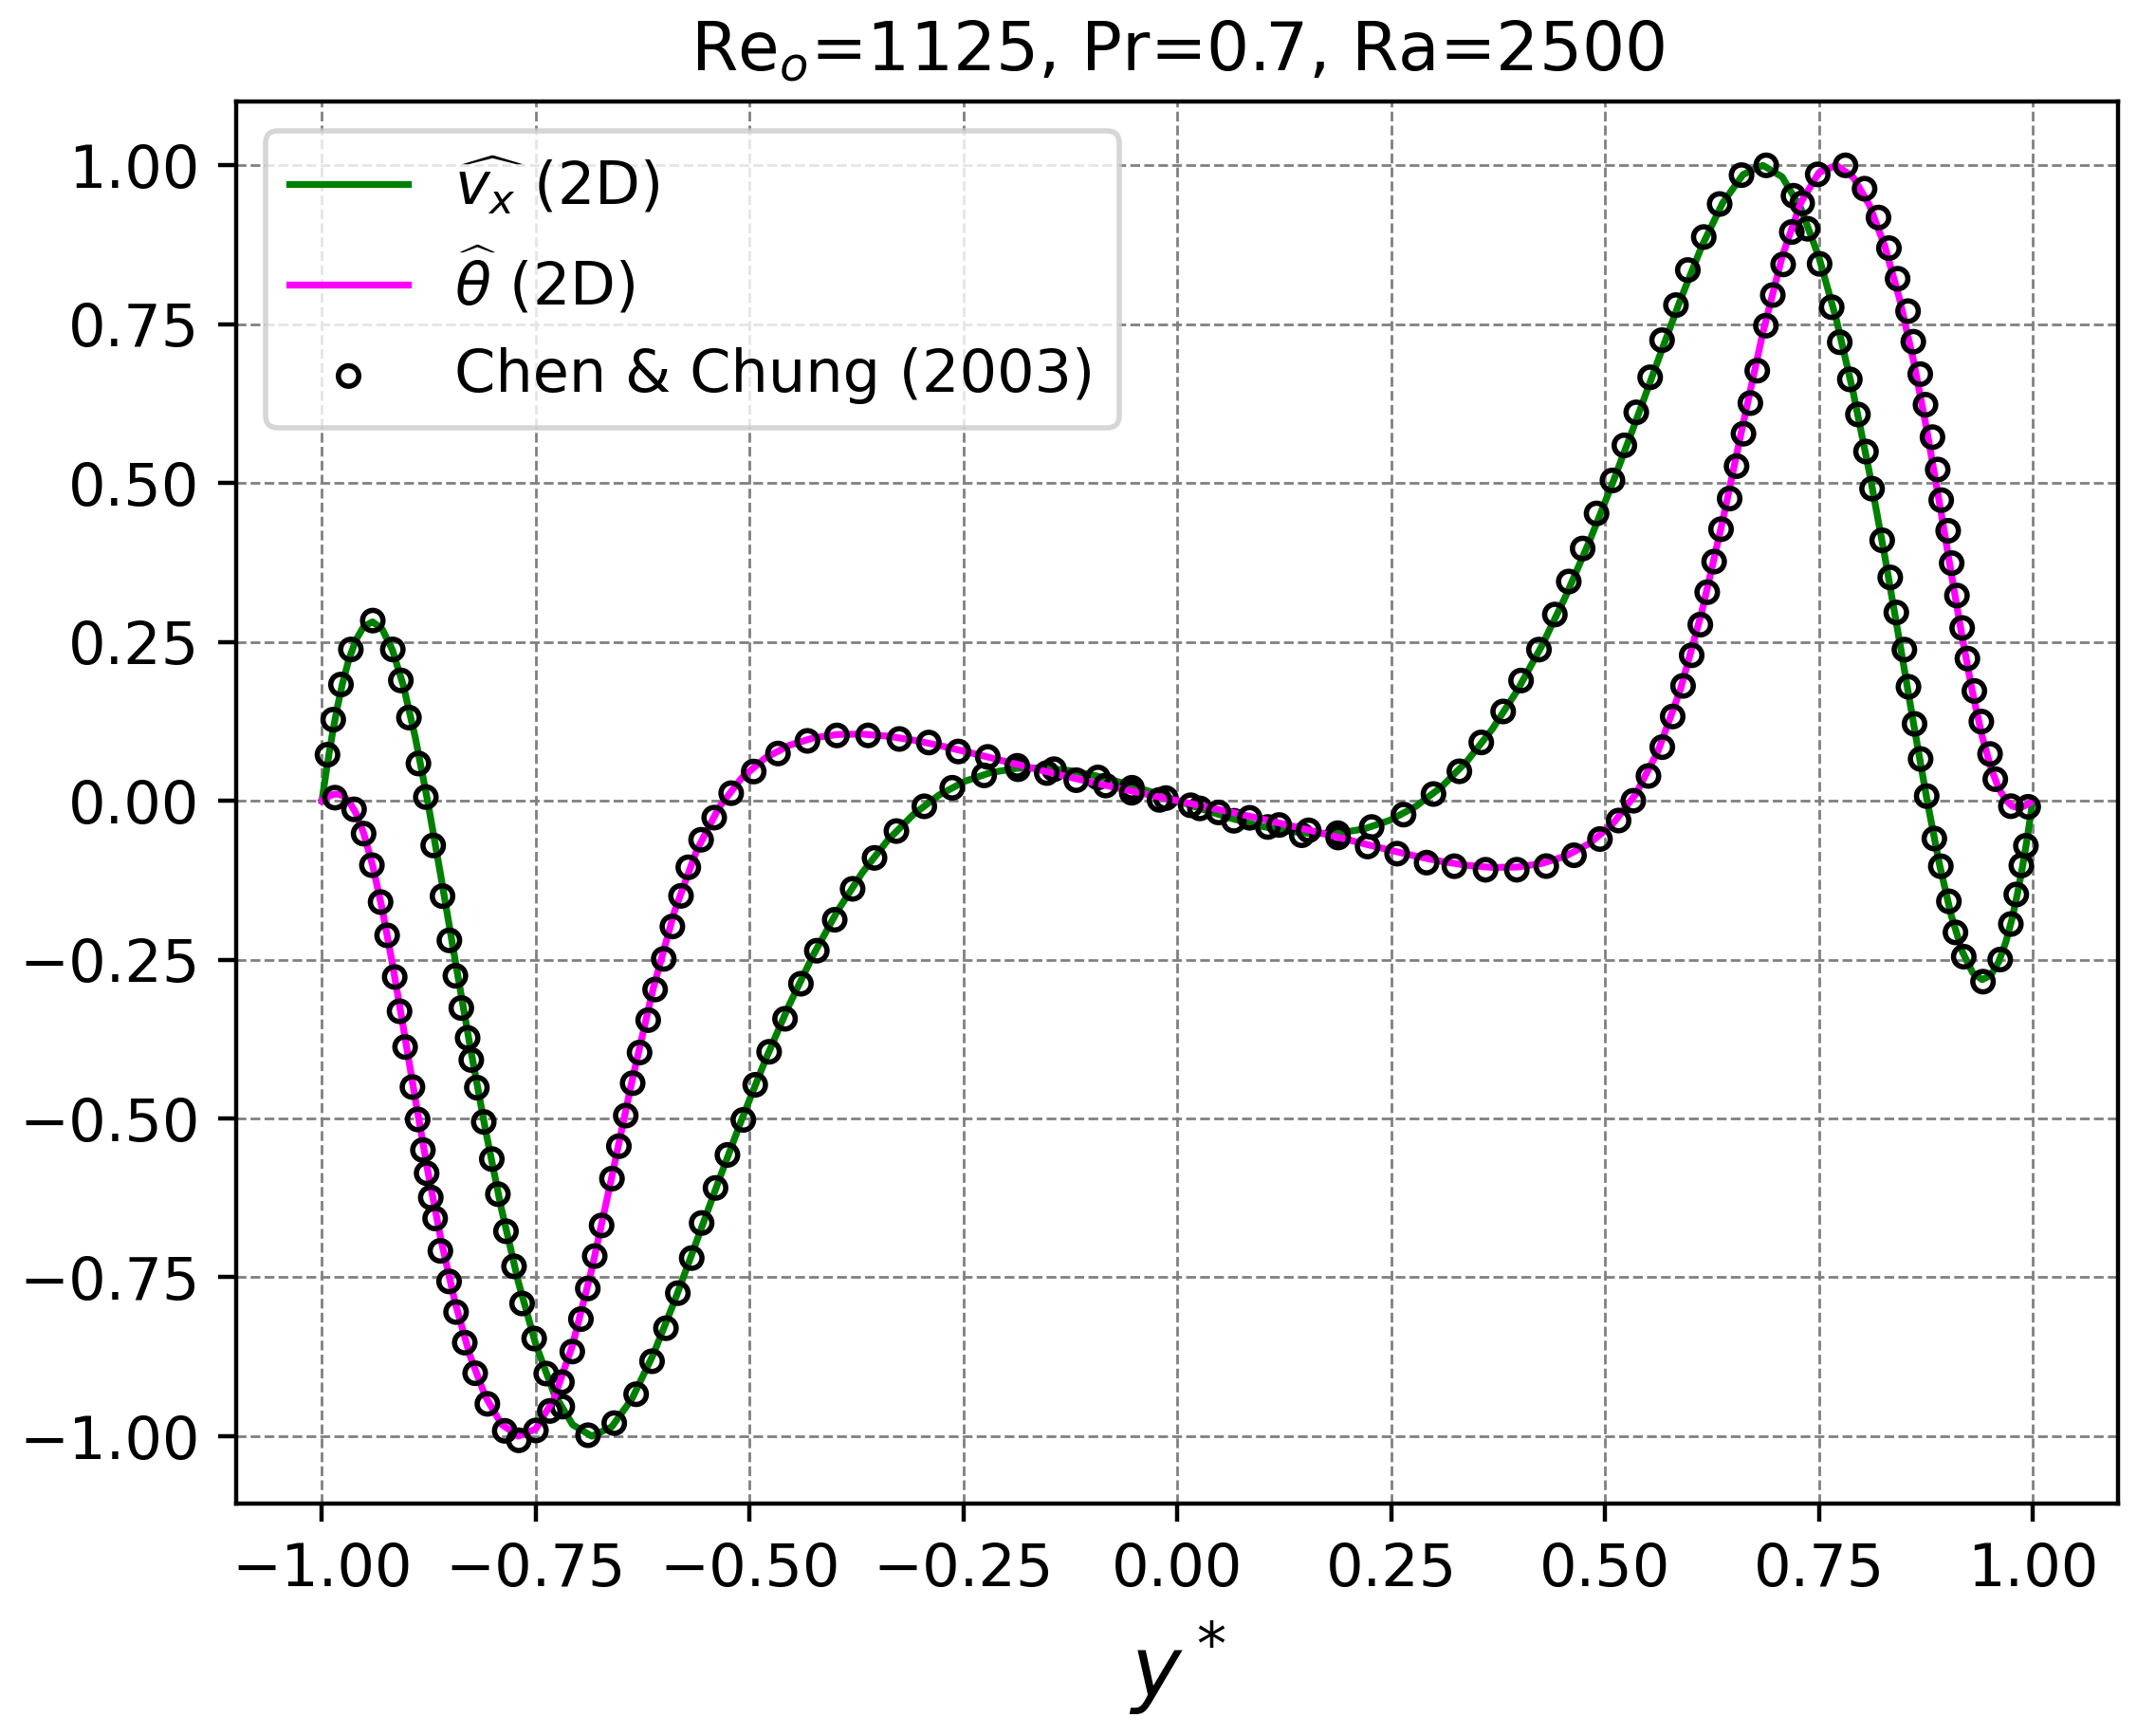
\includegraphics[width=0.49\textwidth]{figures/cap4/osmc/validation_eigenfuncs_2d.png}
    	\label{fig:eigenfun_2d}}  
    \subfloat[]{
    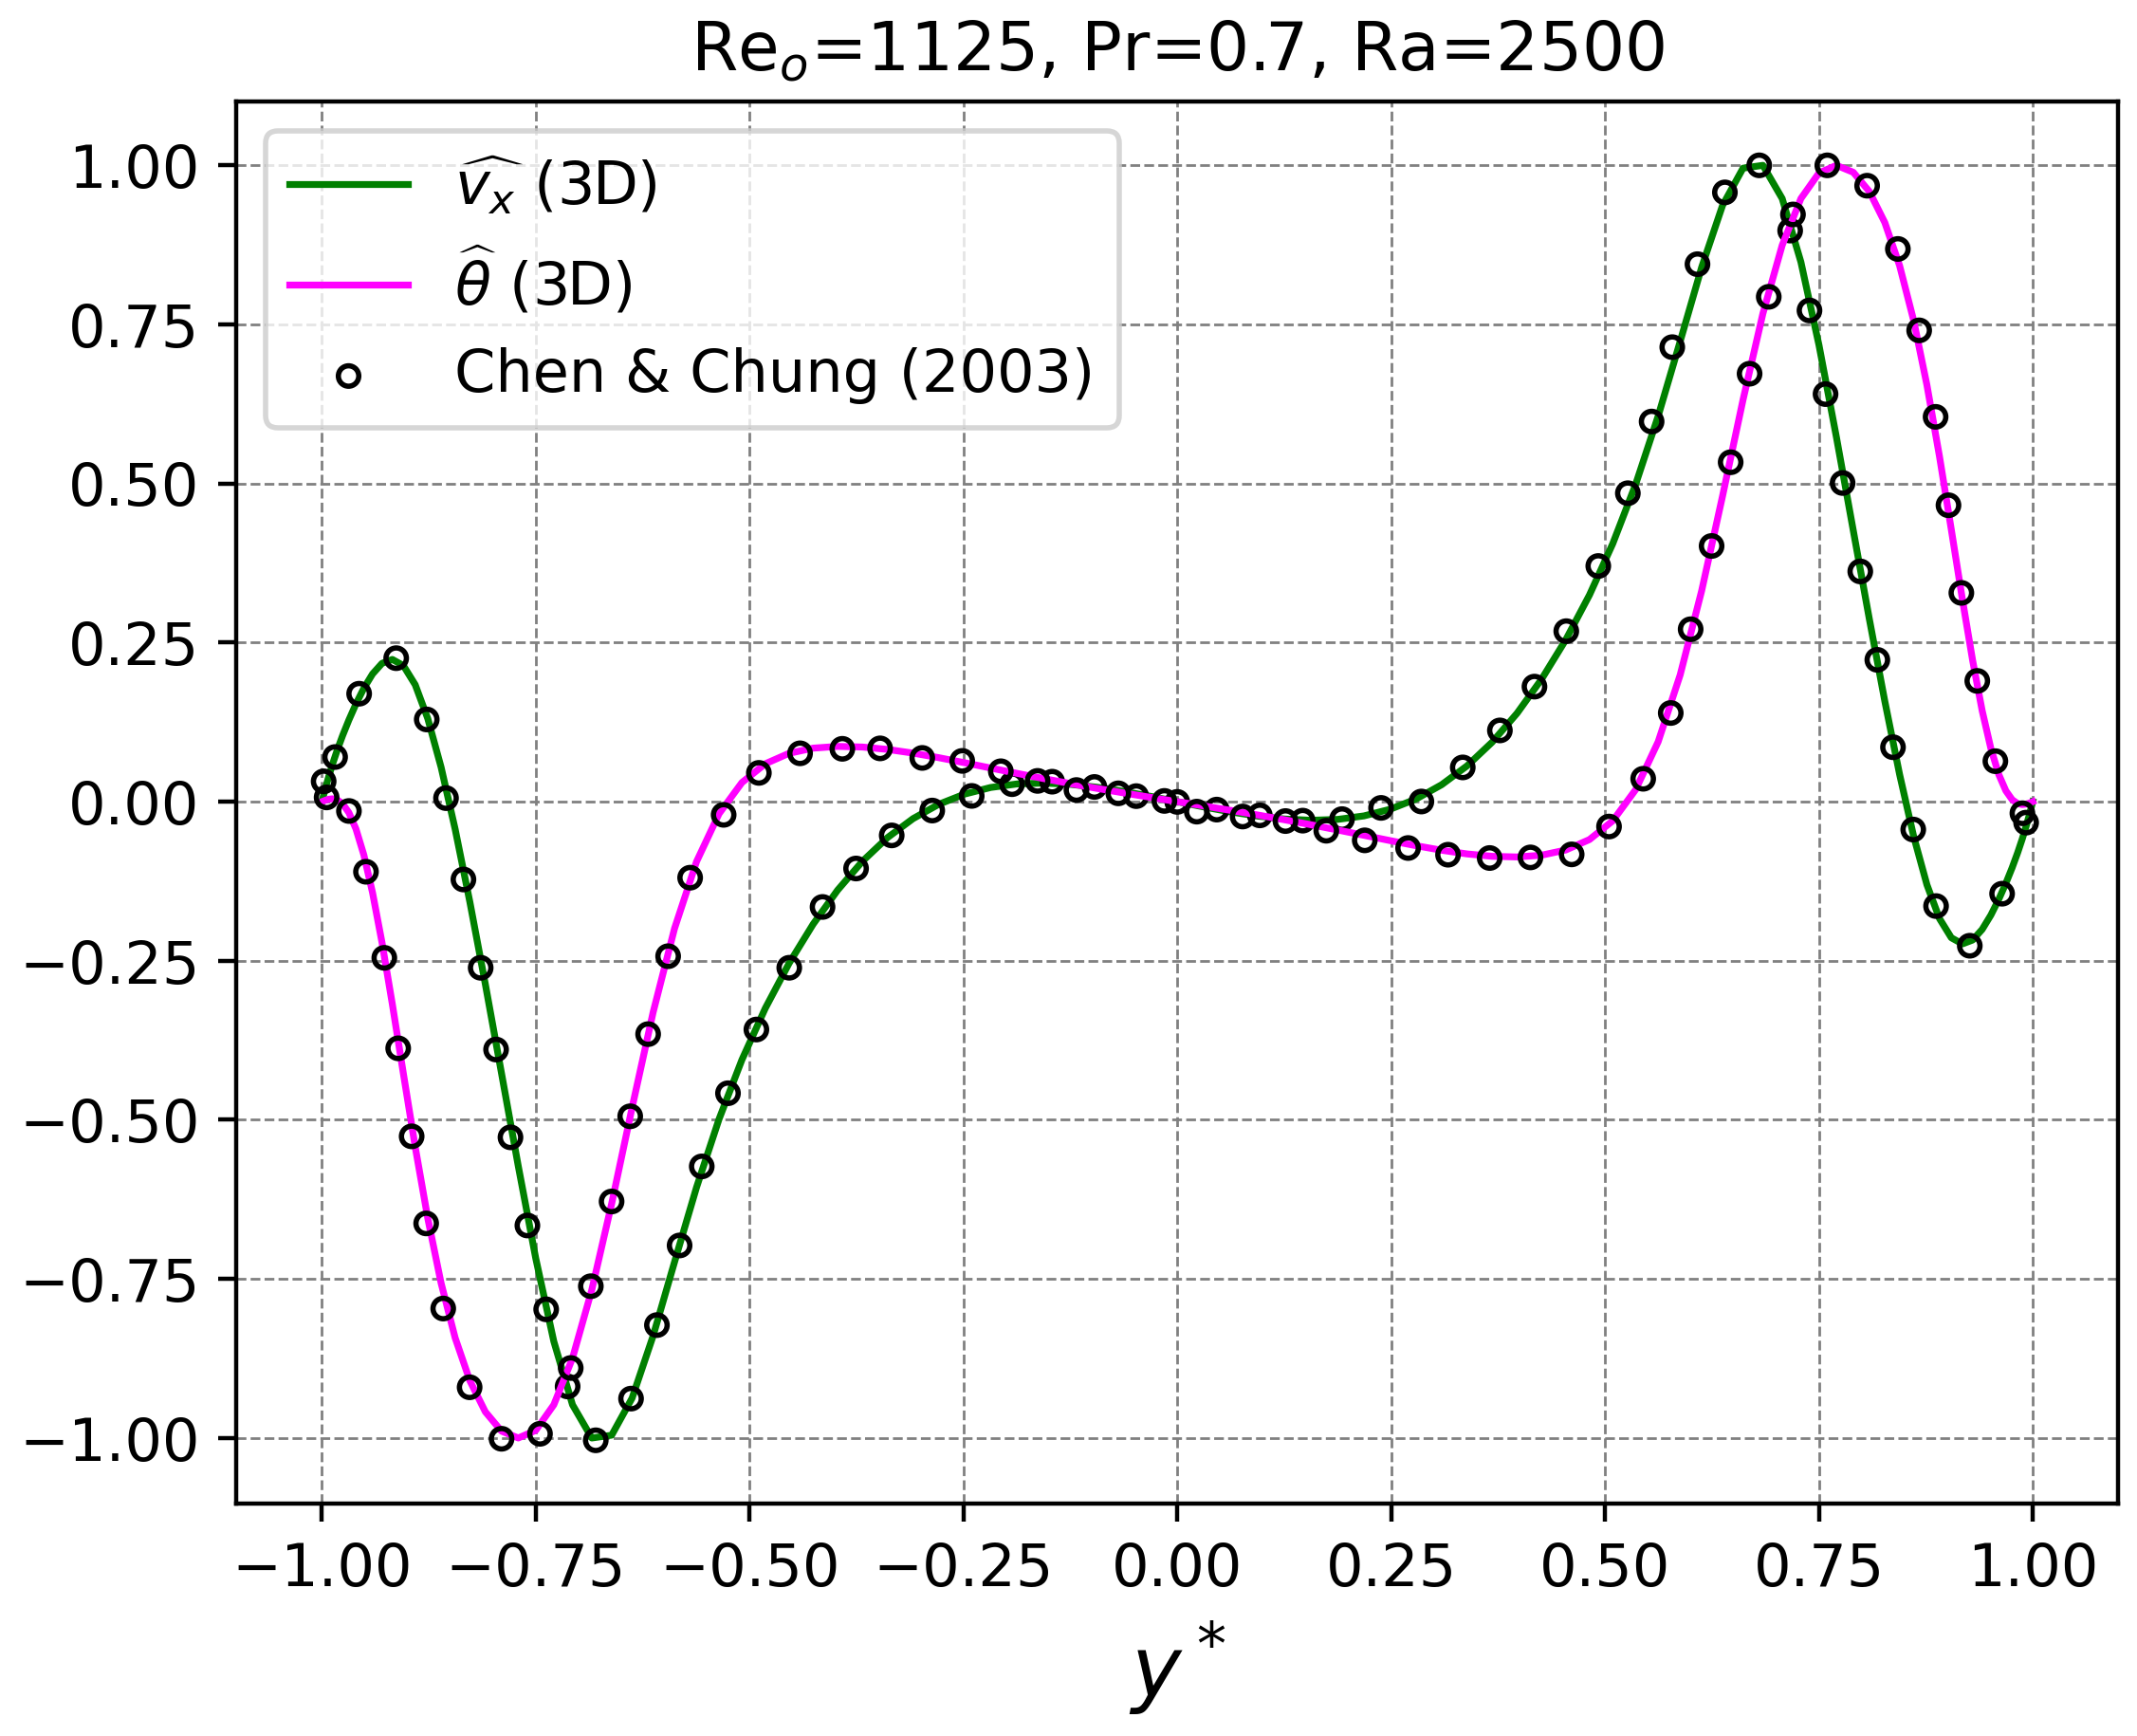
\includegraphics[width=0.49\textwidth]{figures/cap4/osmc/validation_eigenfuncs_3d.png}
    	\label{fig:eigenfun_3d}}  
 	\caption{Parte real de las autofunciones asociadas al modo más inestable para $\text{Re}_o=1125$, $\text{Ra}=2500$ y Pr = 0.7; \textbf{(a)} Onda 2D con ($\alpha$,$\beta$) = (1,0) y \textbf{(b)} Onda 3D con ($\alpha$,$\beta$) = (1,1).} 
 \label{fig:eigenfun_valid}
\end{figure}

\subsection{Análisis de Estabilidad Lineal versus DNS}

El análisis de estabilidad lineal predice a través de un modelo matemático la evolución temporal de pequeñas perturbaciones que son impuestas al flujo base. En esta sub-sección se pretende comparar dichas predicciones con los resultados arrojados por simulaciones realizadas con XC3D en escalas de tiempo donde las perturbaciones se mantienenen relativamente acotadas. Las condiciones iniciales de la simulación se construyen como la suma del flujo laminar, ecuaciones \ref{eq:vel_asist_boyant} - \ref{eq:theta_opo_boyant}, y las perturbaciones \ref{eq:init_con_1} - \ref{eq:init_con_3}. 

Se comparan dos casos, denominados RI y RD, cuyos números adimensionales corresponden a $\text{Re}_o=750$, Pr=0.7 y $\text{Ra}=65$. Los parámetros de simulación de ambos casos se exponen en la Tabla \ref{tab:caseslineal-theor}. Observese que se utilizan perturbaciones compuestas únicamente de ondas bidimensionales. El espectro de autovalores, junto con el autovalor seleccionado y sus autofunciones asociadas se muestran en la Figura \ref{fig:Ra65-2d}. Las simulaciones DNS realizadas se corren un total de 20 unidades temporales.

\begin{table}[H]
\centering
\resizebox{\textwidth}{!}{%
\begin{tabular}{lccccccccc}
\toprule
Caso & L$_x \times$ L$_y \times$ L$_z$ & N$_x \times$ N$_y \times$ N$_z$ & $\Delta t^*$ & $\alpha$ & $\beta$ & A$_{2D}$ & A$_{3D}$ & $\lambda_{2D}$ \\
\midrule
RI & $2 \pi / \alpha \times 2 \times 2 \pi $ & $160 \times 161 \times 160$ & 0.001 & 1.22 & 0 & 0.2 \% & 0 \% & 0.656 - 0.0237 j \\
RD & $2 \pi / \alpha \times 2 \times 2 \pi $ & $160 \times 161 \times 160$ & 0.001 & 1.22 & 0 & 0.2 \% & 0 \% & 1.239 + 0.042 j \\
\bottomrule
\end{tabular}}
\caption{Parámetros de simulación de los dos casos elegidos.}
\label{tab:caseslineal-theor}
\end{table}

Para comprobar la predicción de la teoría de estabilidad lineal con aquella producida por las herramientas numéricas, se emplea la evolución temporal de la energía cinética turbulenta (TKE) y de la varianza de la temperatura. En XC3D, dichas magnitudes corresponden al promedio integral en $y^*$ de las correlaciones $( \langle u^{* \prime}_x u^{* \prime}_x \rangle + \langle u^{* \prime}_y u^{* \prime}_y  \rangle + \langle u^{* \prime}_z u^{* \prime}_z  \rangle) / 2$ y $\langle \theta^{* \prime} \theta^{* \prime} \rangle$, mientras que para teoría de estabilidad lineal dichas cantidades se aproximan utilizando las autofunciones $\left\lbrace \widehat{v_x}, \widehat{v_y}, \widehat{v_z}, \widehat{\theta} \right\rbrace$ y las expresiones tipo \ref{eq:waves3d} para obtener:
\begin{align}
\text{TKE} &\simeq \frac{1}{2} (A_{2D})^2 \hspace*{0.5mm} e^{2 \alpha c_i t^*} \int \left[  ( \widehat{v_x}, \widehat{v_y}, \widehat{v_z} ) \cdot ( \widehat{v_x}, \widehat{v_y}, \widehat{v_z} )  \right] dy^* \\
\int \langle \theta^{* \prime} \theta^{* \prime} \rangle dy^* &\simeq \frac{1}{2} (A_{2D})^2 \hspace*{0.5mm} e^{2 \alpha c_i t^*} \int (\widehat{\theta})^2 dy^*
\end{align}   
En estas expresiones, si $c_i < 0$, las cantidades decaen y el flujo es estable. Pero por el contrario, si $c_i > 0$, la mismas crecen y el flujo base evoluciona en el tiempo, dando posiblemente, origen a la transición. Las afirmaciones anteriores son ciertas siempre que $\alpha$ sea positivo.

En las Figuras \ref{fig:Ra65RD-tke} y \ref{fig:Ra65RD-tvar} muestran la evolución temporal de la TKE y de la varianza de la temperatura para el caso RD. Se observa un muy buen acuerdo entre la predicción teórica y los resultados obtenidos a partir de simulaciones DNS con las herramientas numéricas utilizadas. En este caso se aprecia que la perturbación introducida logra inestabilizar el flujo (pues $c_i>0$) y que si bien en una etapa temprana el acuerdo entre ambas metodologías coincide, si el flujo transiciona a un régimen turbulento, la consistencia entre ambos debería tender a desaparecer.  

De forma completamente análoga, las Figuras \ref{fig:Ra65RI-tke} y \ref{fig:Ra65RI-tvar} muestran la evolución temporal de la TKE y de la varianza de la temperatura para el caso RI. En este caso, dado que $c_i<0$, el análisis de estabilidad lineal predice que la perturbación impuesta tenderá a decaer y el flujo no se inestabilizará, esta predicción esta en completa consistencia con la simulación DNS realizada.   

\begin{figure}[H]
 \centering
  \subfloat[]{
    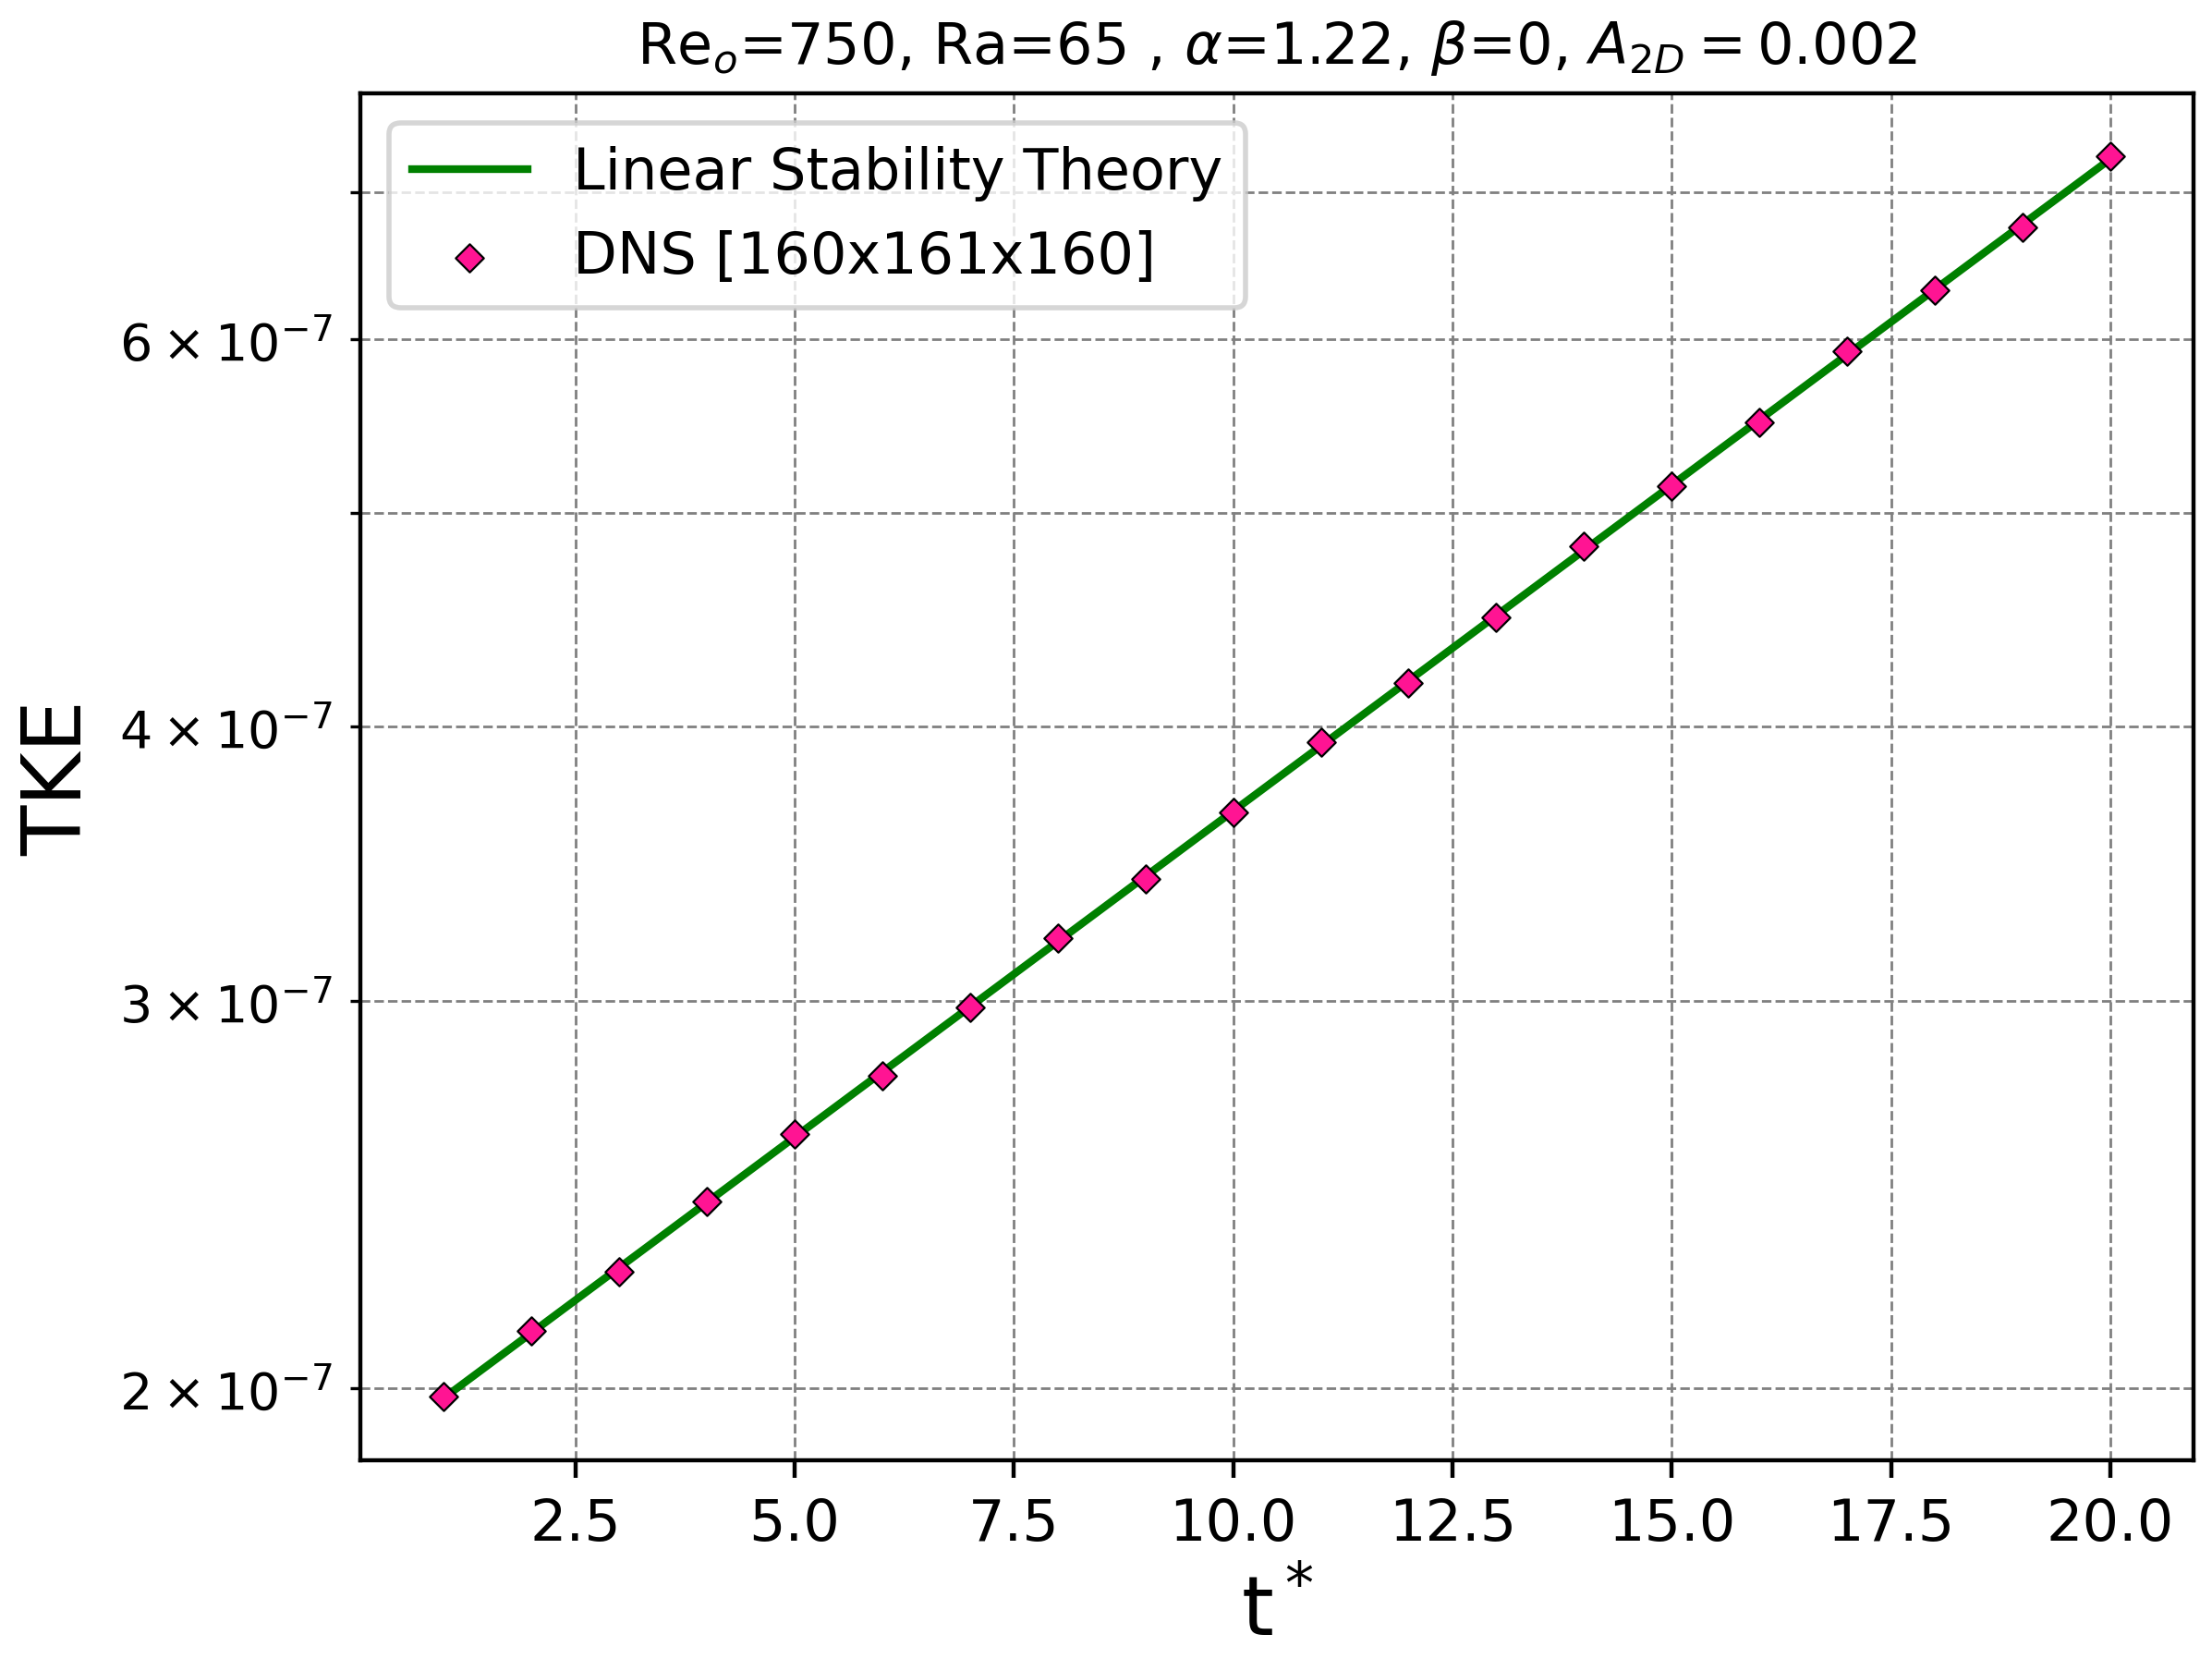
\includegraphics[width=0.49\textwidth]{figures/cap4/osmc/Ra65_RamaDer/tke.png}
    	\label{fig:Ra65RD-tke}}  
  \subfloat[]{
    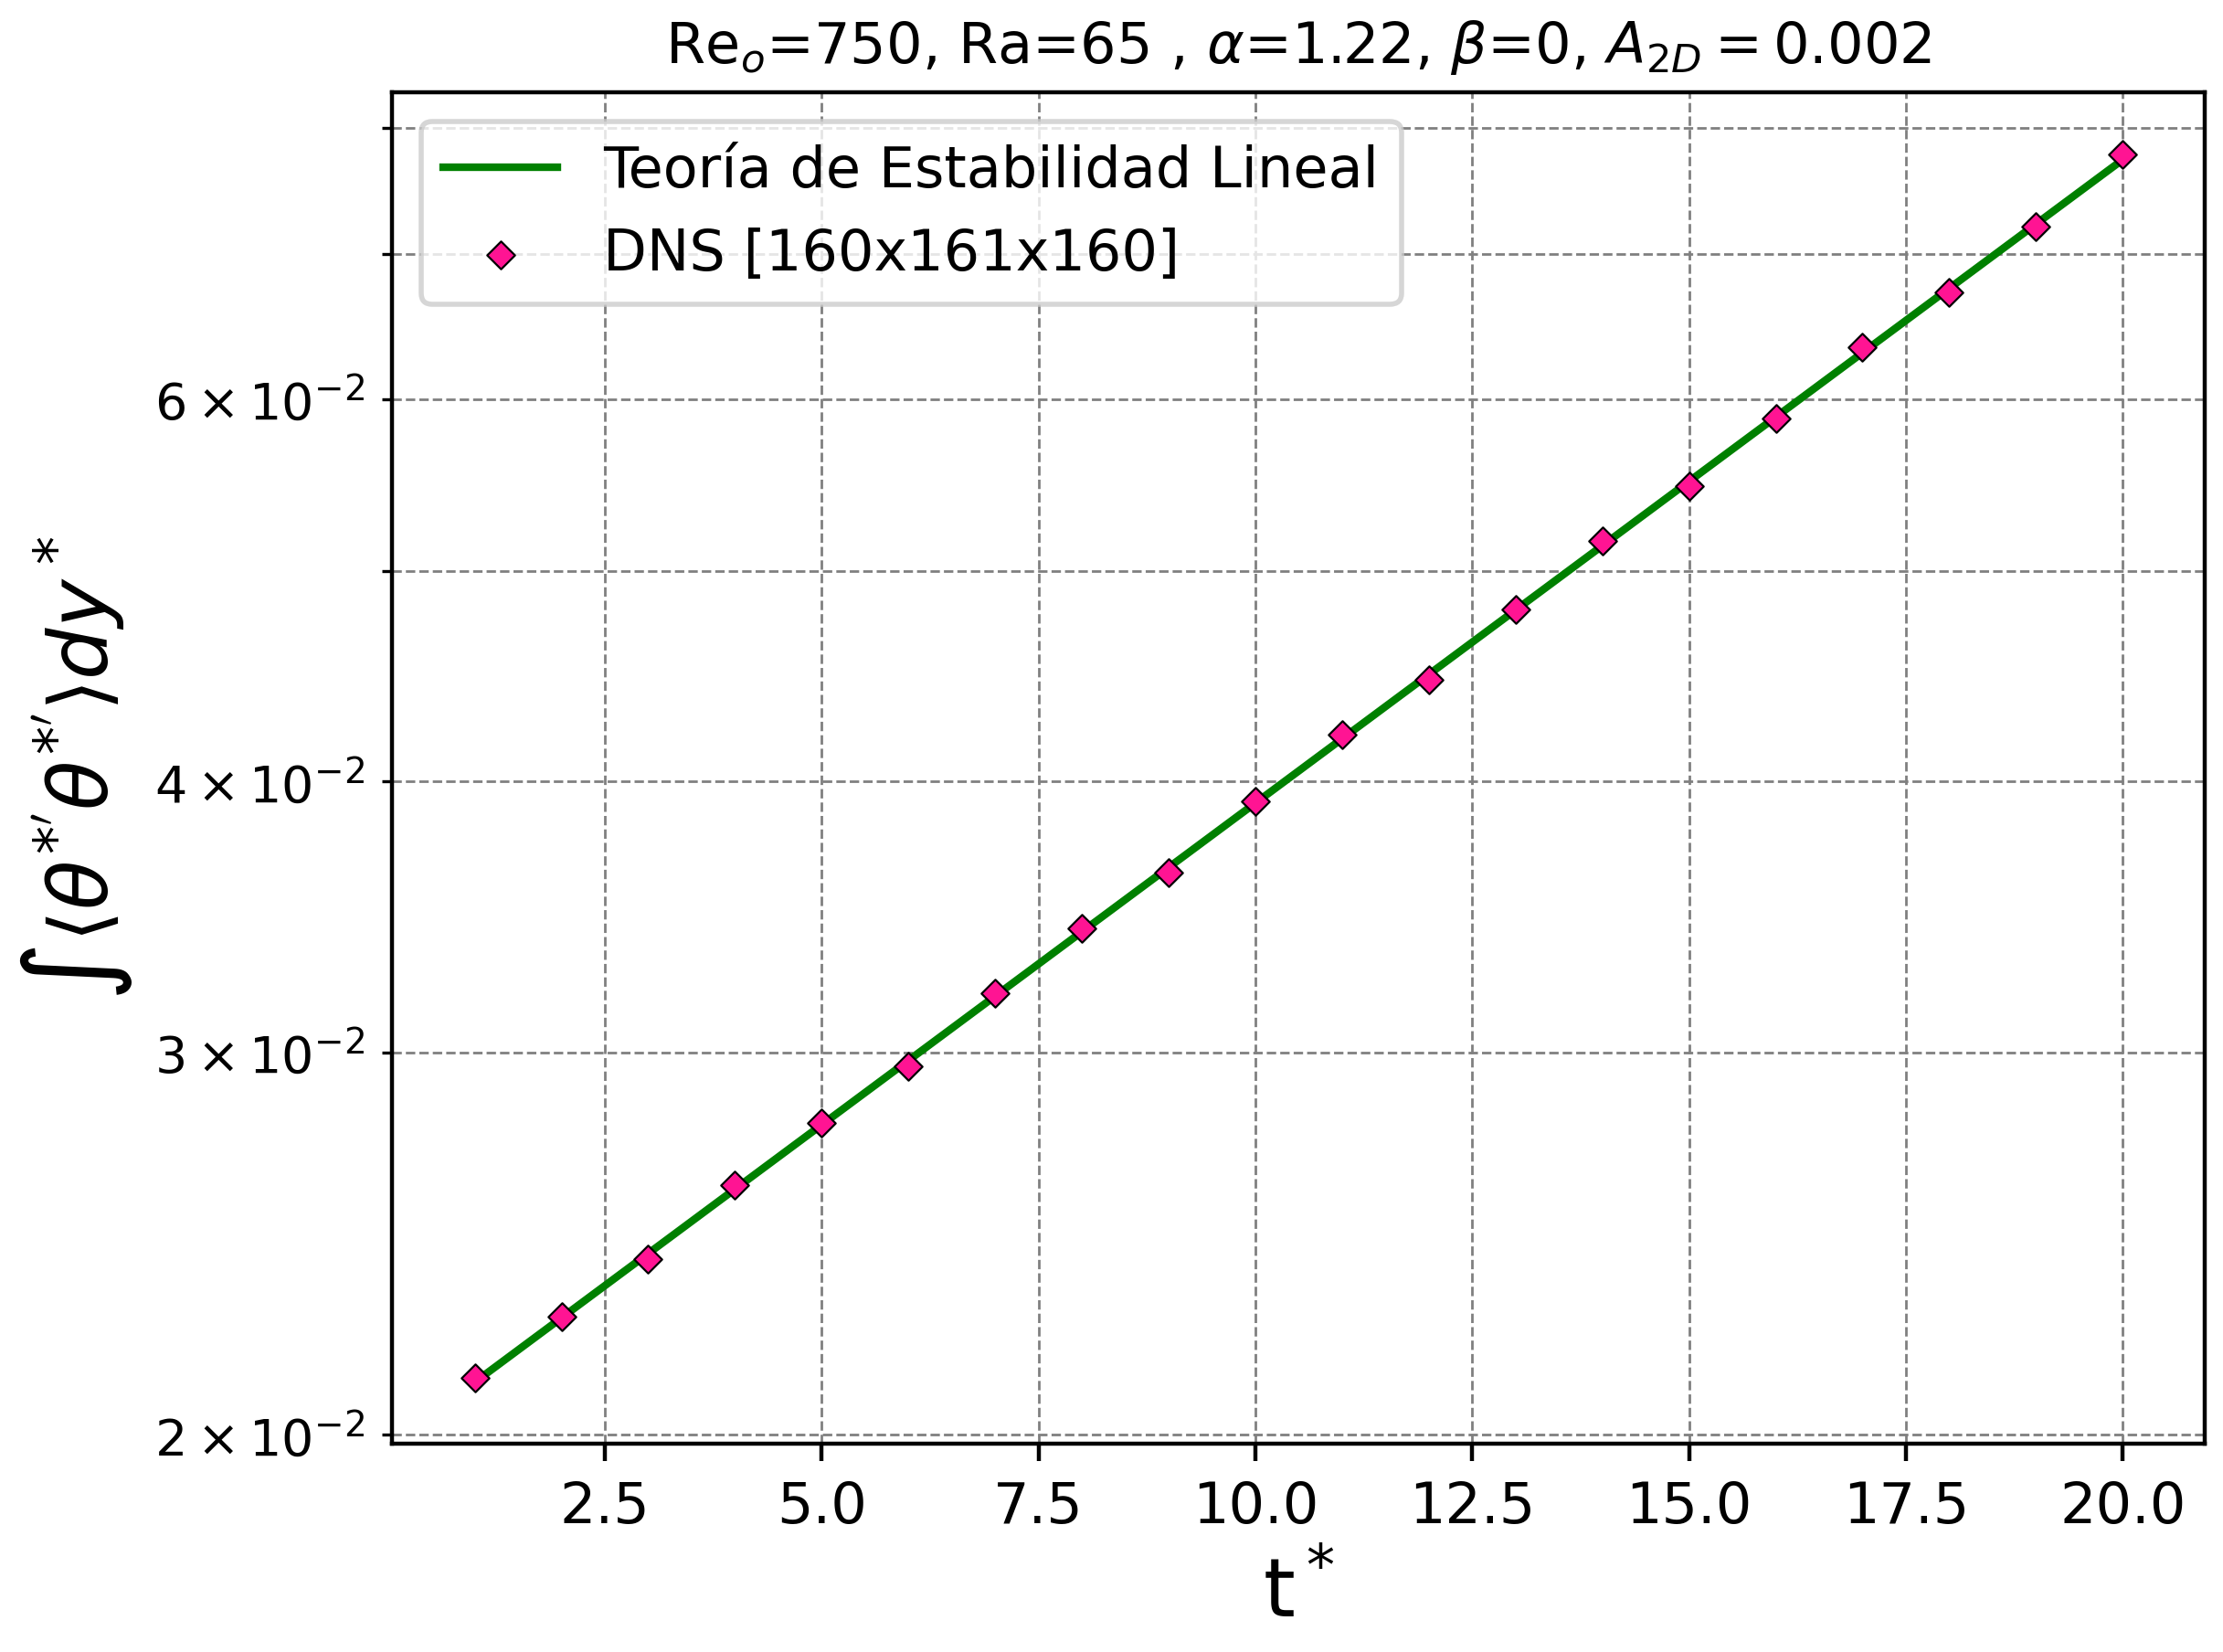
\includegraphics[width=0.49\textwidth]{figures/cap4/osmc/Ra65_RamaDer/theta_var.png}
    	 \label{fig:Ra65RD-tvar}}  
 \caption{Evolución temporal de la varianza de la temperatura y de la TKE del caso RD.} 
 \label{fig:Ra65R-DI}
\end{figure}

\begin{figure}[H]
 \centering
  \subfloat[]{
    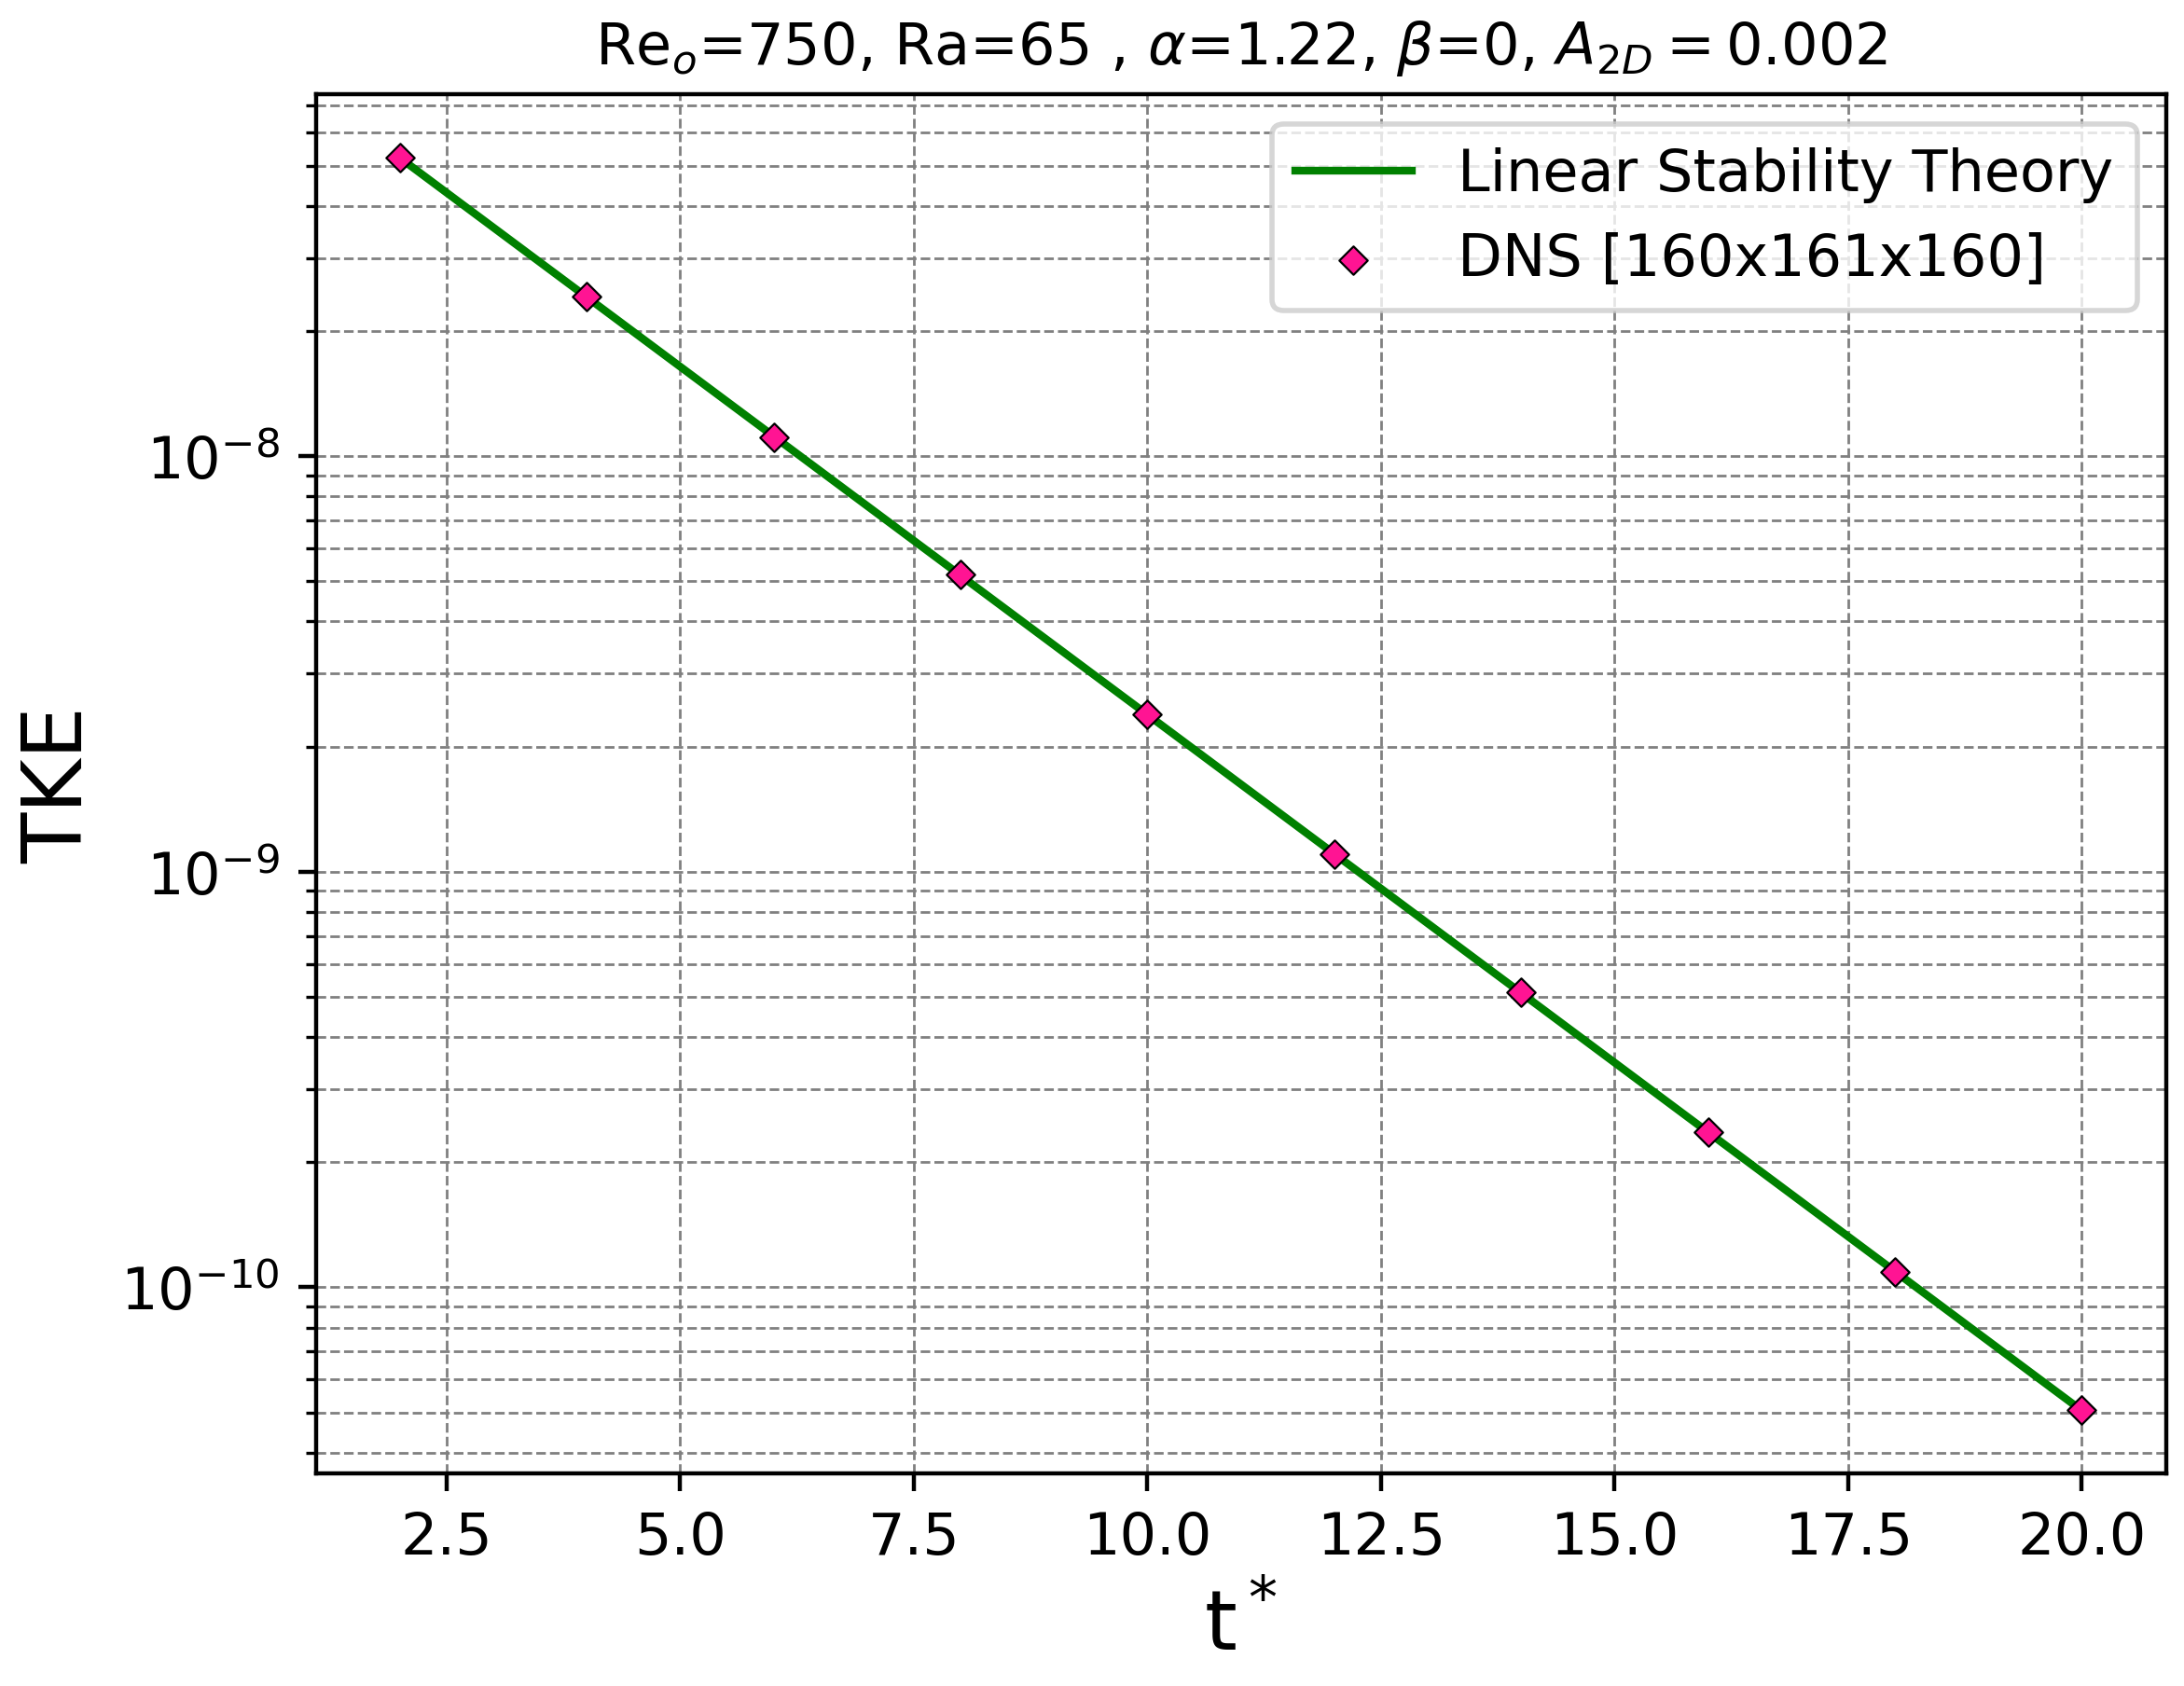
\includegraphics[width=0.49\textwidth]{figures/cap4/osmc/Ra65_RamaIzq/tke.png}
    	\label{fig:Ra65RI-tke}}  
  \subfloat[]{
    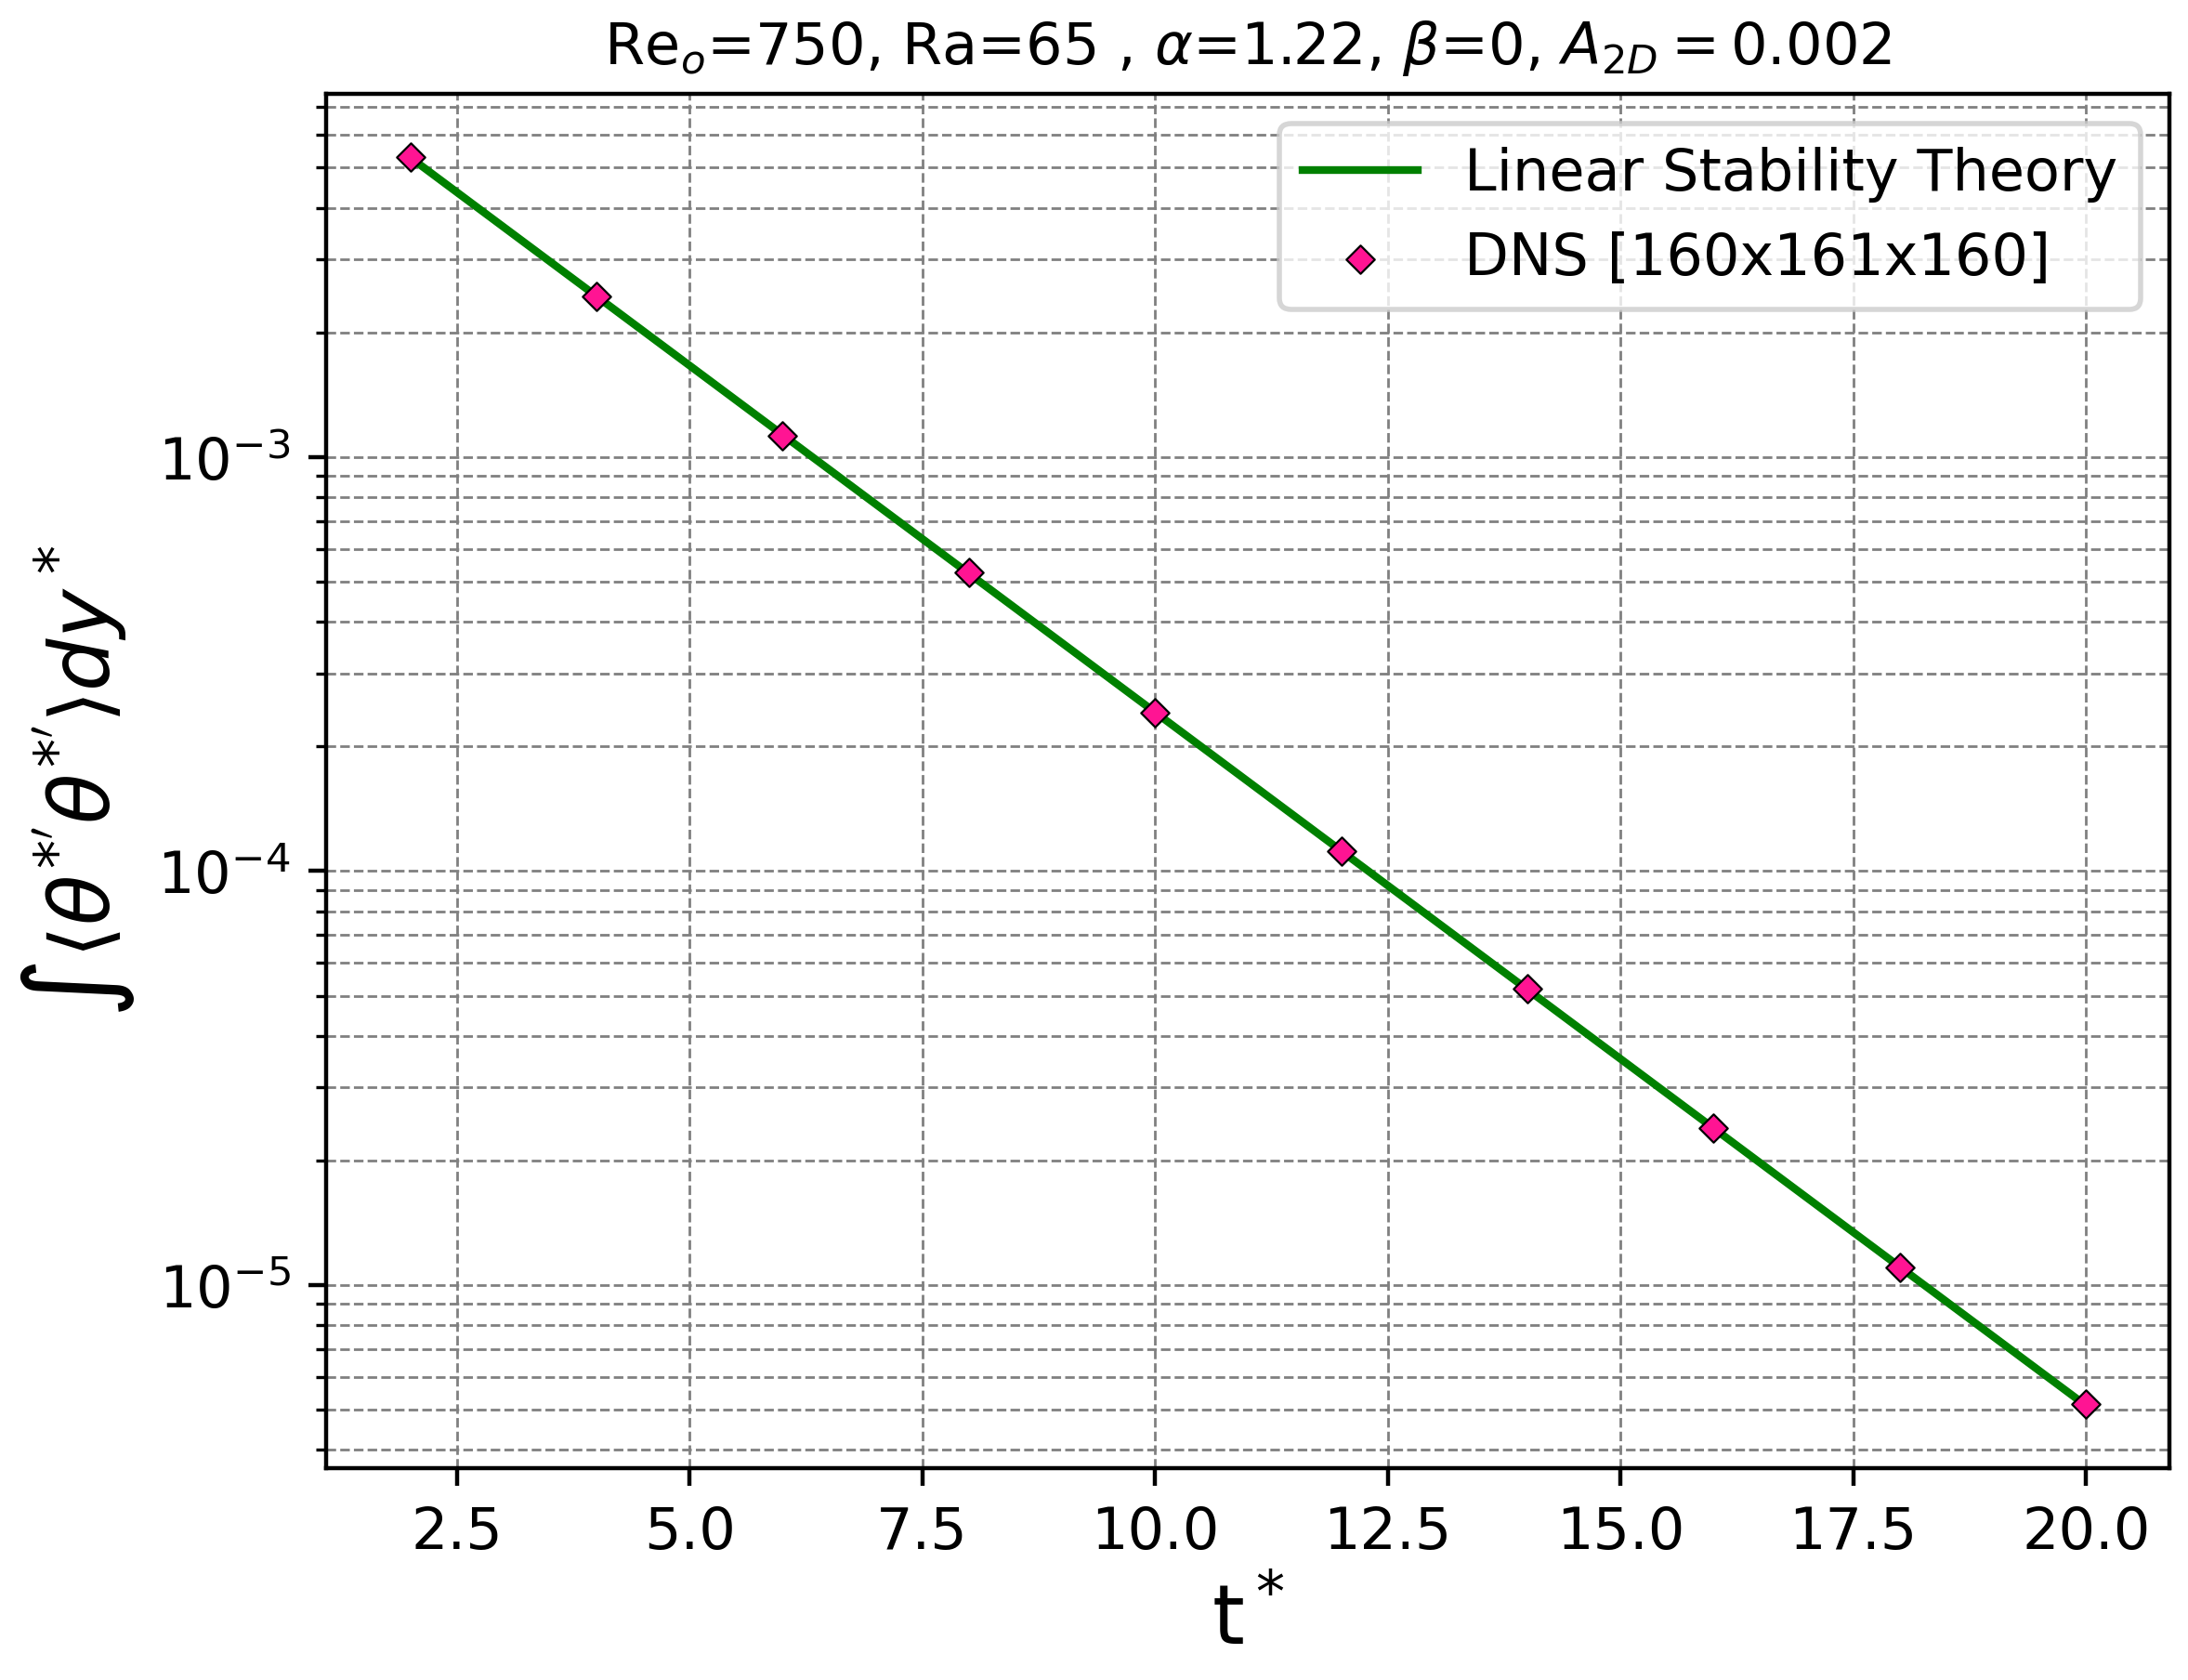
\includegraphics[width=0.49\textwidth]{figures/cap4/osmc/Ra65_RamaIzq/theta_var.png}
         \label{fig:Ra65RI-tvar}}  
 \caption{Evolución temporal de la varianza de la temperatura y de la TKE del caso RI.} 
 \label{fig:Ra65R-DI}
\end{figure}

\begin{figure}[H]
 \centering 
  \subfloat[]{
    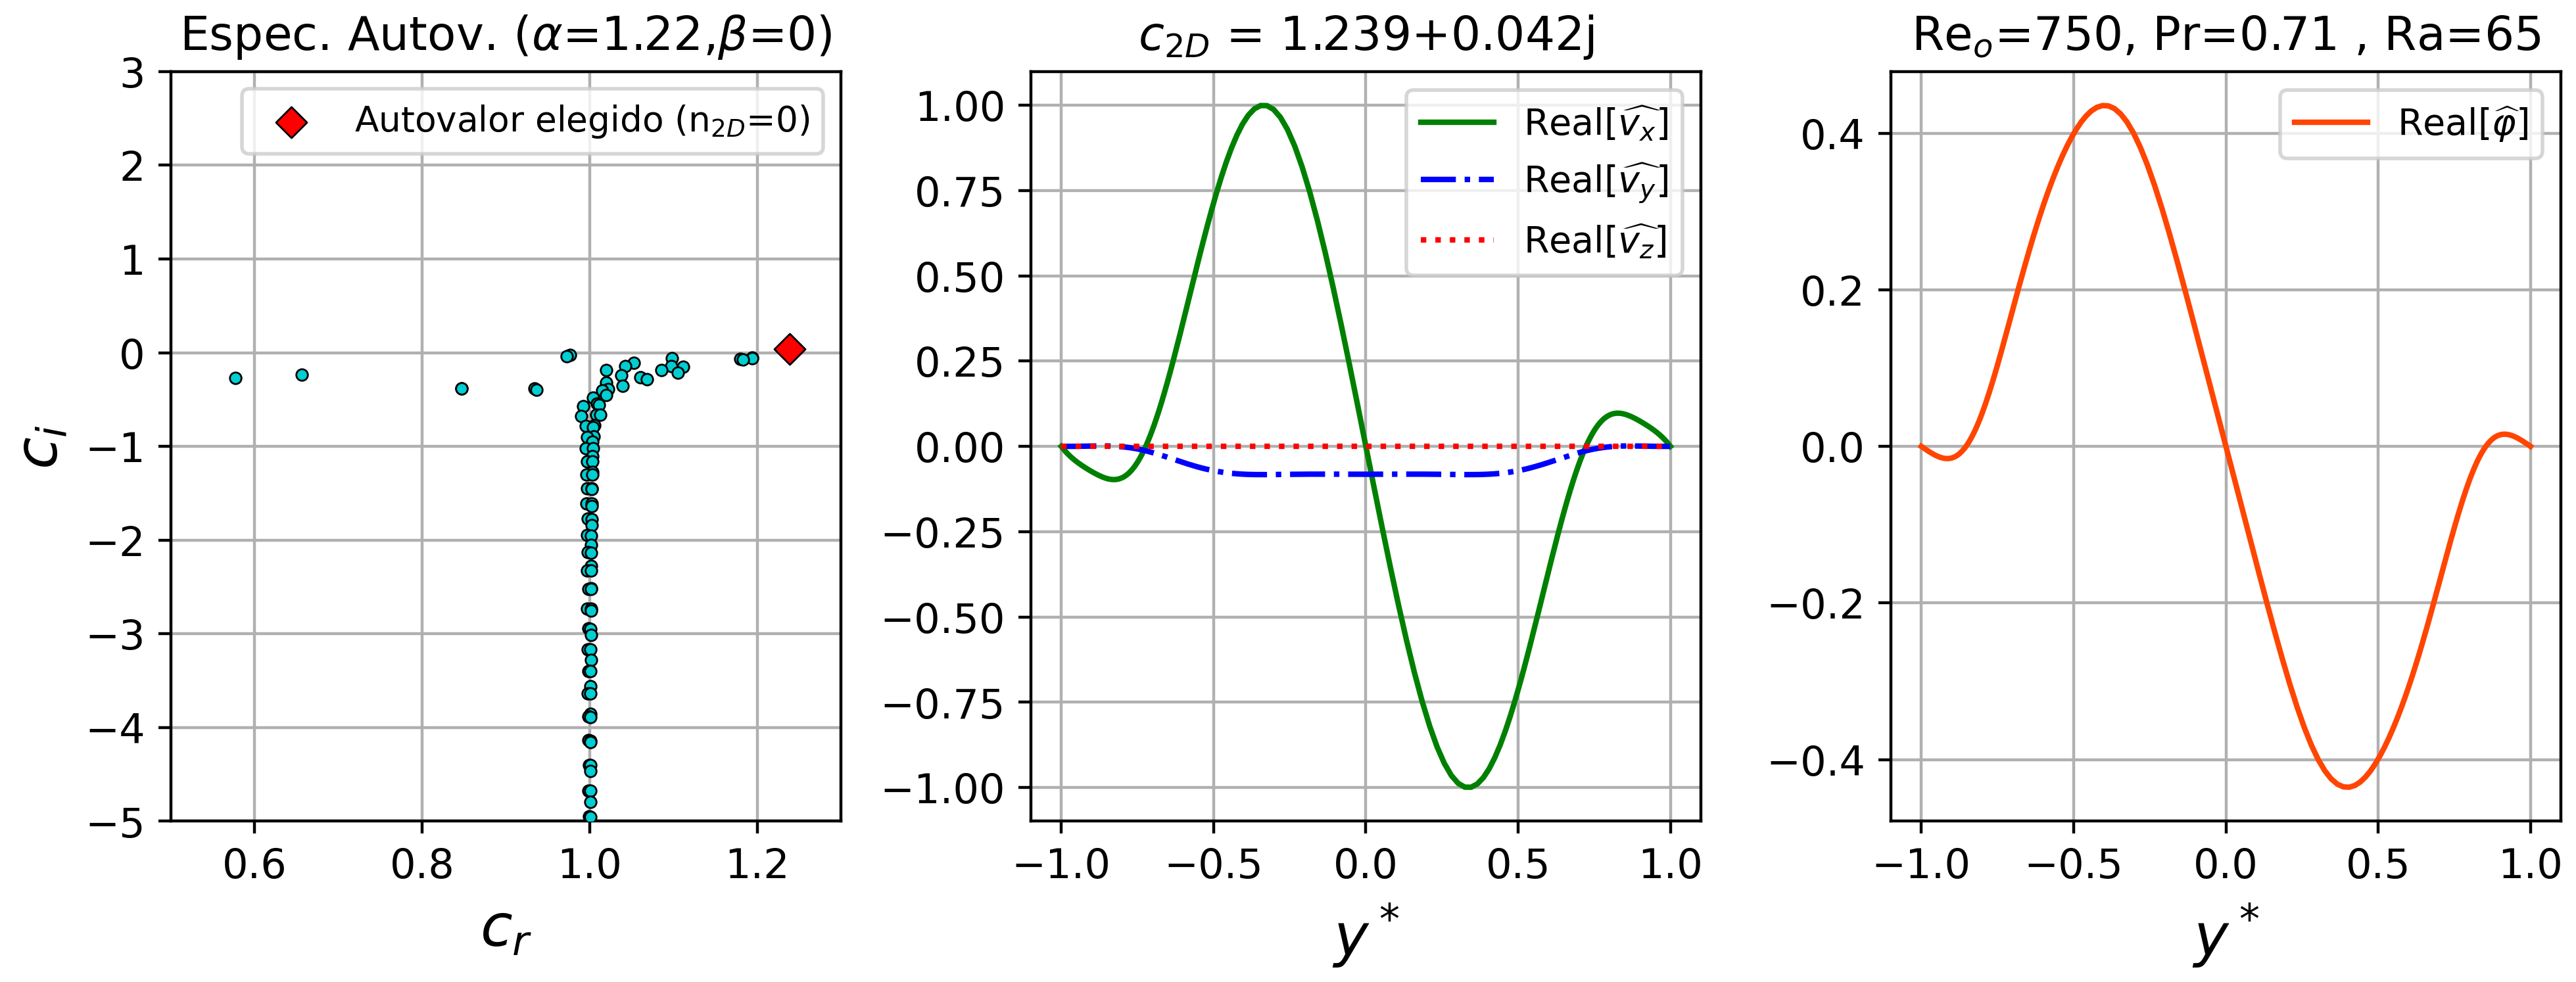
\includegraphics[width=0.8\textwidth]{figures/cap4/osmc/Ra65_RamaDer/2d_eigenfun.png}
    \label{fig:Ra65RD-2d}}
      
    \subfloat[]{
    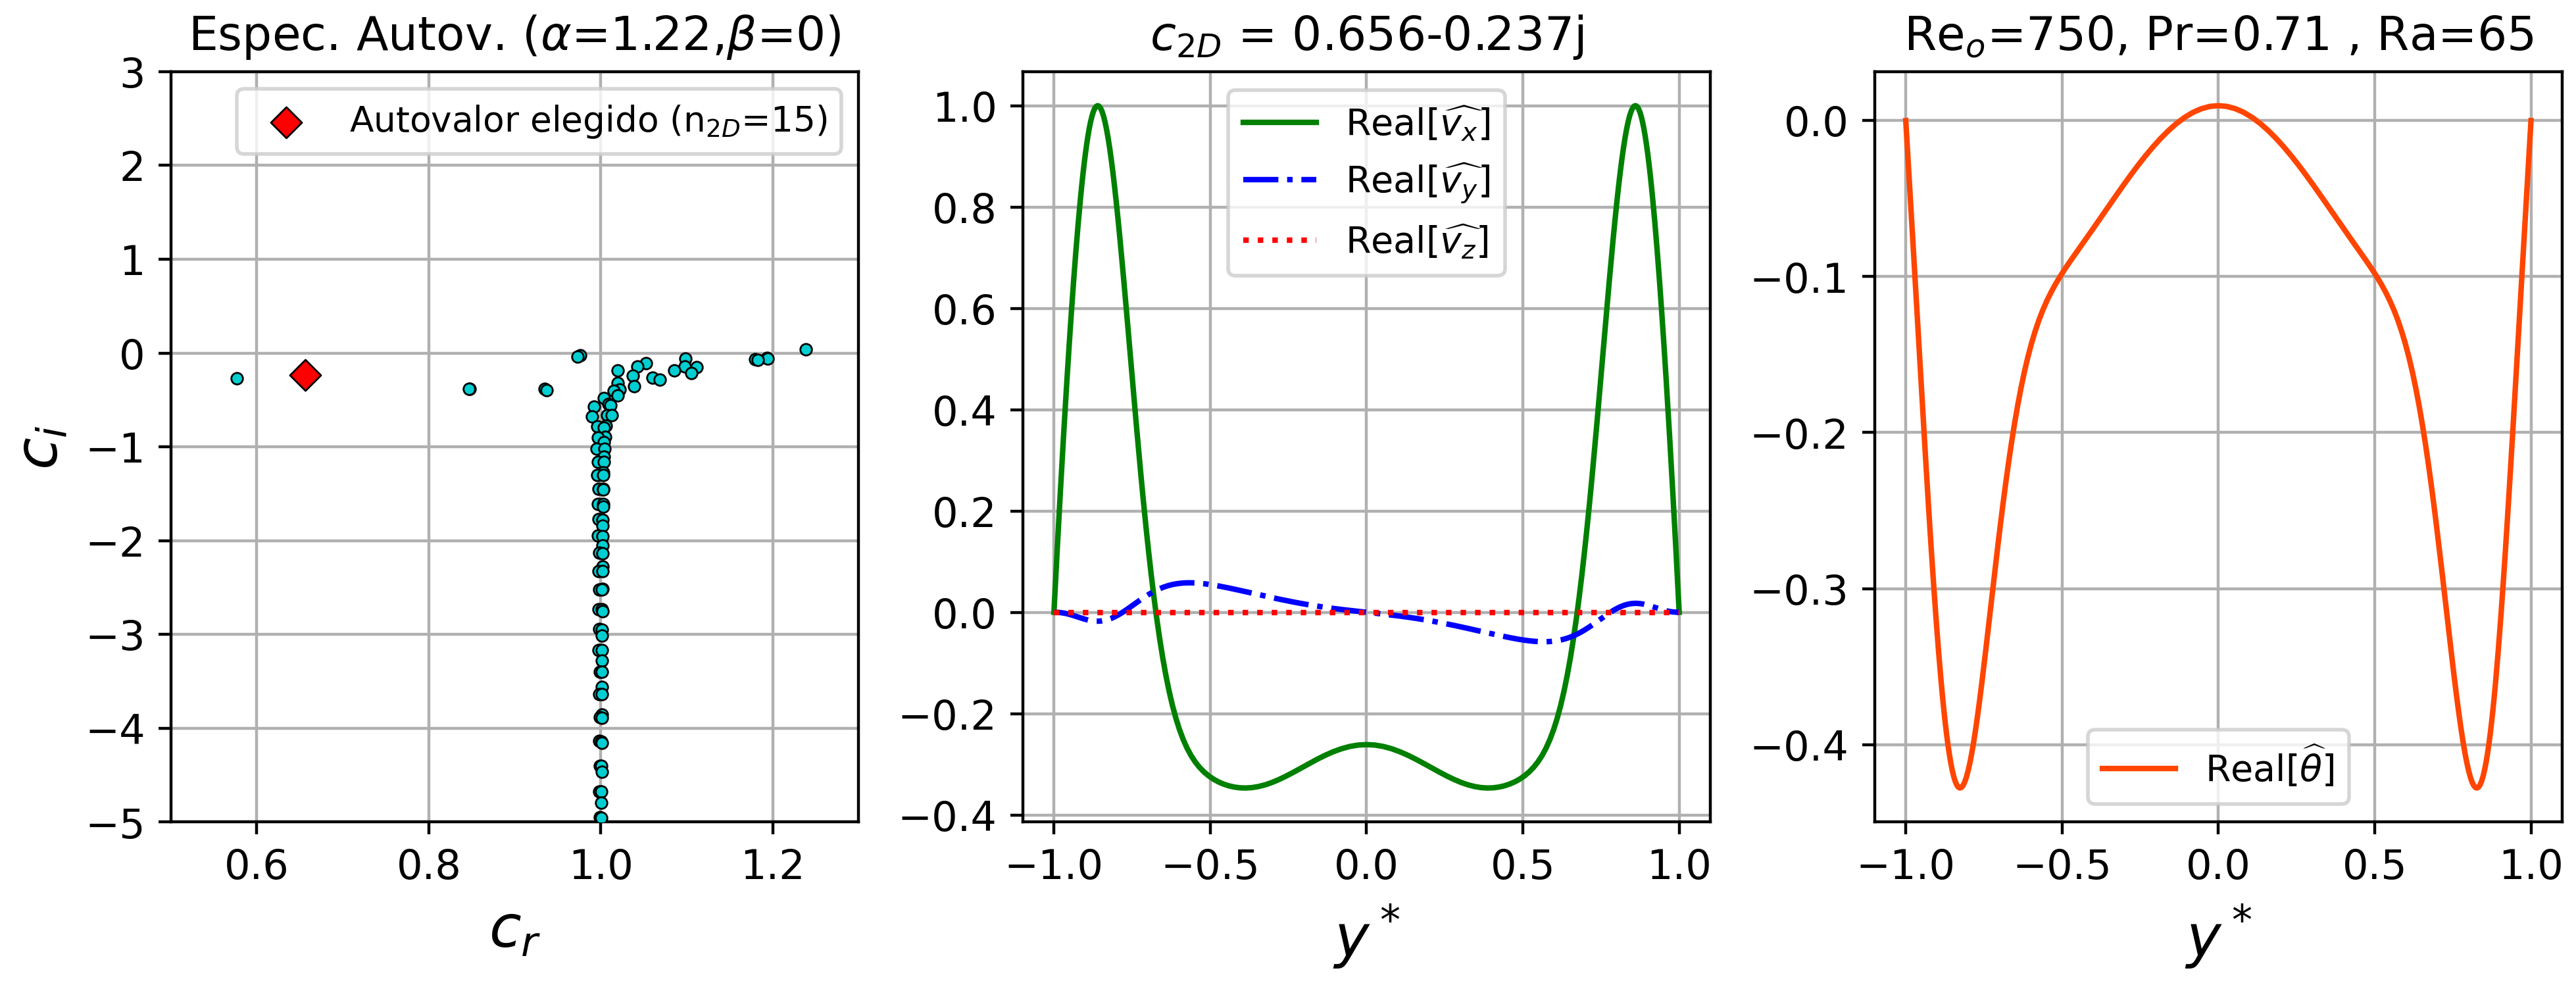
\includegraphics[width=0.8\textwidth]{figures/cap4/osmc/Ra65_RamaIzq/2d_eigenfun.png}
    \label{fig:Ra65RI-2d}}  
 \caption{Espectro de autovalores, autovalores seleccionado y autofunciones asociadas: \textbf{(a)} caso RD, \textbf{(b)} RI.} 
 \label{fig:Ra65-2d}
\end{figure}

Finalmente, se puede aseverar que la herramienta de OSMC desarrollada por Szuban \cite{szuban2023} es consistente, y permite, con buena precisión, encarar el análisis de transición temporal laminar-turbulenta que se lleva acabo en el Capítulo \ref{cap:transicion}.   